% !TEX root =  main.tex
\chapter{Heterogeneous Learning Rates}

To introduce learning rate heterogeneity in the classroom, we revisit equation \ref{eq:BPCA PI learning probability}. 
\begin{equation*}
    P_{ij} = 1 - \prod_{\forall \delta i, \delta j}{\lbrack1-(\lambda_{ij})(\rho_{i+\delta i, j+\delta j})(s_{i+\delta i, j+\delta j})}\rbrack
    \tag{\ref{eq:BPCA PI learning probability} revisted}
\end{equation*}
We can adjust the parameter $\lambda_{ij}$ to introduce heterogeneity in each student's learning rate. 
We set a student's learning rate as $\lambda_{ij} = \lambda_0 \pm \delta\lambda$ where $\delta\lambda \in \lbrace 0.0,0.1, 0.2, 0.3, 0.4\rbrace$ and $\lambda_0 = 0.5$. 
Each student has an equal chance of having a learning rate that is either faster $(\lambda_0 + \delta\lambda)$ or slower $(\lambda_0 - \delta\lambda)$ than the average learning rate $\lambda_0$.  

\section{Effects on classroom evolution}\label{sec:BPCAIH effects on classroom evolution}
\subsection{Peer Instruction (PI)}\label{sec:BPCAIH effects on classroom evolution PI}
When introducing heterogeneity to PI setups, we see that the general trend of the classroom evolution is still the same as the homogenous case.
As shown in the figures in this section, we notice values of $\rho_0$ is still the most important factor in determining class performance. 
However, irregularities in the shapes of the ``wave of learning" become more pronounced for lower values of $\rho_0$ and high values of $\delta\lambda$ as shown in Figure~\ref{fig:2DBPCAIH sample class evolution low rho}.
These irregularities are also more pronounced at the start of the classroom and fades over time.
For high values of $\delta\lambda$, low values of $\rho_0$ leads to the irregularity in the ``wave of learning" to persist longer than those with higher values of $\rho_0$.
The irregularities in the shape of the ``wave of learning" and the deviation from the power law are less pronounced for higher values of $\rho_0$, regardless of the value of $\delta\lambda$, as shown in Figures \ref{fig:2DBPCAIH sample class evolution high rho} and \ref{fig:2DBPCAIH sample class evolution high rho high delta}.
In these cases, the class learning rate is slower than the power law fit at the start of the simulation.

\begin{figure}[htbp!]
   \centering
   \subfigure[$t=48$]{\label{fig:2DBPCAIH class evolution low rho 48}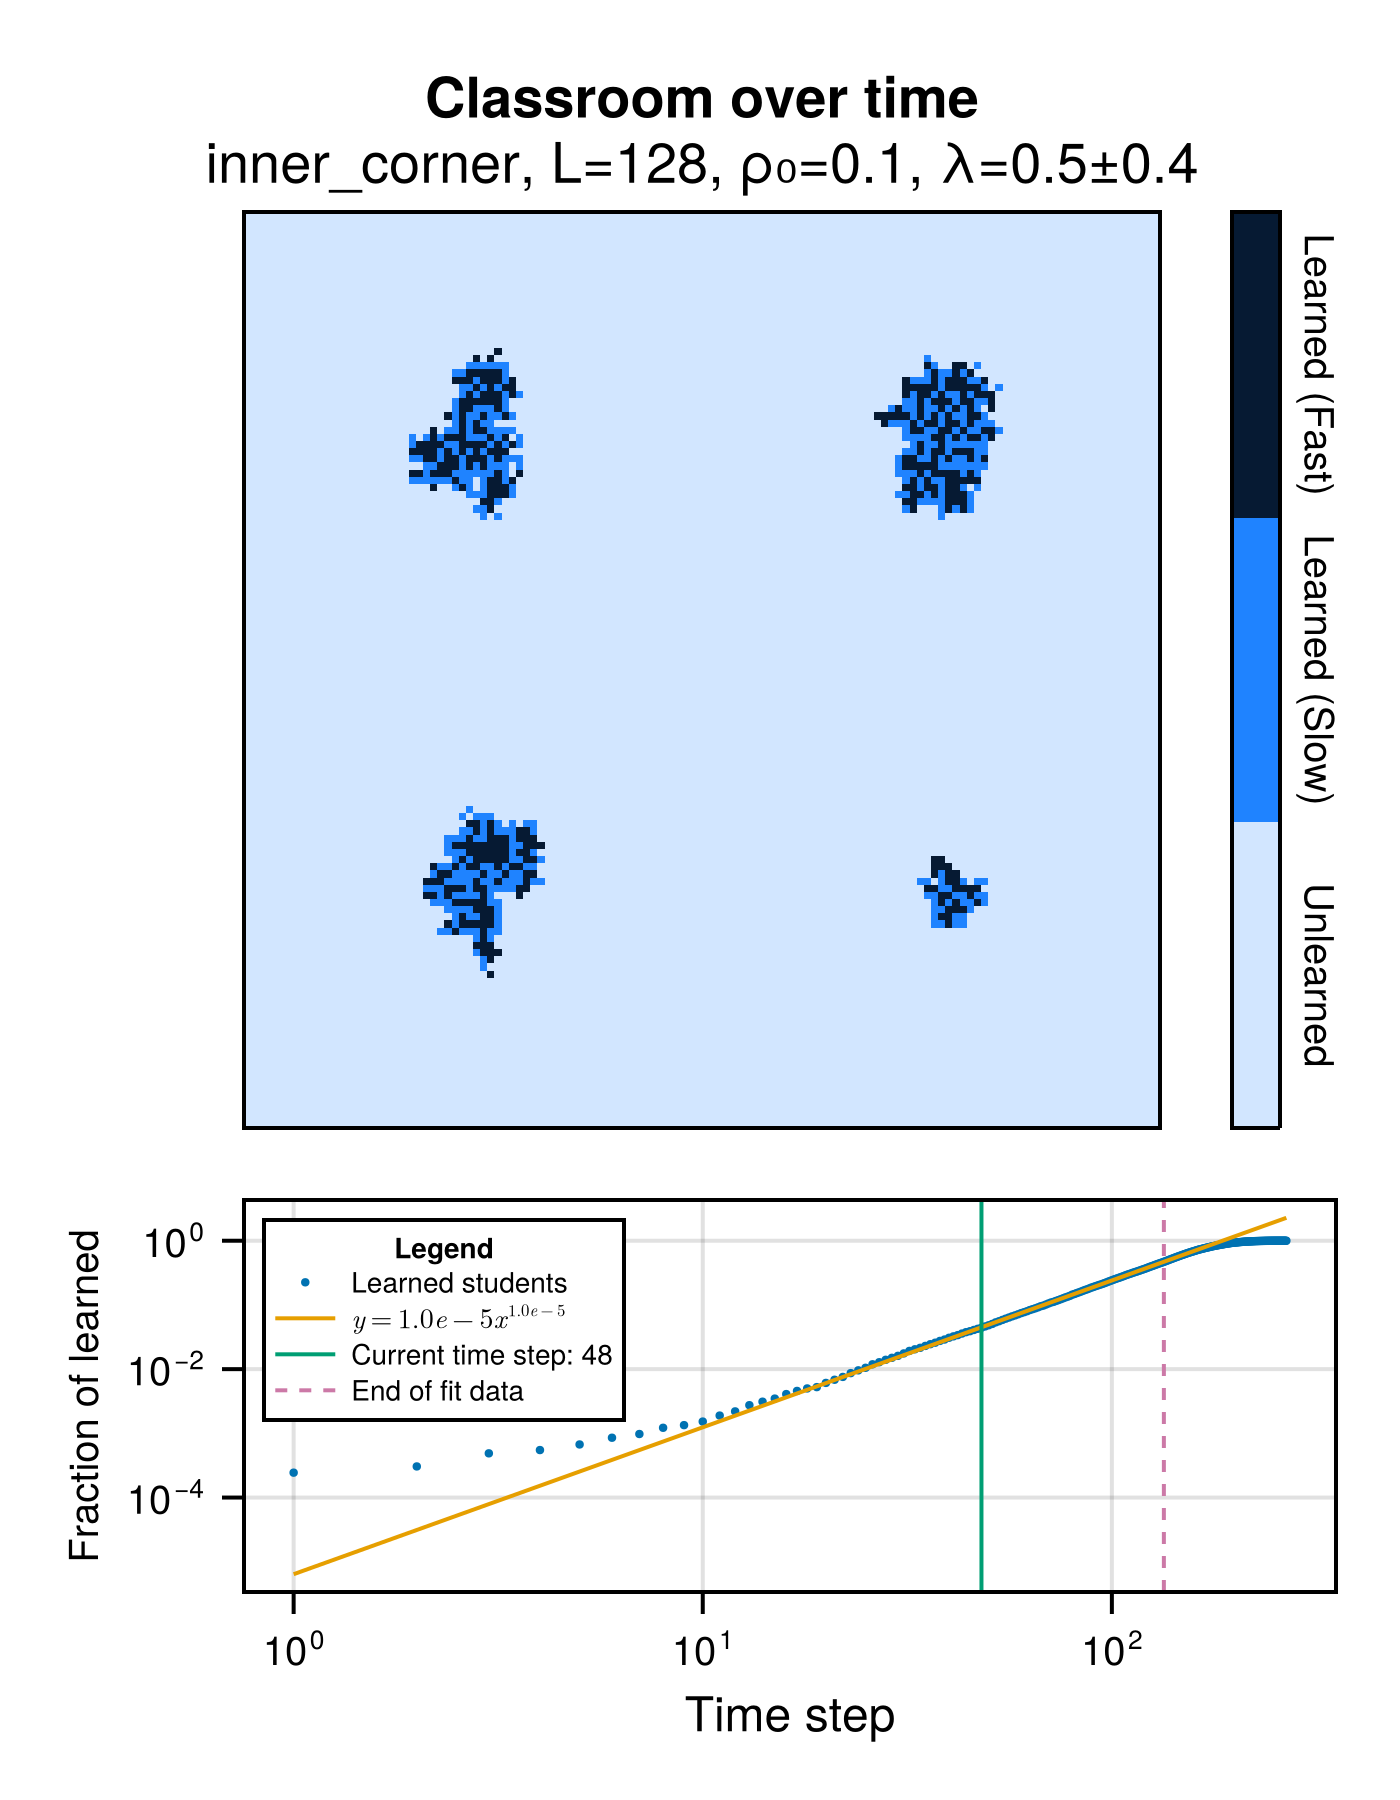
\includegraphics[width=0.40\textwidth]{figures/2D-BPCAIH-analysis/class evolutions/low rho/2DBPCAIH-inner_corner-128-0.1-0.5-0.4-trial_3-48.png}}
   \subfigure[$t=69$]{\label{fig:2DBPCAIH class evolution low rho 69}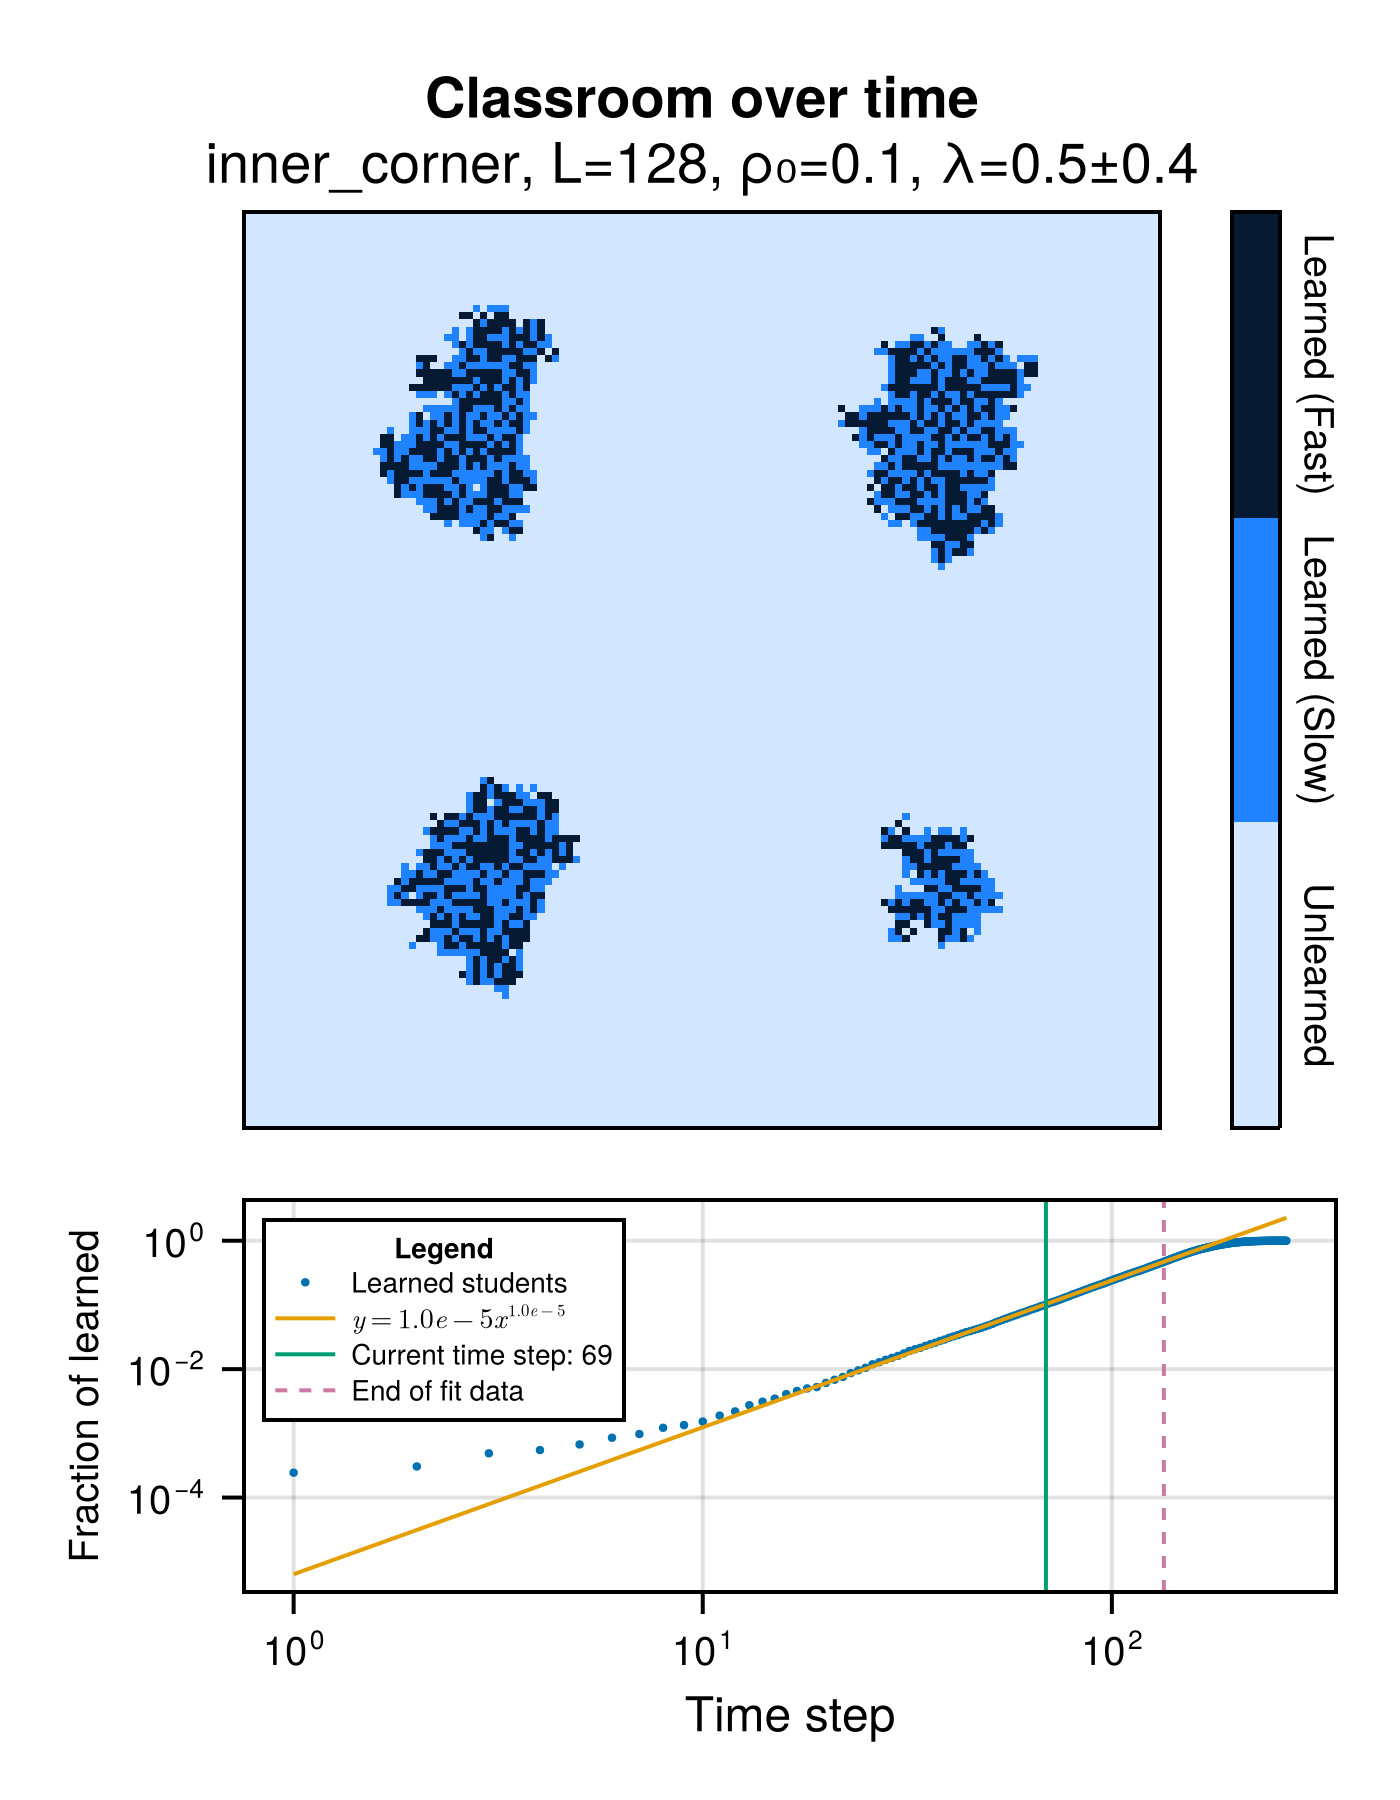
\includegraphics[width=0.40\textwidth]{figures/2D-BPCAIH-analysis/class evolutions/low rho/2DBPCAIH-inner_corner-128-0.1-0.5-0.4-trial_3-69.png}}
   \subfigure[$t=128$]{\label{fig:2DBPCAIH class evolution low rho 128}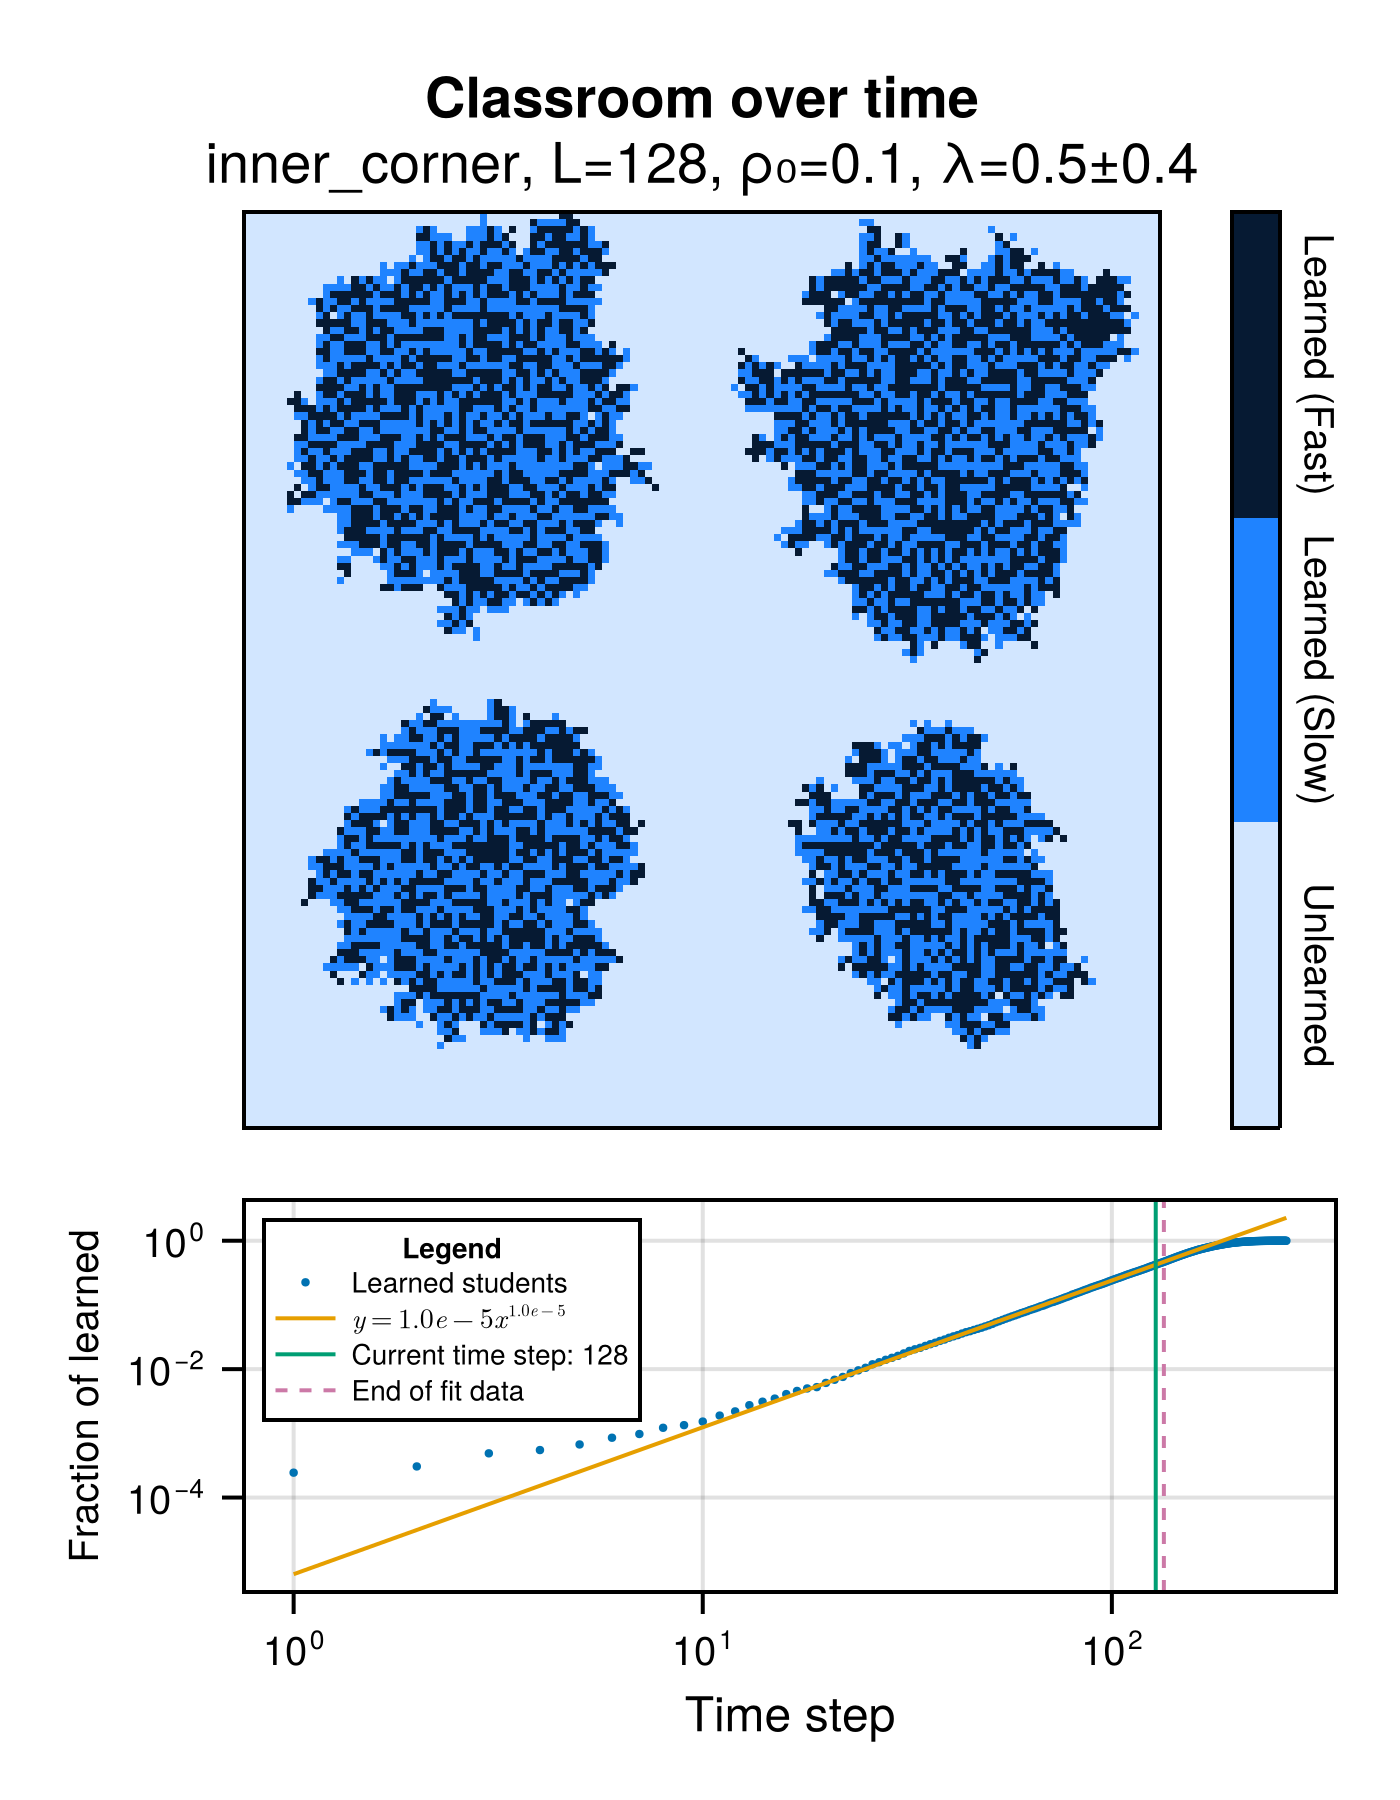
\includegraphics[width=0.40\textwidth]{figures/2D-BPCAIH-analysis/class evolutions/low rho/2DBPCAIH-inner_corner-128-0.1-0.5-0.4-trial_3-128.png}}
   \subfigure[$t=200$]{\label{fig:2DBPCAIH class evolution low rho 200}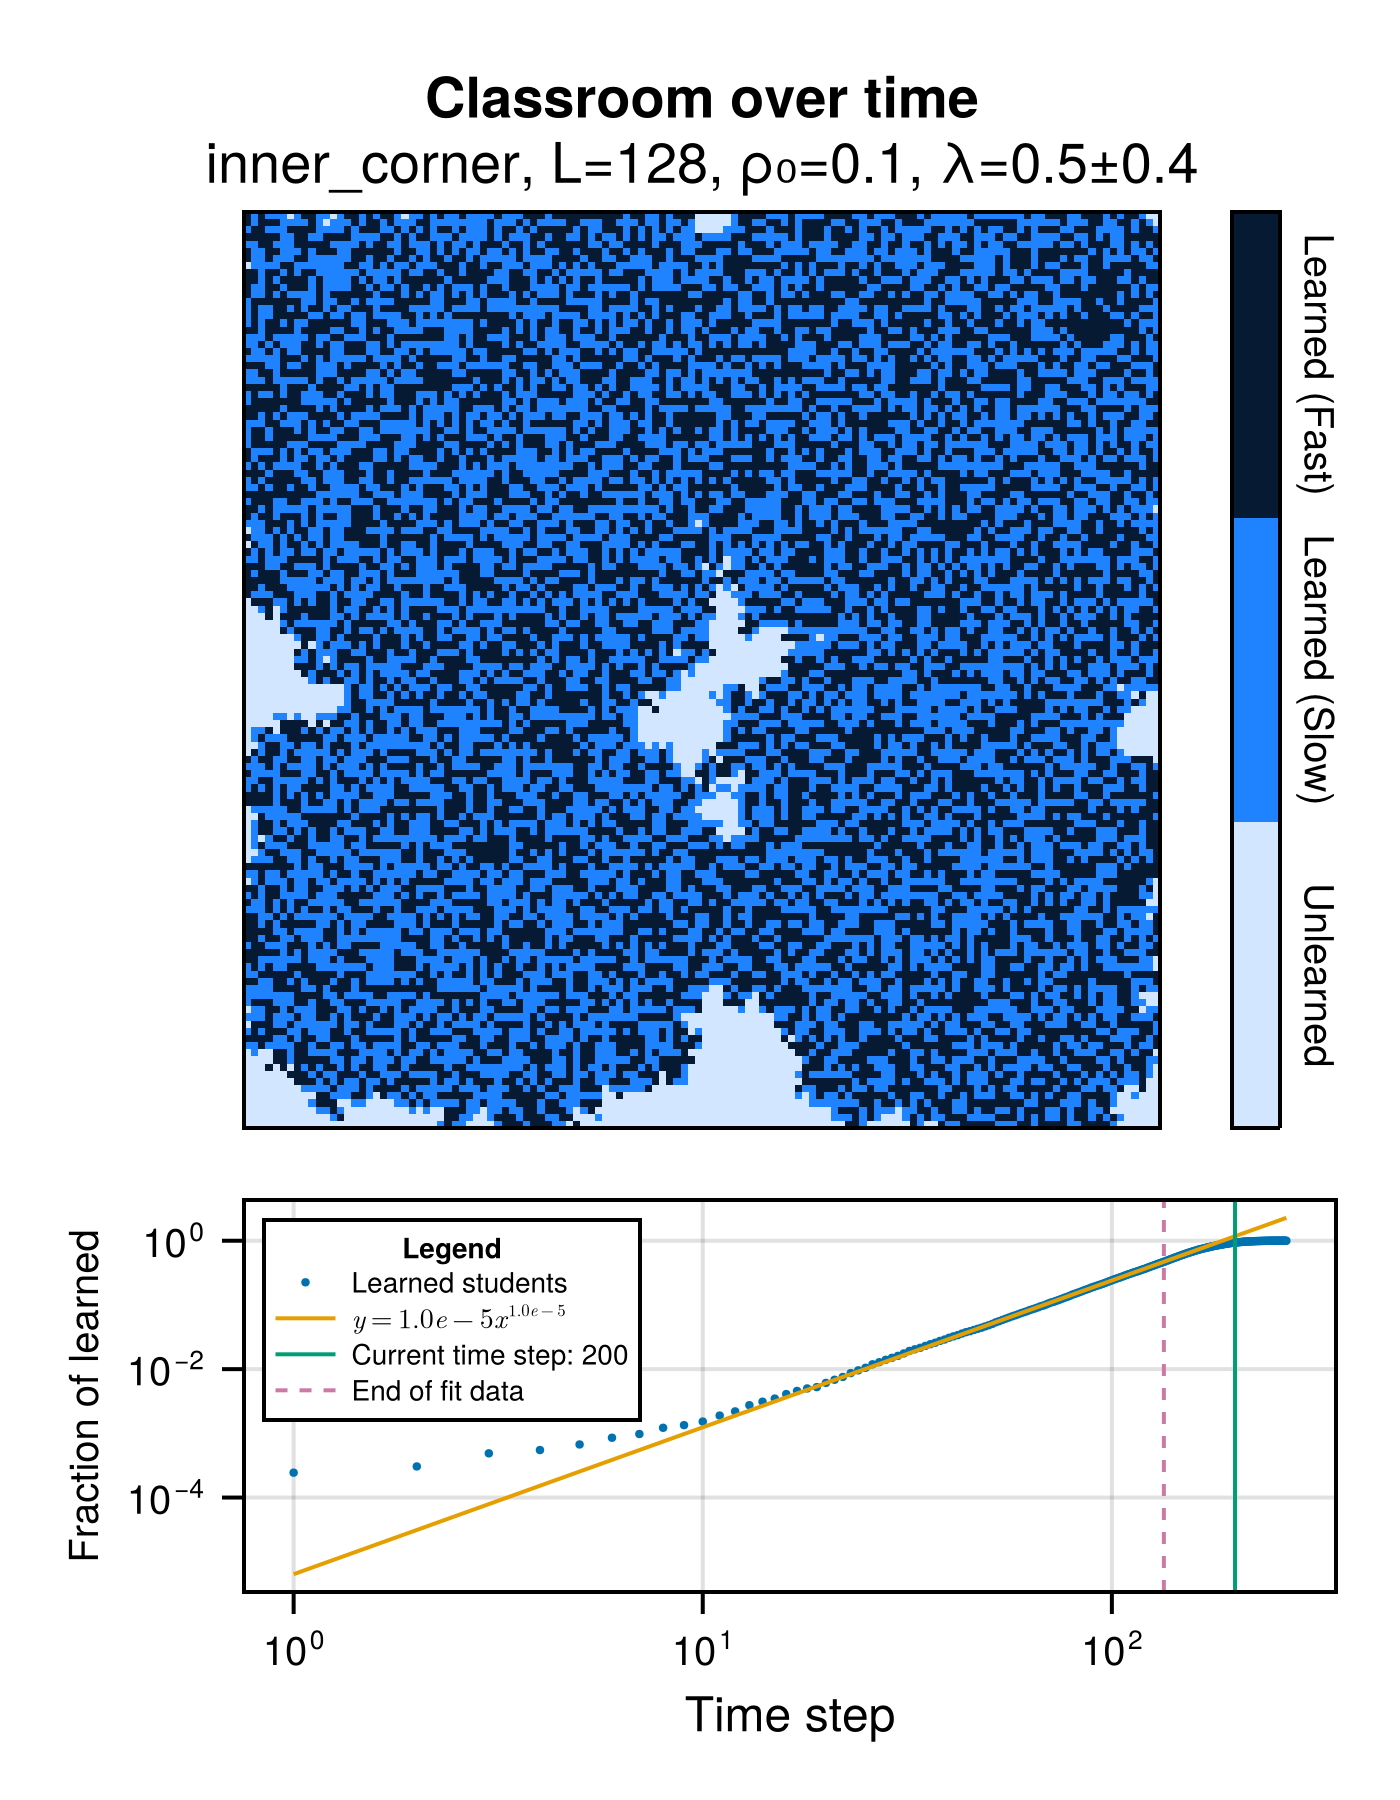
\includegraphics[width=0.40\textwidth]{figures/2D-BPCAIH-analysis/class evolutions/low rho/2DBPCAIH-inner_corner-128-0.1-0.5-0.4-trial_3-200.png}}
   \caption[Example classroom evolution for heterogeneous PI set up with low positional learning factor $\rho_0$ and high heterogeneity $\delta\lambda$]{Sample classroom evolutions for PI with the inner corner SA with $L=128$ at different times $t$ for positional learning coefficient $\rho_0=0.1$, $\delta\lambda = 0.4$.
   Dark blue squares represent learned students with learning rate $\lambda = \lambda_0 + \delta\lambda$, blue squares represent learned students with learning rate $\lambda = \lambda_0 - \delta\lambda$, and light blue squares represent unlearned students.
   The accompanying graph shows the fraction of learned students as a function time step.
   The blue dots represent data points. 
   The yellow line shows the power law fit.
   The pink dashed vertical line shows where we truncate the data for fitting the power law.
   The green vertical line shows the current time step in the simulation.
   }
   \label{fig:2DBPCAIH sample class evolution low rho}
\end{figure}

\begin{figure}[htbp!]
   \centering
   \subfigure[$t=5$]{\label{fig:2DBPCAIH class evolution high rho 5}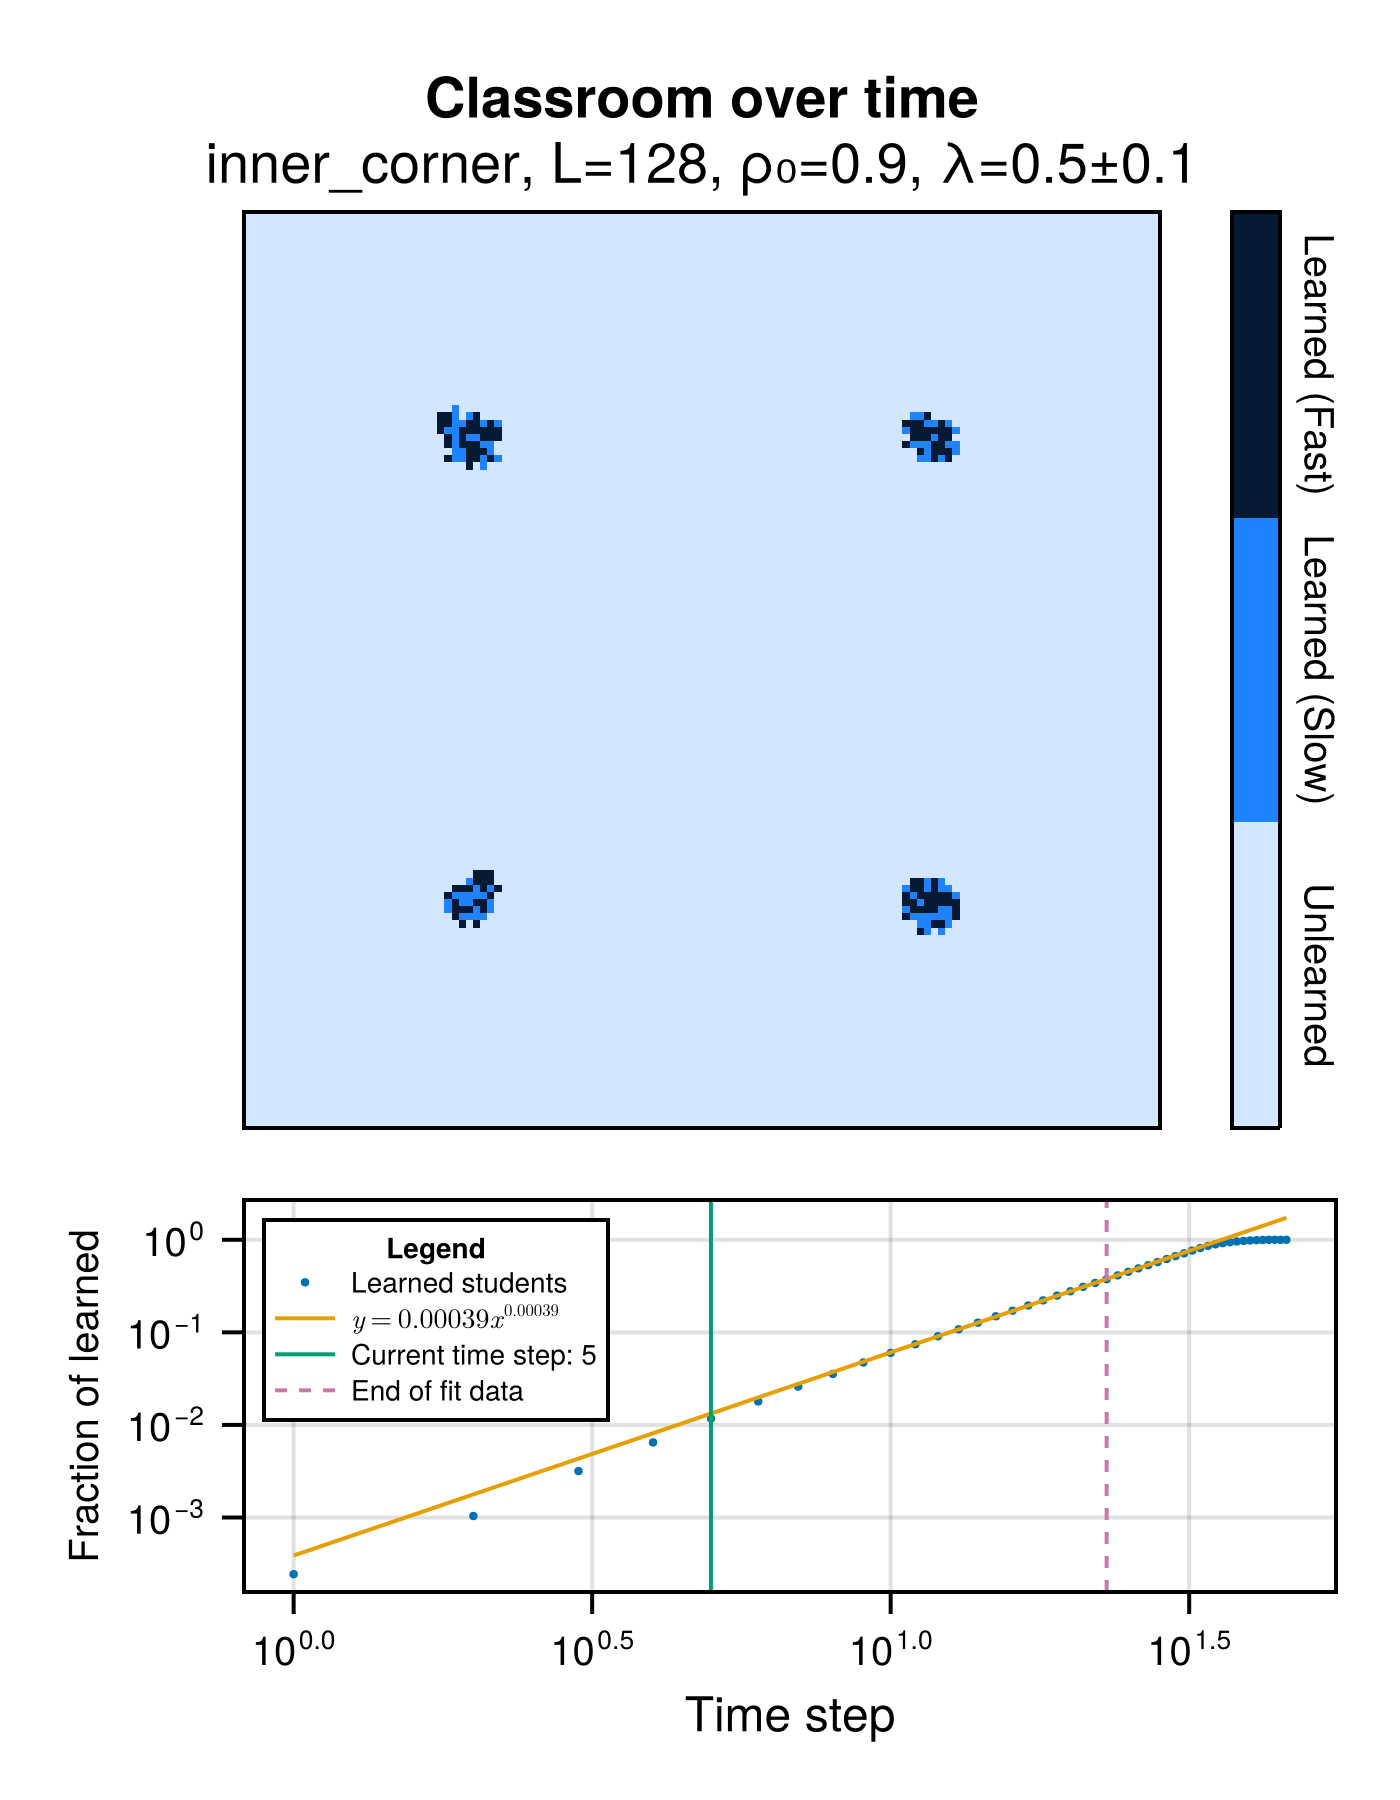
\includegraphics[width=0.40\textwidth]{figures/2D-BPCAIH-analysis/class evolutions/high rho/2DBPCAIH-inner_corner-128-0.9-0.5-0.1-trial_3-5.png}}
   \subfigure[$t=16$]{\label{fig:2DBPCAIH class evolution high rho 16}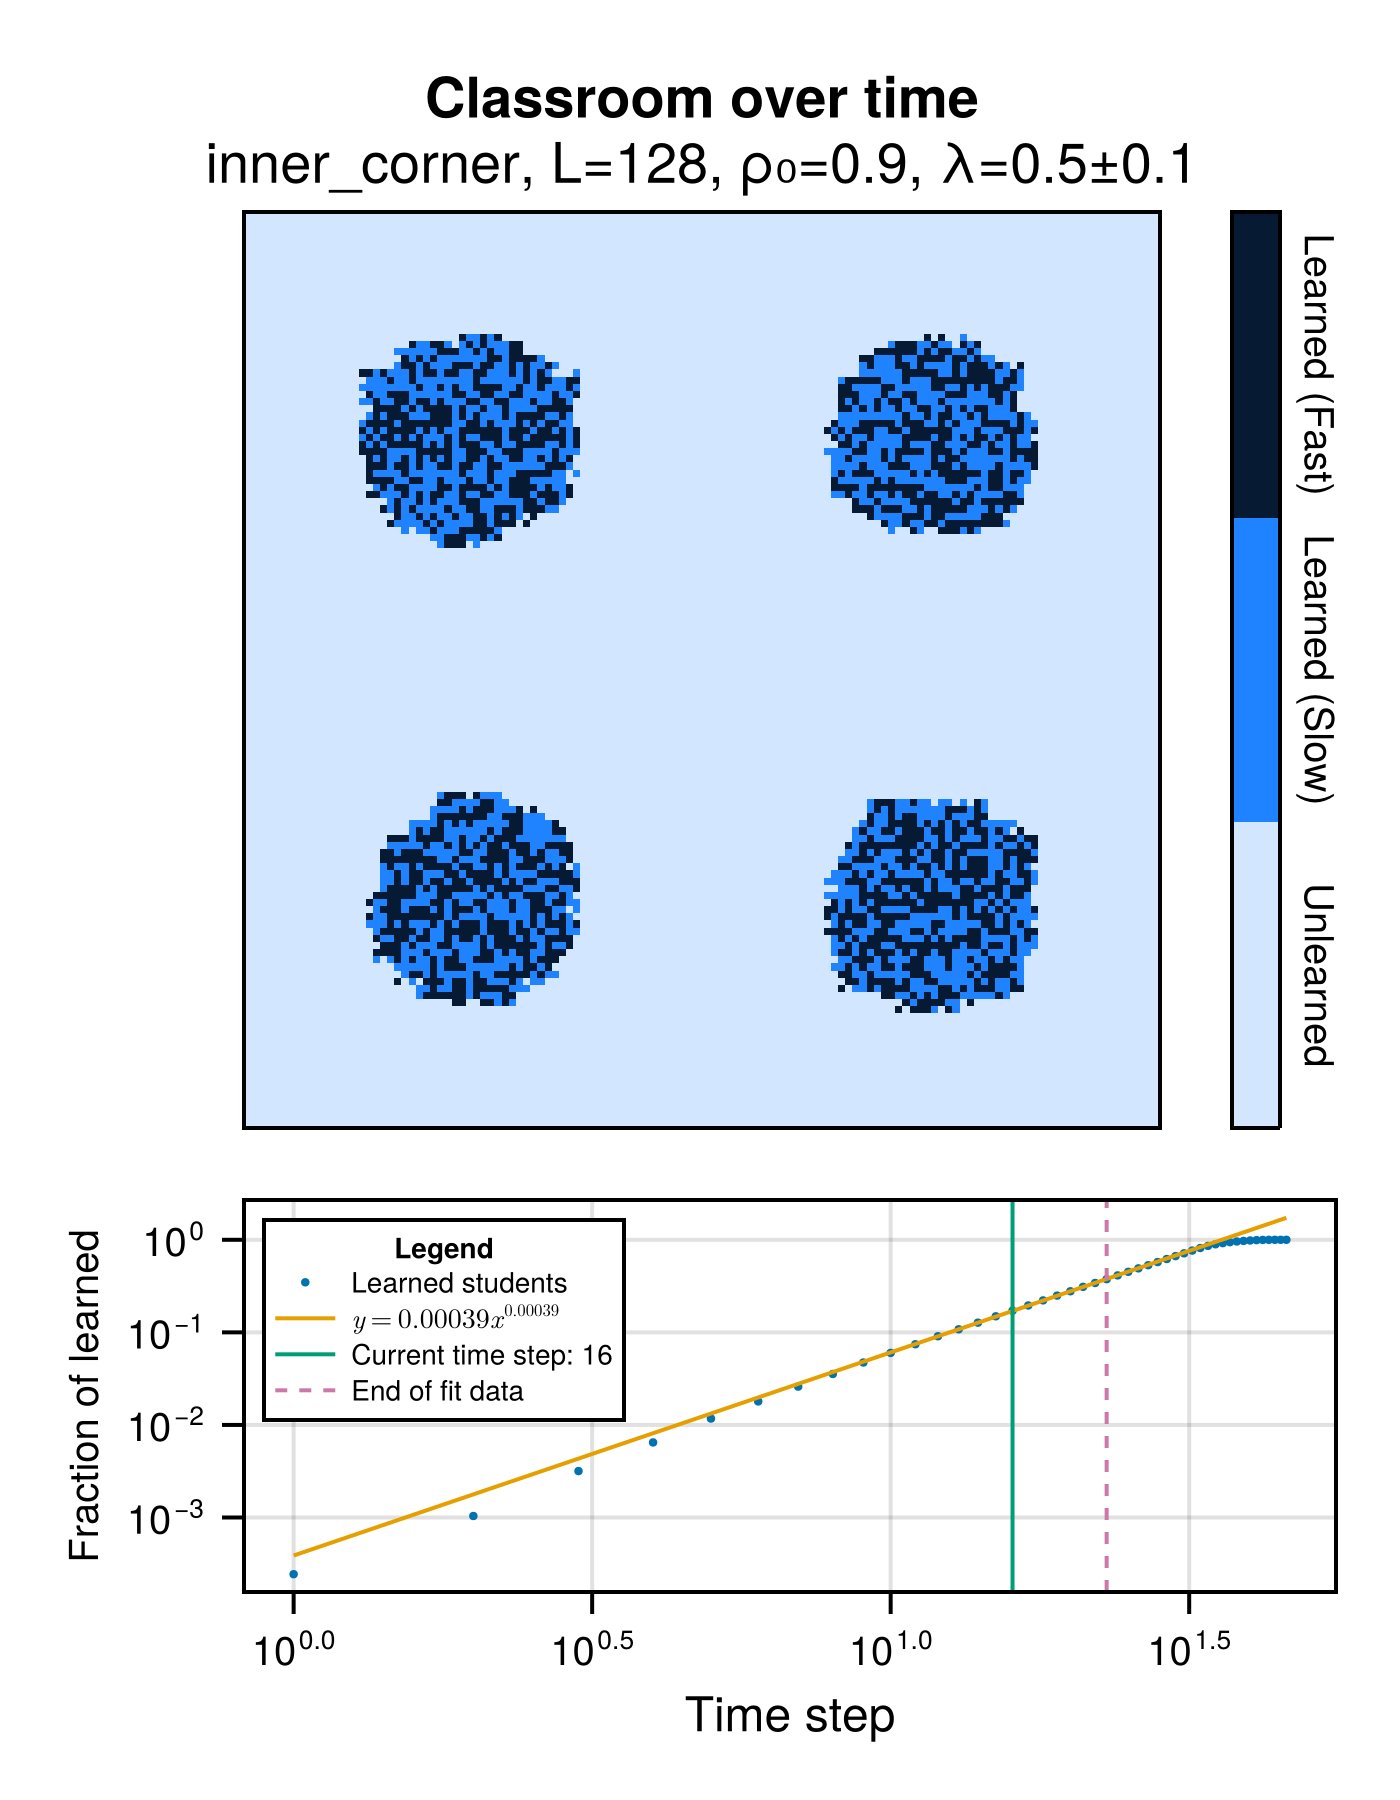
\includegraphics[width=0.40\textwidth]{figures/2D-BPCAIH-analysis/class evolutions/high rho/2DBPCAIH-inner_corner-128-0.9-0.5-0.1-trial_3-16.png}}
   \subfigure[$t=30$]{\label{fig:2DBPCAIH class evolution high rho 30}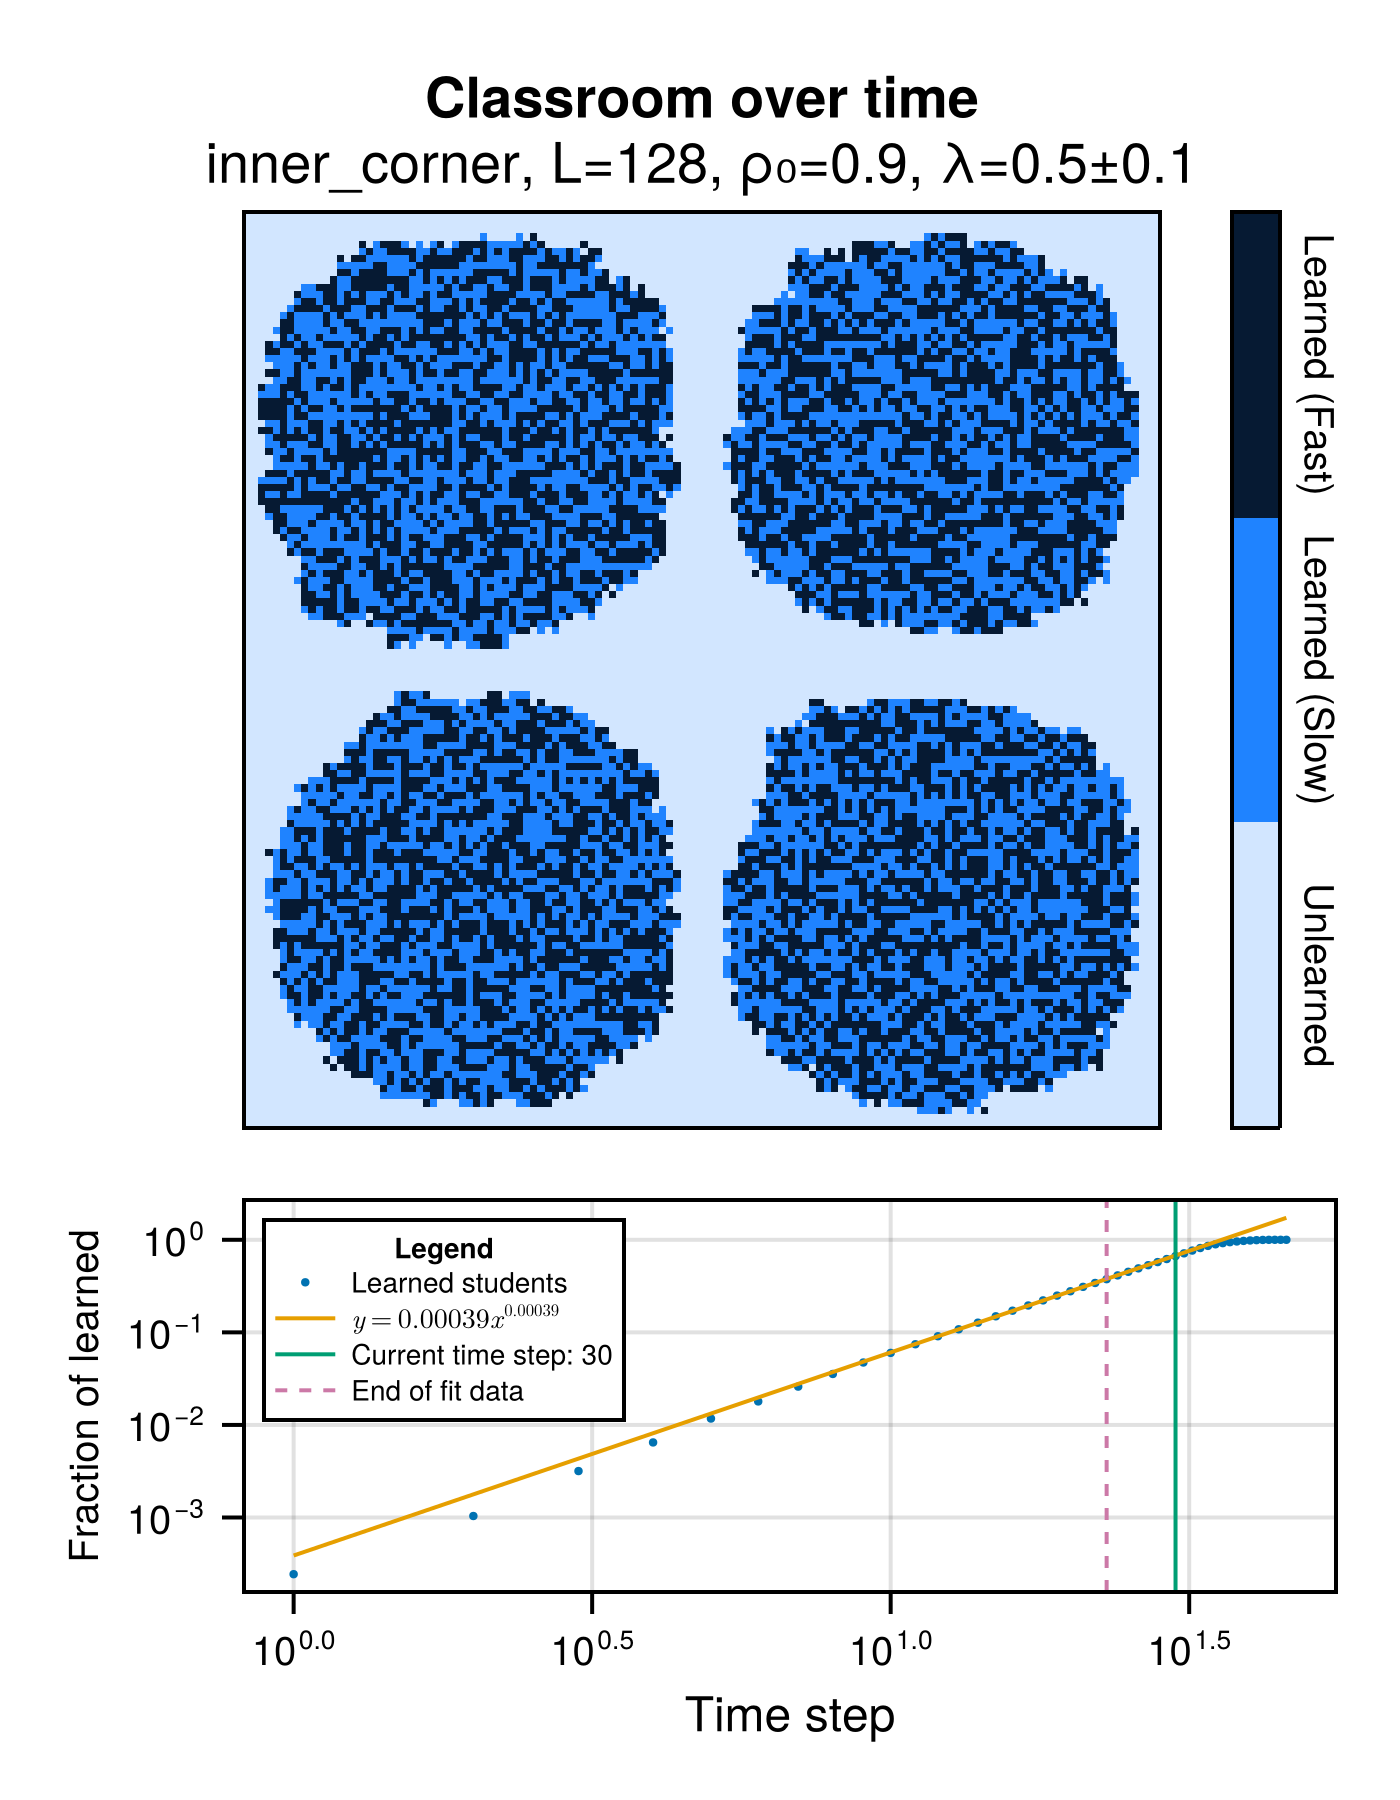
\includegraphics[width=0.40\textwidth]{figures/2D-BPCAIH-analysis/class evolutions/high rho/2DBPCAIH-inner_corner-128-0.9-0.5-0.1-trial_3-30.png}}
   \subfigure[$t=36$]{\label{fig:2DBPCAIH class evolution high rho 36}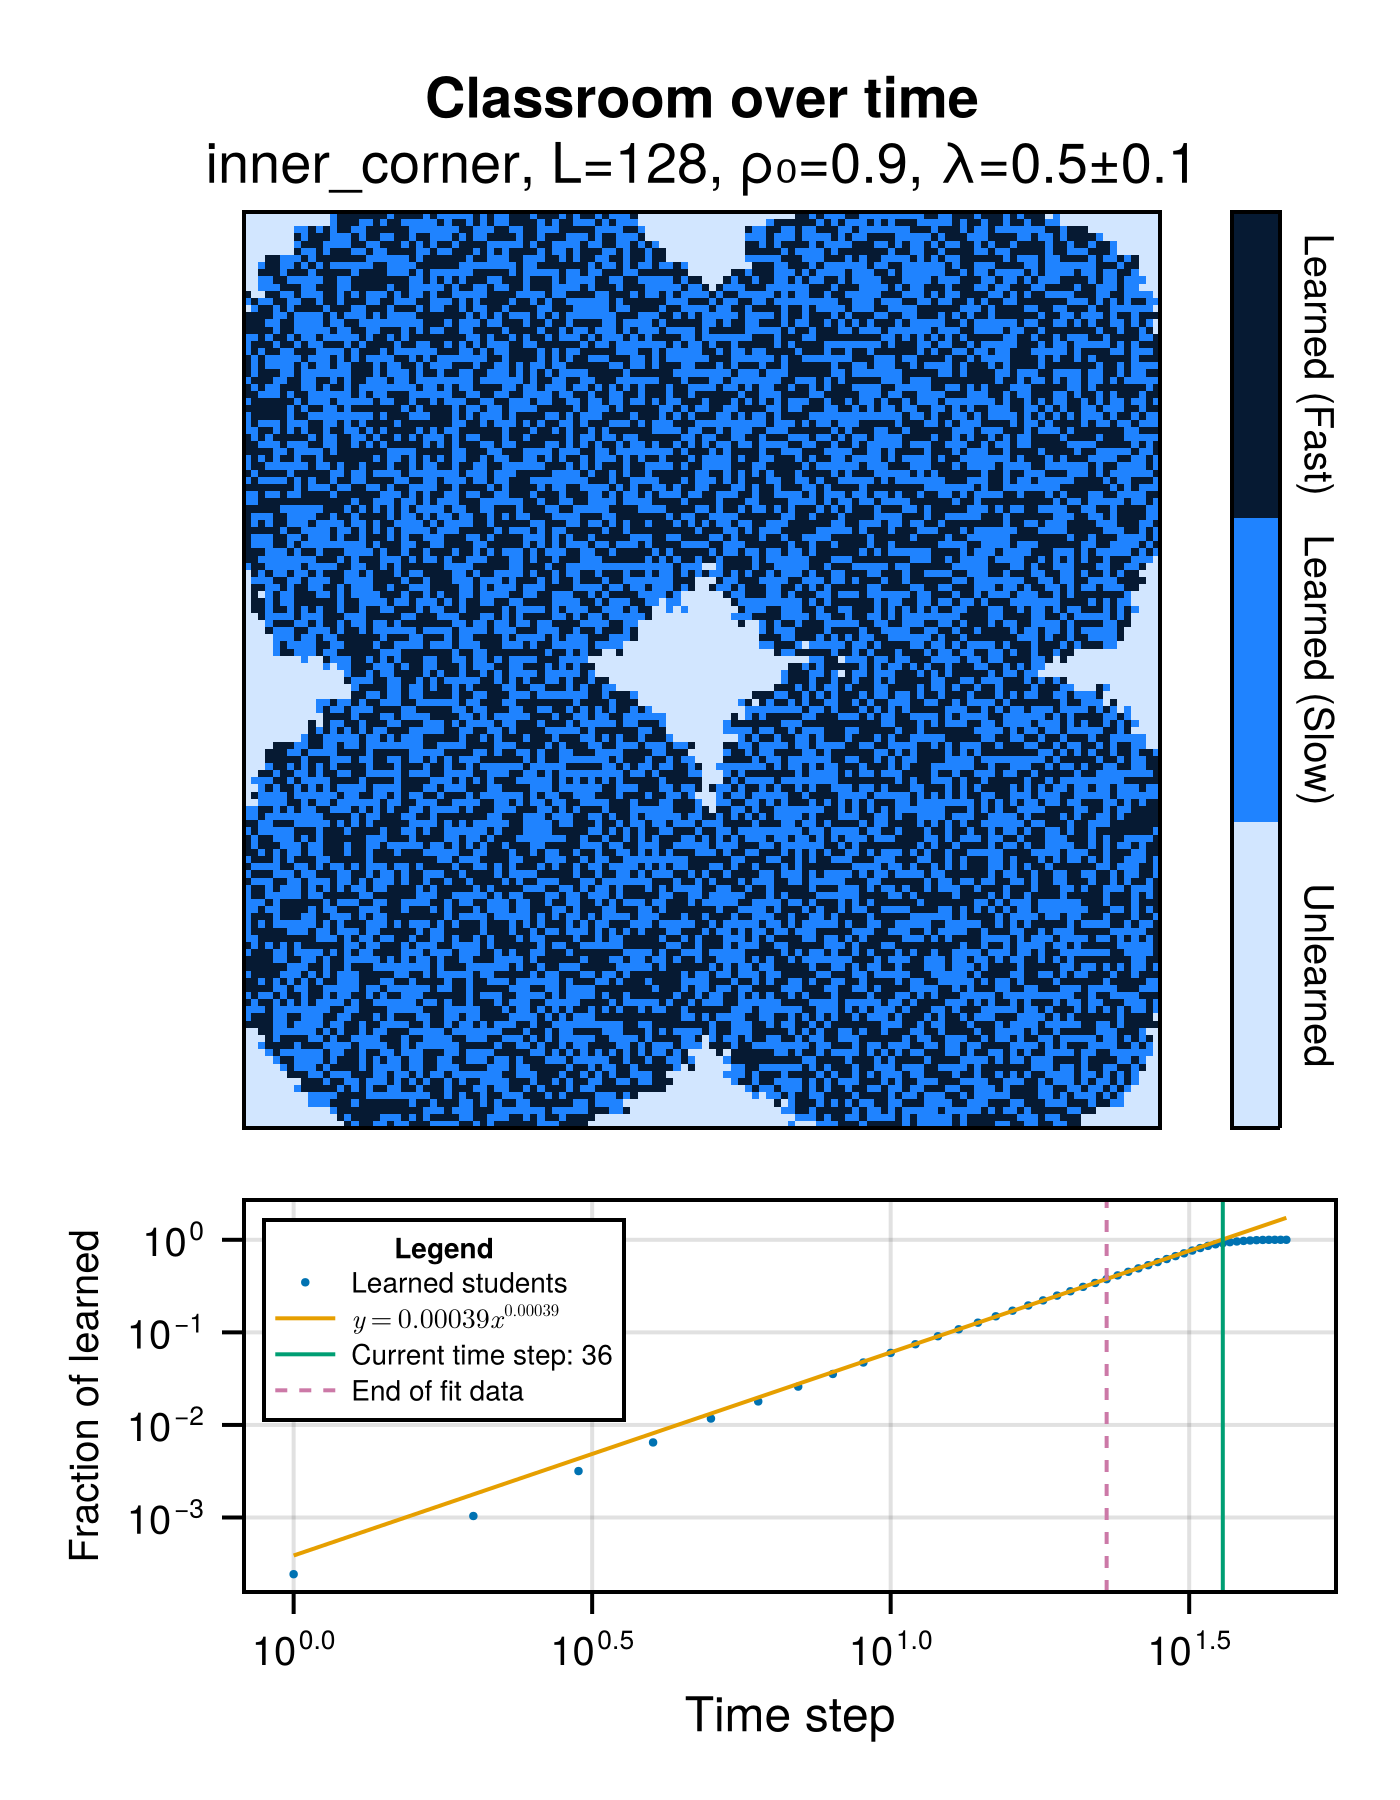
\includegraphics[width=0.40\textwidth]{figures/2D-BPCAIH-analysis/class evolutions/high rho/2DBPCAIH-inner_corner-128-0.9-0.5-0.1-trial_3-36.png}}   
   \caption[Example classroom evolution for heterogeneous PI set up with high positional learning factor $\rho_0$ and low heterogeneity $\delta\lambda$]{Sample classroom evolutions for PI with the inner corner SA with $L=128$ at different times $t$ for positional learning coefficient $\rho_0=0.9$, $\delta\lambda = 0.1$.
   Dark blue squares represent learned students with learning rate $\lambda = \lambda_0 + \delta\lambda$, blue squares represent learned students with learning rate $\lambda = \lambda_0 - \delta\lambda$, and light blue squares represent unlearned students.
   The accompanying graph shows the fraction of learned students as a function time step.
   The blue dots represent data points. 
   The yellow line shows the power law fit.
   The pink dashed vertical line shows where we truncate the data for fitting the power law.
   The green vertical line shows the current time step in the simulation.
   }
   \label{fig:2DBPCAIH sample class evolution high rho}
\end{figure}

\begin{figure}[htbp!]
   \centering
   \subfigure[$t=5$]{\label{fig:2DBPCAIH class evolution high rho high delta 5}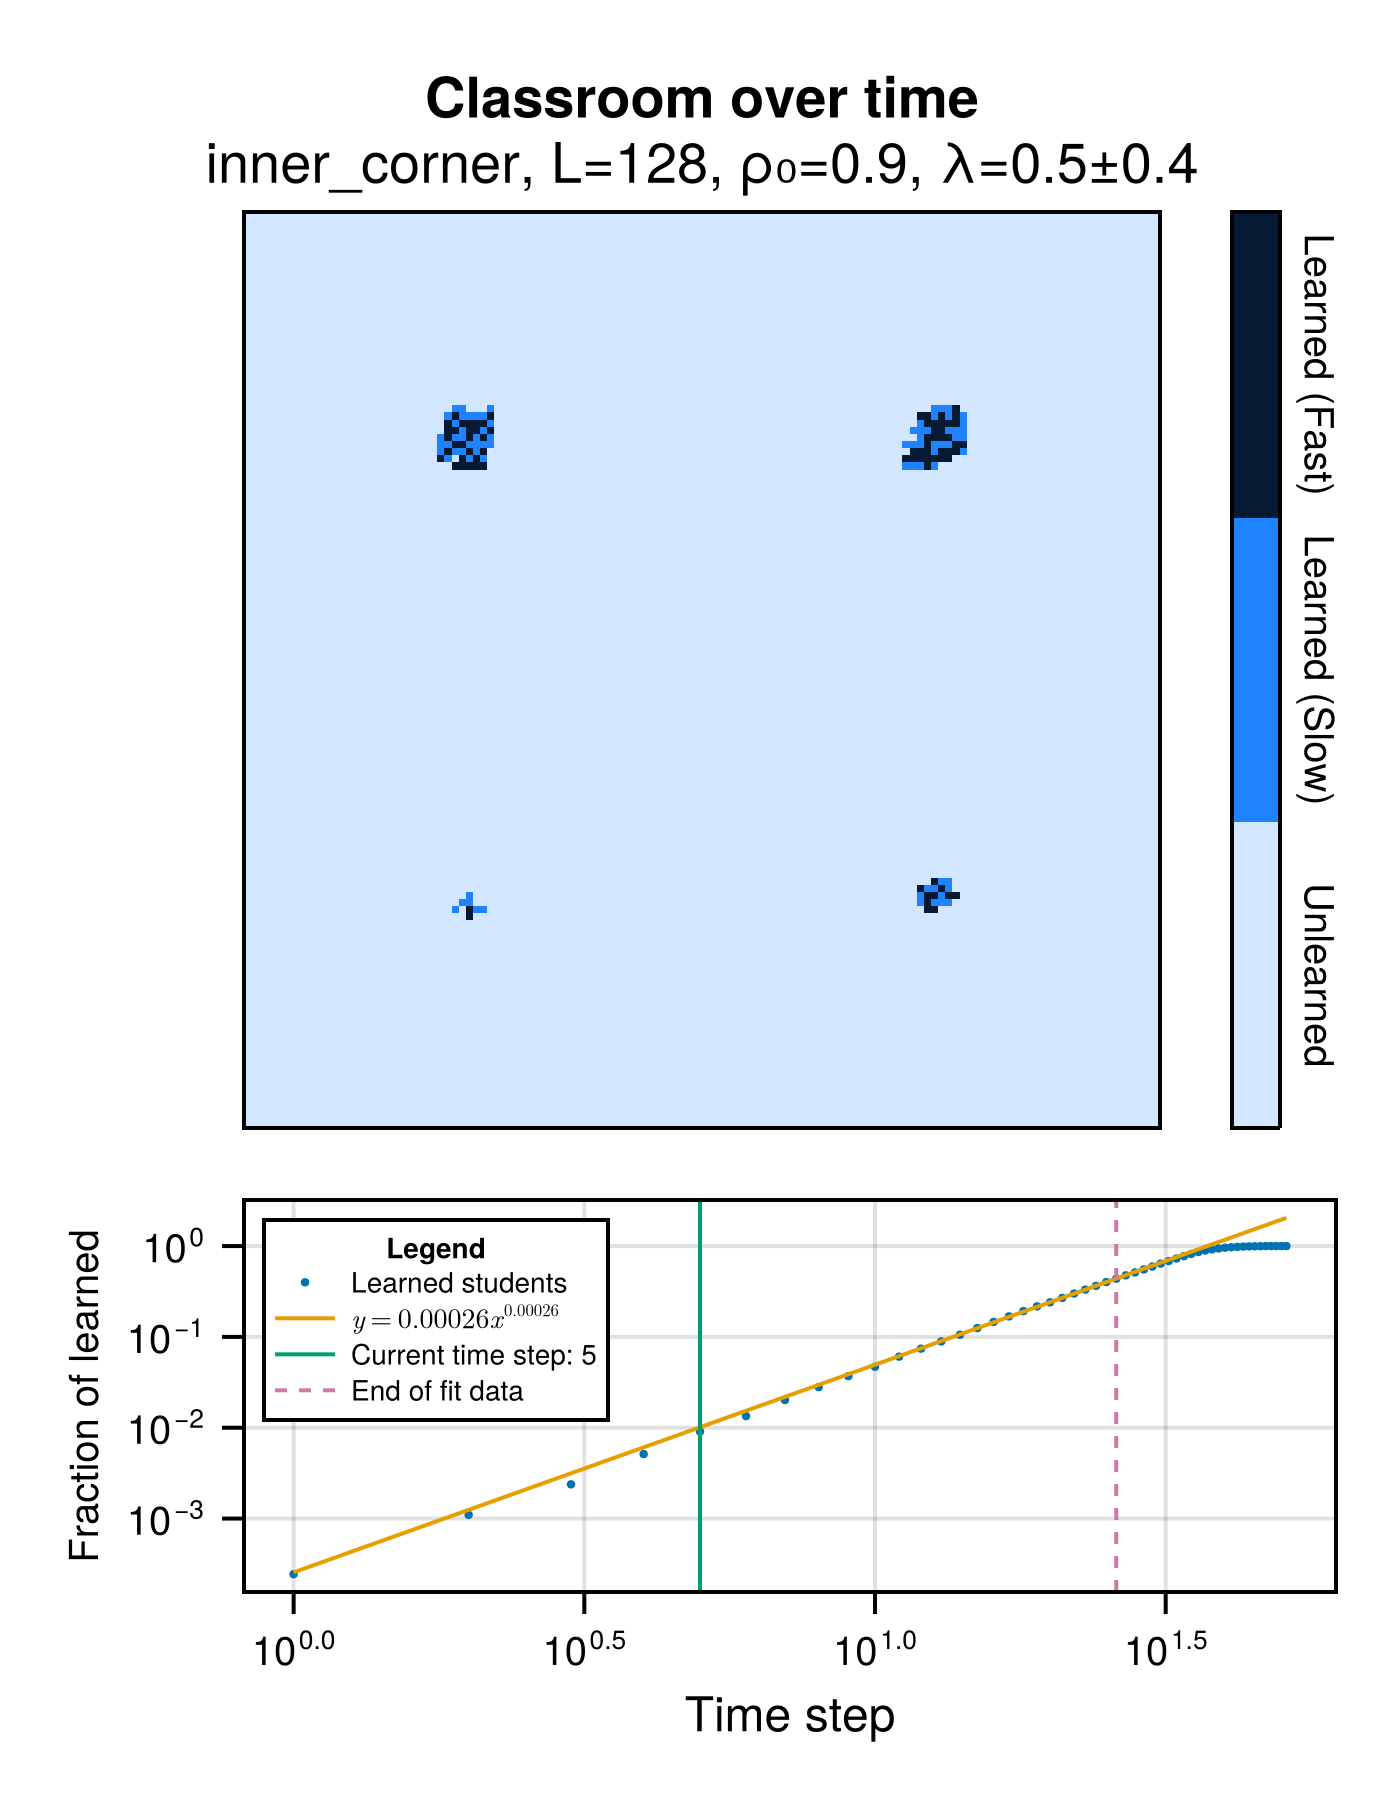
\includegraphics[width=0.40\textwidth]{figures/2D-BPCAIH-analysis/class evolutions/high rho high delta/2DBPCAIH-inner_corner-128-0.9-0.5-0.4-trial_3-5.png}}
   \subfigure[$t=13$]{\label{fig:2DBPCAIH class evolution high rho high delta 13}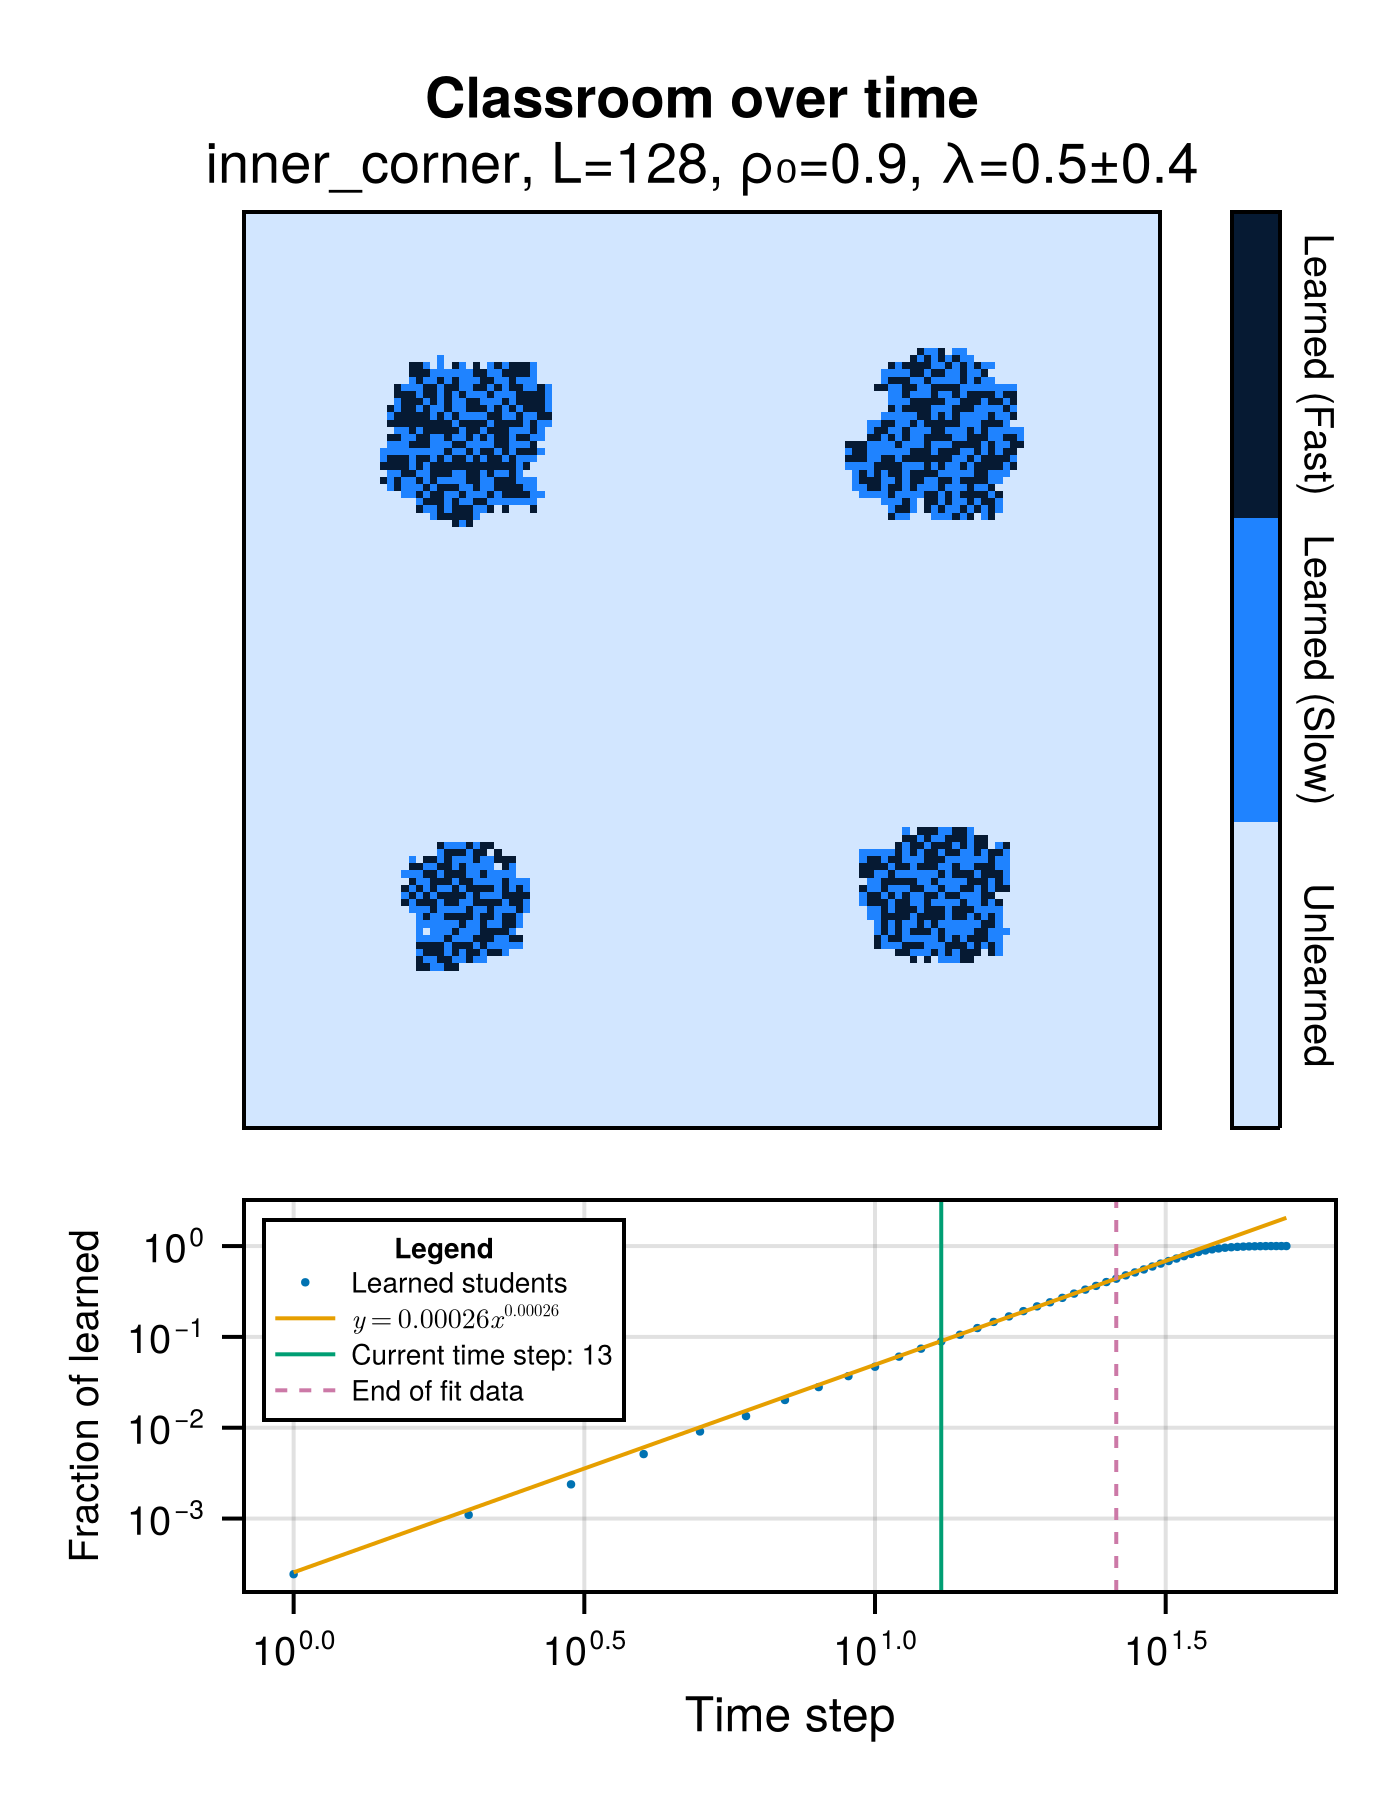
\includegraphics[width=0.40\textwidth]{figures/2D-BPCAIH-analysis/class evolutions/high rho high delta/2DBPCAIH-inner_corner-128-0.9-0.5-0.4-trial_3-13.png}}
   \subfigure[$t=19$]{\label{fig:2DBPCAIH class evolution high rho high delta 19}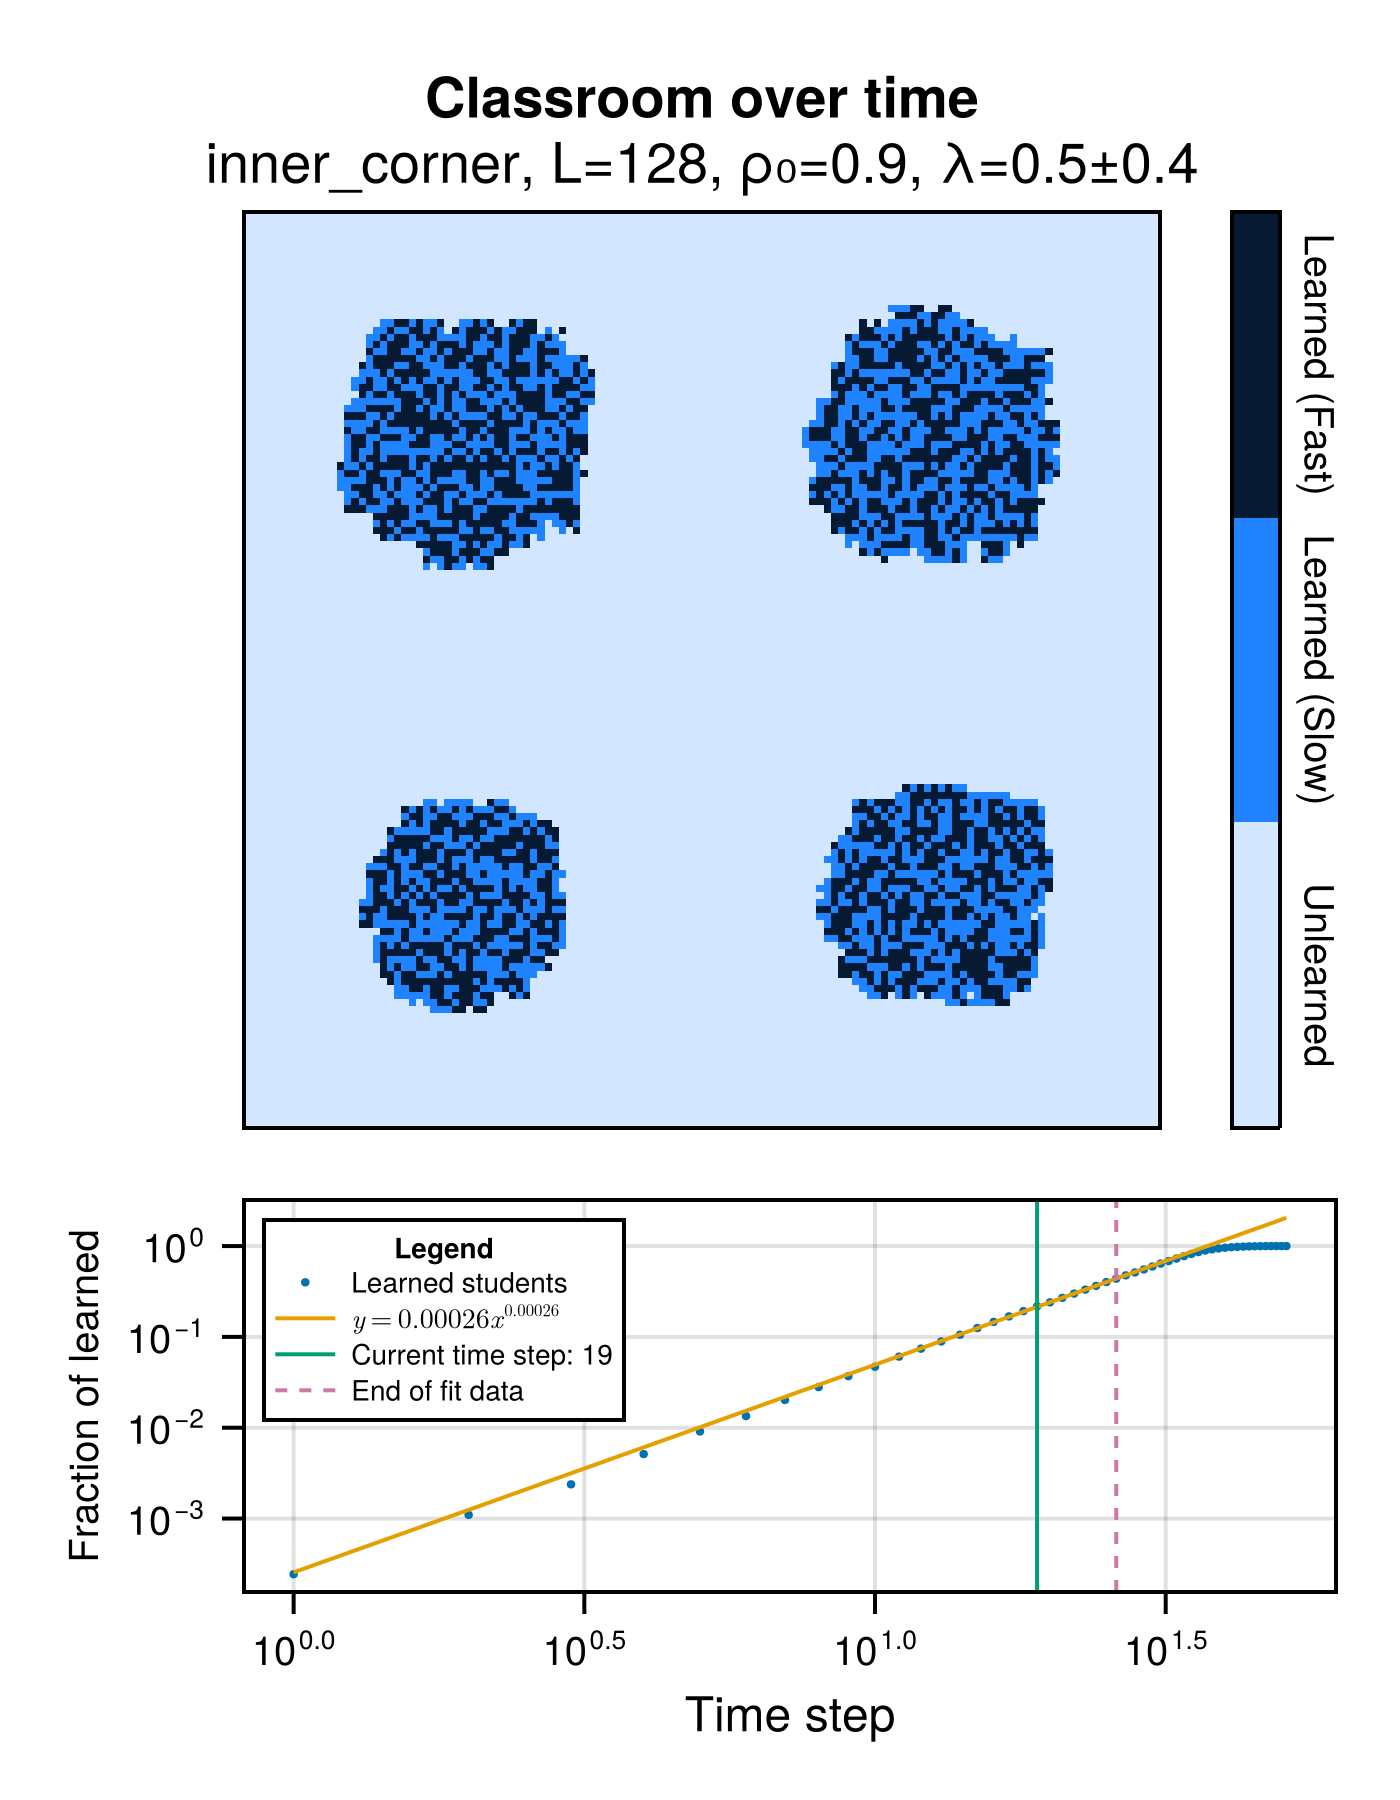
\includegraphics[width=0.40\textwidth]{figures/2D-BPCAIH-analysis/class evolutions/high rho high delta/2DBPCAIH-inner_corner-128-0.9-0.5-0.4-trial_3-19.png}}
   \subfigure[$t=29$]{\label{fig:2DBPCAIH class evolution high rho high delta 29}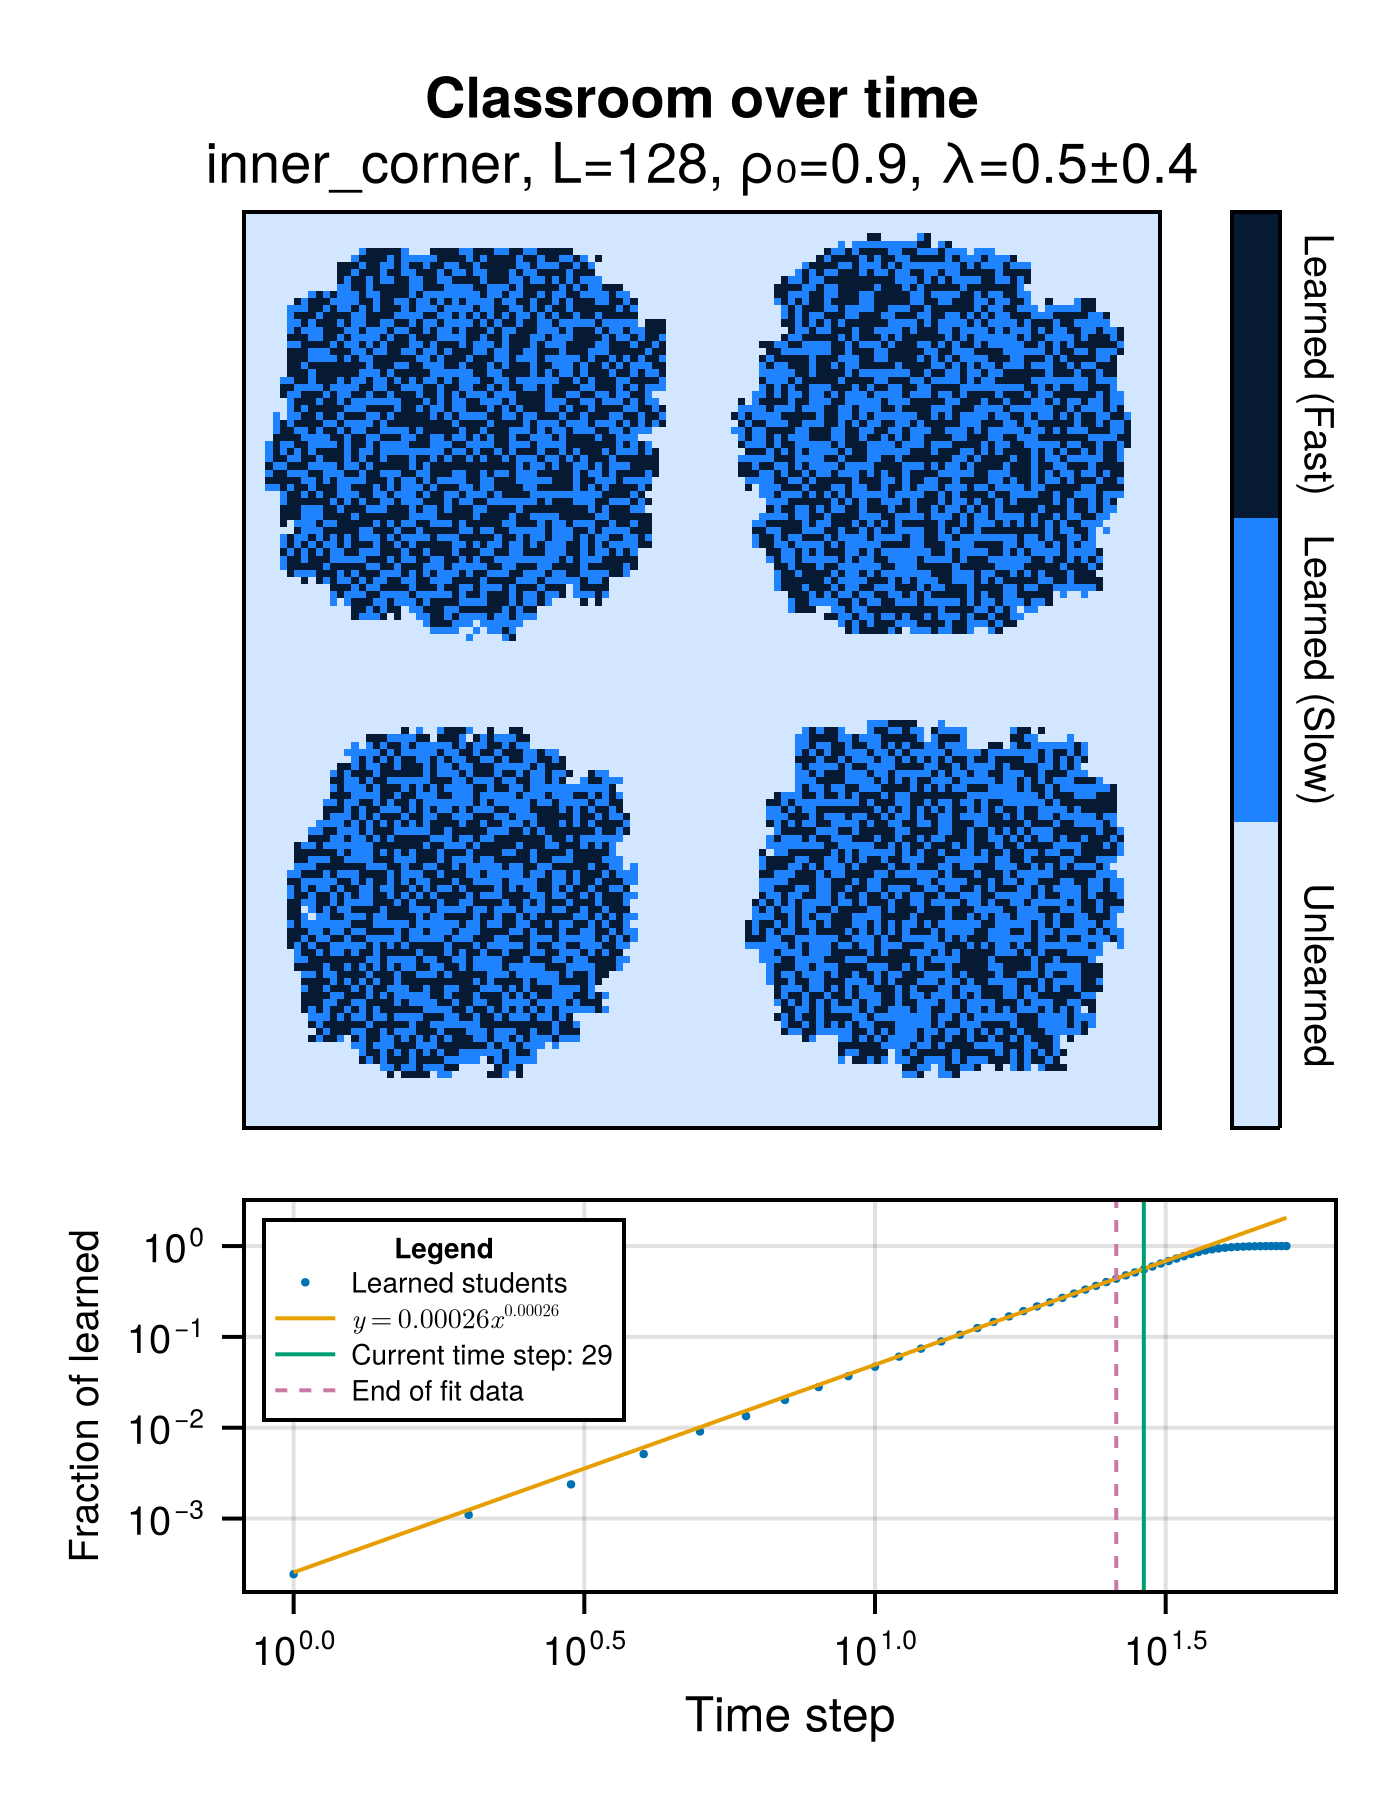
\includegraphics[width=0.40\textwidth]{figures/2D-BPCAIH-analysis/class evolutions/high rho high delta/2DBPCAIH-inner_corner-128-0.9-0.5-0.4-trial_3-29.png}}
   \caption[Example classroom evolution for heterogeneous PI set up with high positional learning factor $\rho_0$ and high heterogeneity $\delta\lambda$]{Sample classroom evolutions for PI with the inner corner SA with $L=128$ at different times $t$ for positional learning rate $\rho_0=0.9$, $\delta\lambda = 0.4$.
   Dark blue squares represent learned students with learning rate $\lambda = \lambda_0 + \delta\lambda$, blue squares represent learned students with learning rate $\lambda = \lambda_0 - \delta\lambda$, and light blue squares represent unlearned students.
   The accompanying graph shows the fraction of learned students as a function time step.
   The blue dots represent data points. 
   The yellow line shows the power law fit.
   The pink dashed vertical line shows where we truncate the data for fitting the power law.
   The green vertical line shows the current time step in the simulation.
   }
   \label{fig:2DBPCAIH sample class evolution high rho high delta}
\end{figure}

\subsection{Traditional Instruction}
For traditional instruction, even though the value of positional learning coefficient $\rho_0$ is still an important factor in determining class performance, the effect of $\delta\lambda$ is more pronounced compared to PI.
The trend we see in traditional instruction that is absent or less evident in PI, is that majority of the students that learn earlier in the simulations are fast learning students (Figure~\ref{fig:2DBPCAIH class evolution trad low rho high delta 2}). 
After this period, most of the simulation time is spent waiting for the slow learning students to learn.
This behavior is more pronounced for higher values of $\delta\lambda$ and lower values of $\rho_0$ as shown in Figure~\ref{fig:2DBPCAIH sample class evolution trad low rho high delta}.
This could explain the deviation from the power law fit at earlier times $t$ for the traditional model considering that the deviation shows that the class learning rate is higher than the fitted power law.

\begin{figure}[htbp!]
   \centering
   \subfigure[$t=2$]{\label{fig:2DBPCAIH class evolution trad low rho high delta 2}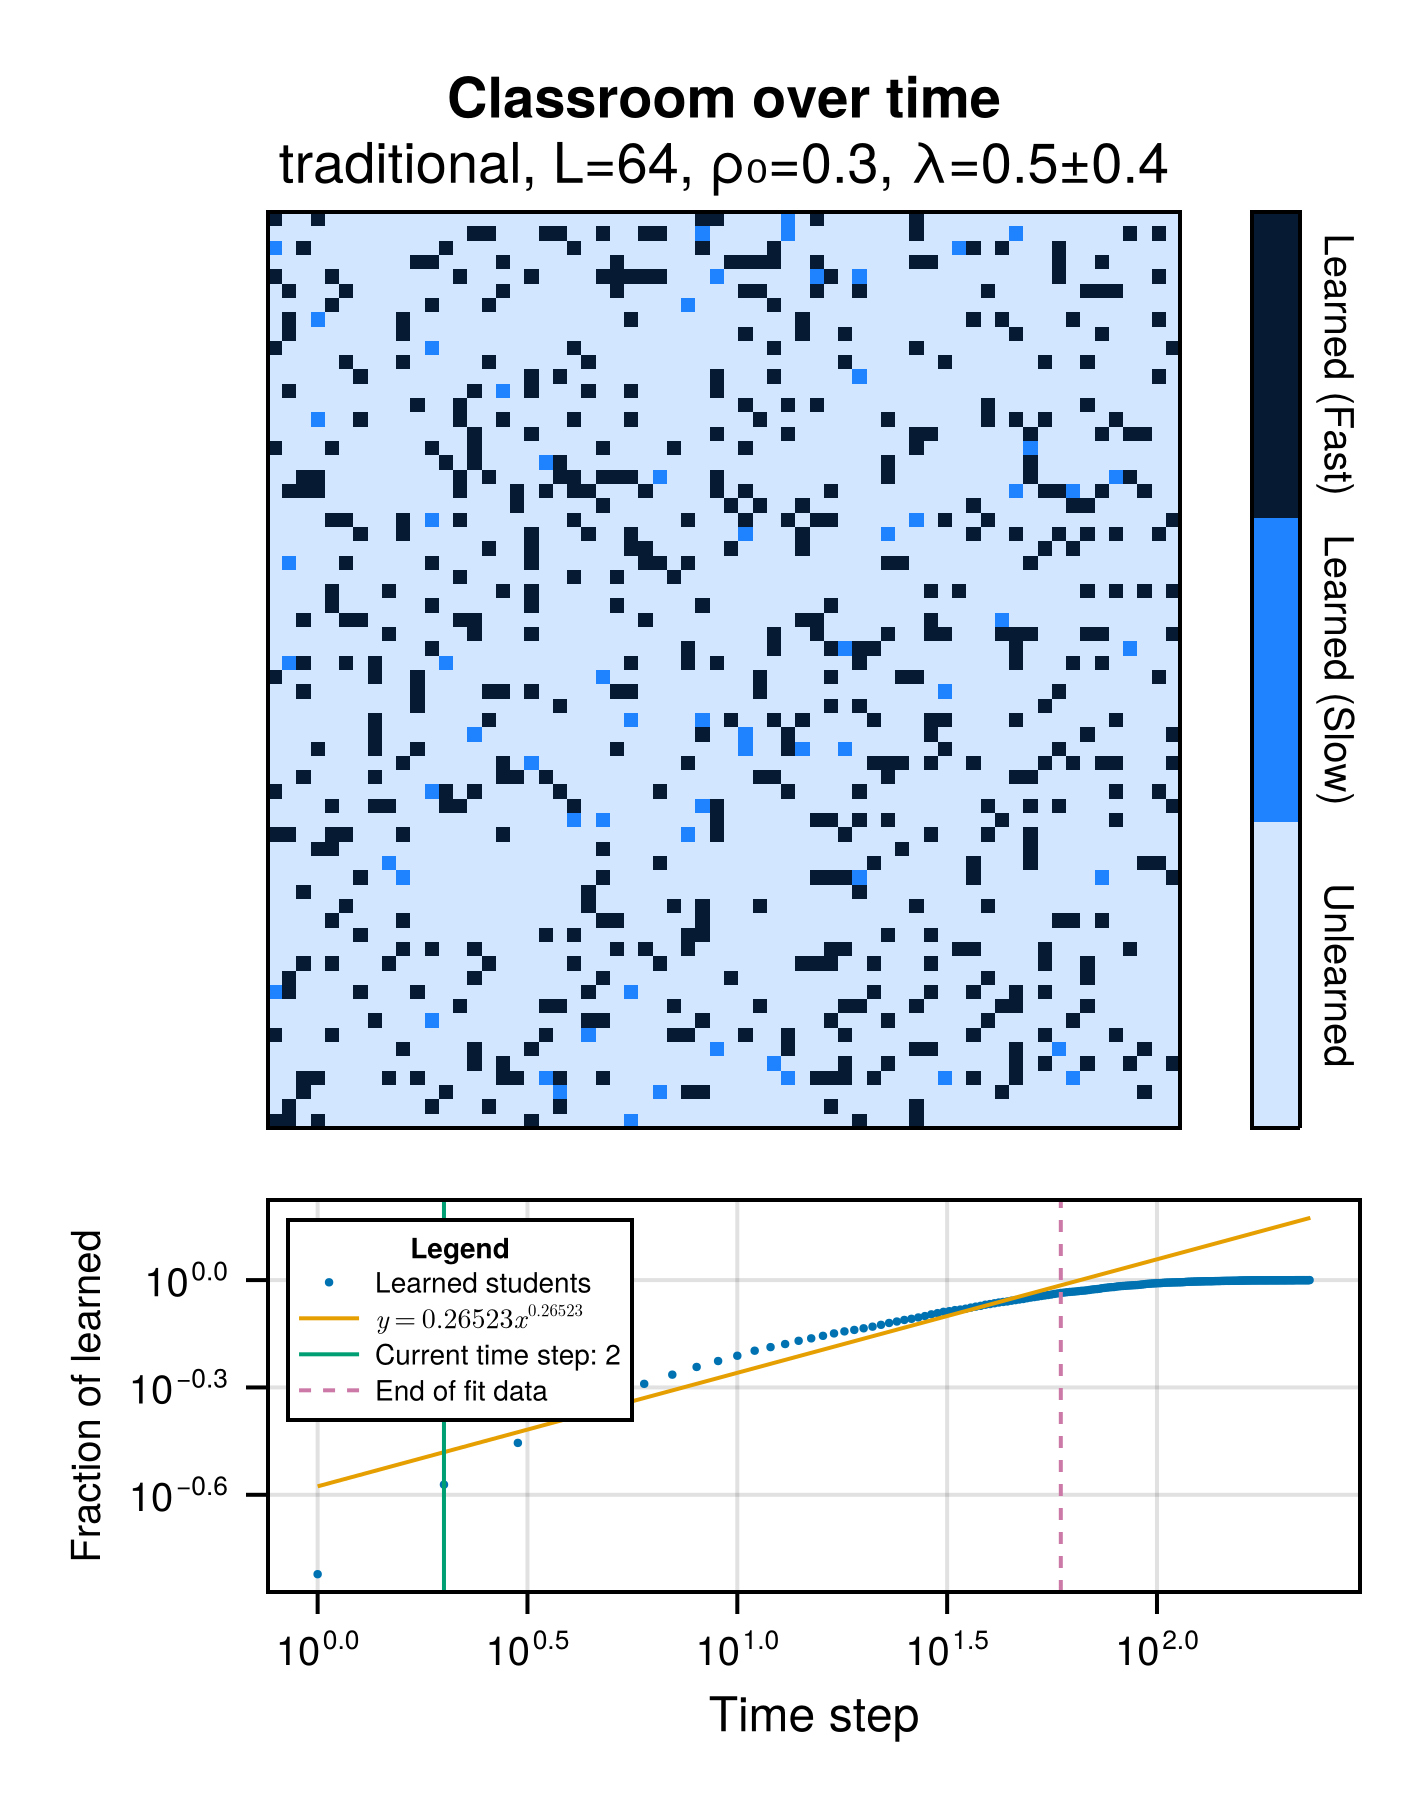
\includegraphics[width=0.40\textwidth]{figures/2D-BPCAIH-analysis/class evolutions/trad low rho high delta/2DBPCAIH-traditional-64-0.3-0.5-0.4-trial_3-2.png}}
   \subfigure[$t=13$]{\label{fig:2DBPCAIH class evolution trad low rho high delta 13}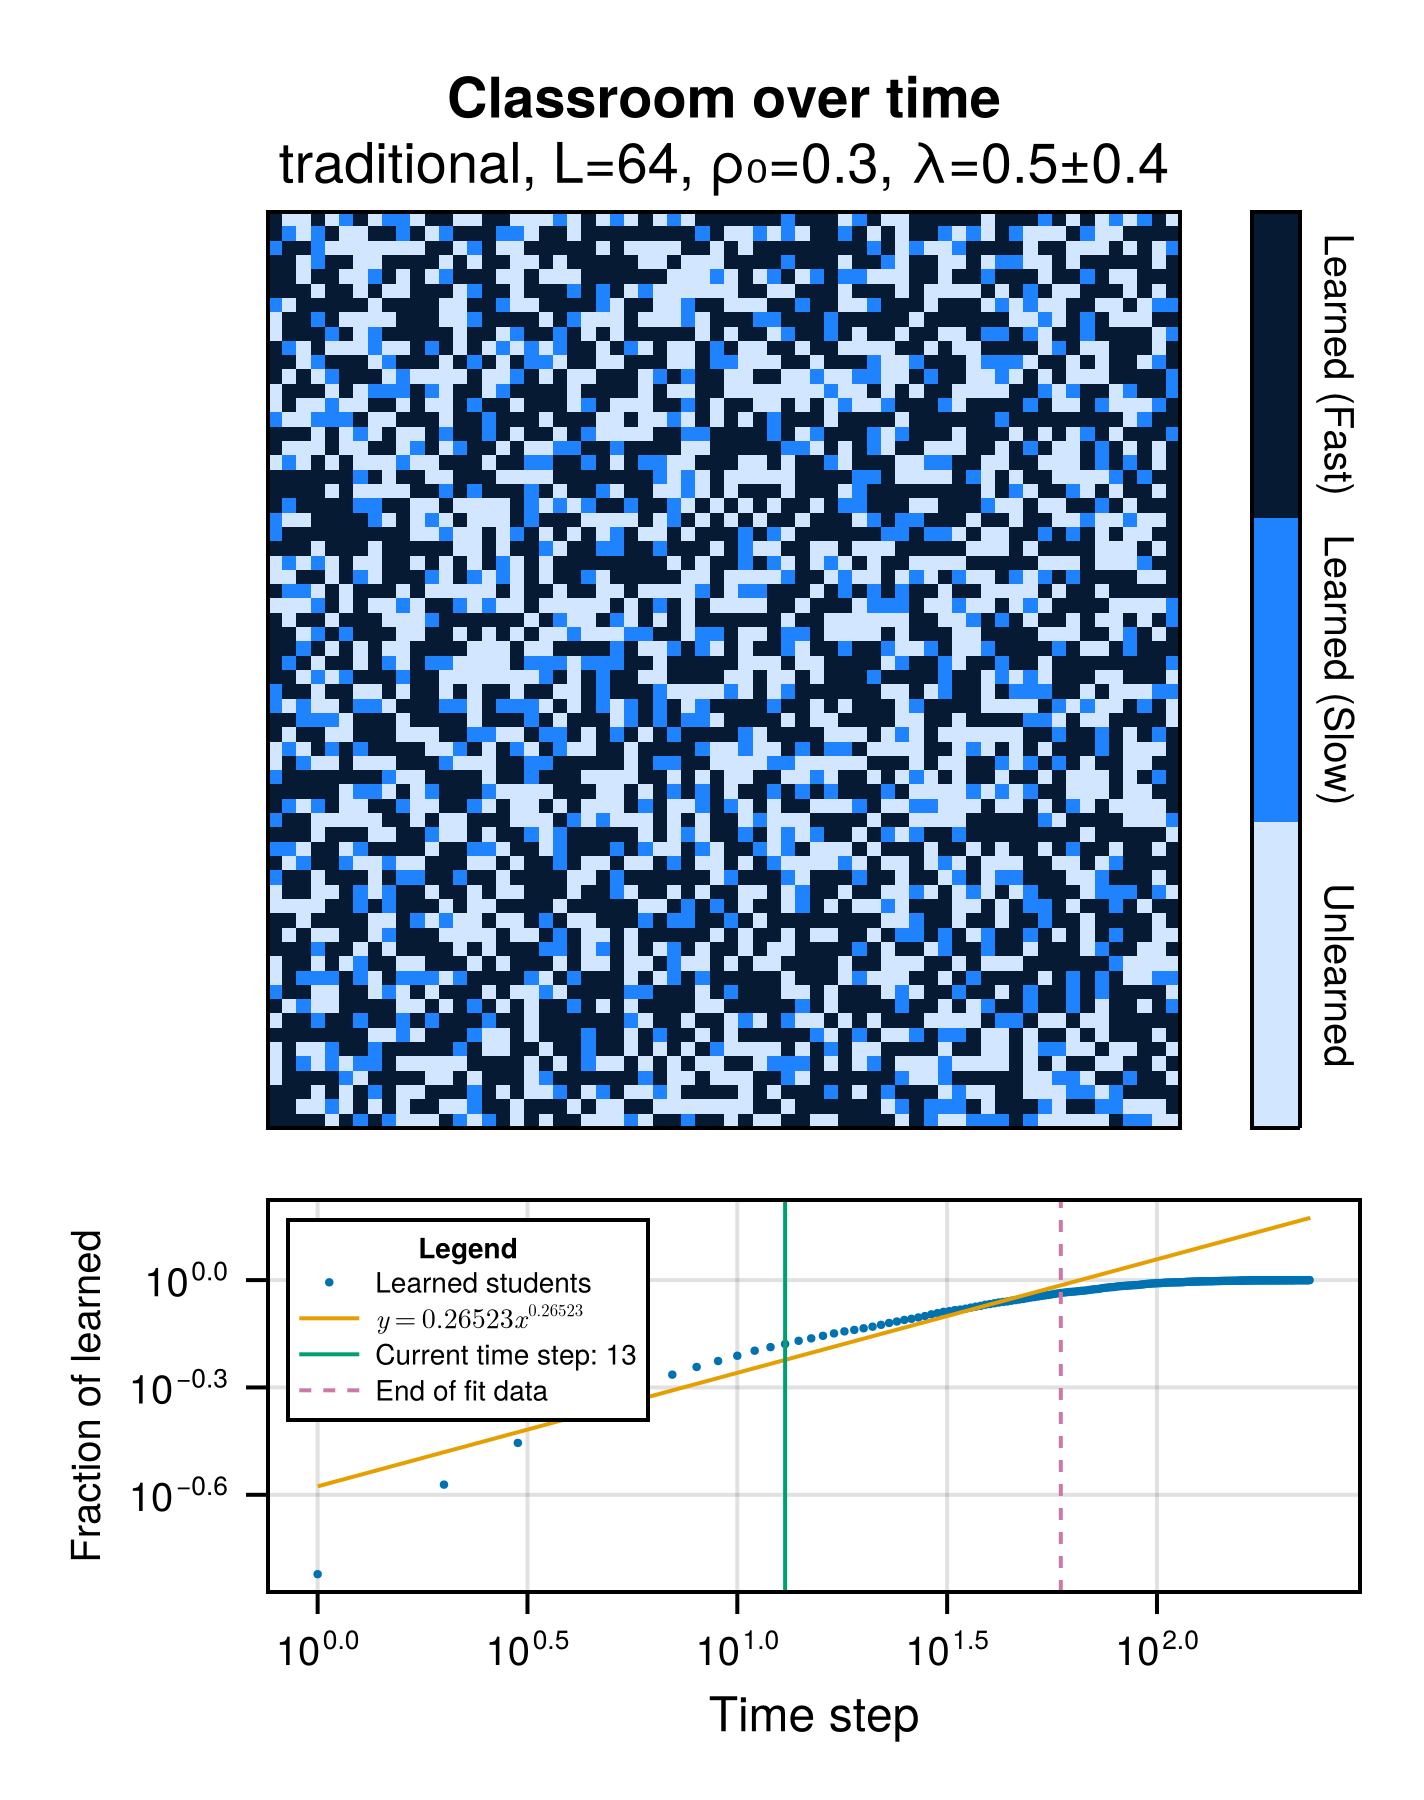
\includegraphics[width=0.40\textwidth]{figures/2D-BPCAIH-analysis/class evolutions/trad low rho high delta/2DBPCAIH-traditional-64-0.3-0.5-0.4-trial_3-13.png}}
   \subfigure[$t=50$]{\label{fig:2DBPCAIH class evolution trad low rho high delta 50}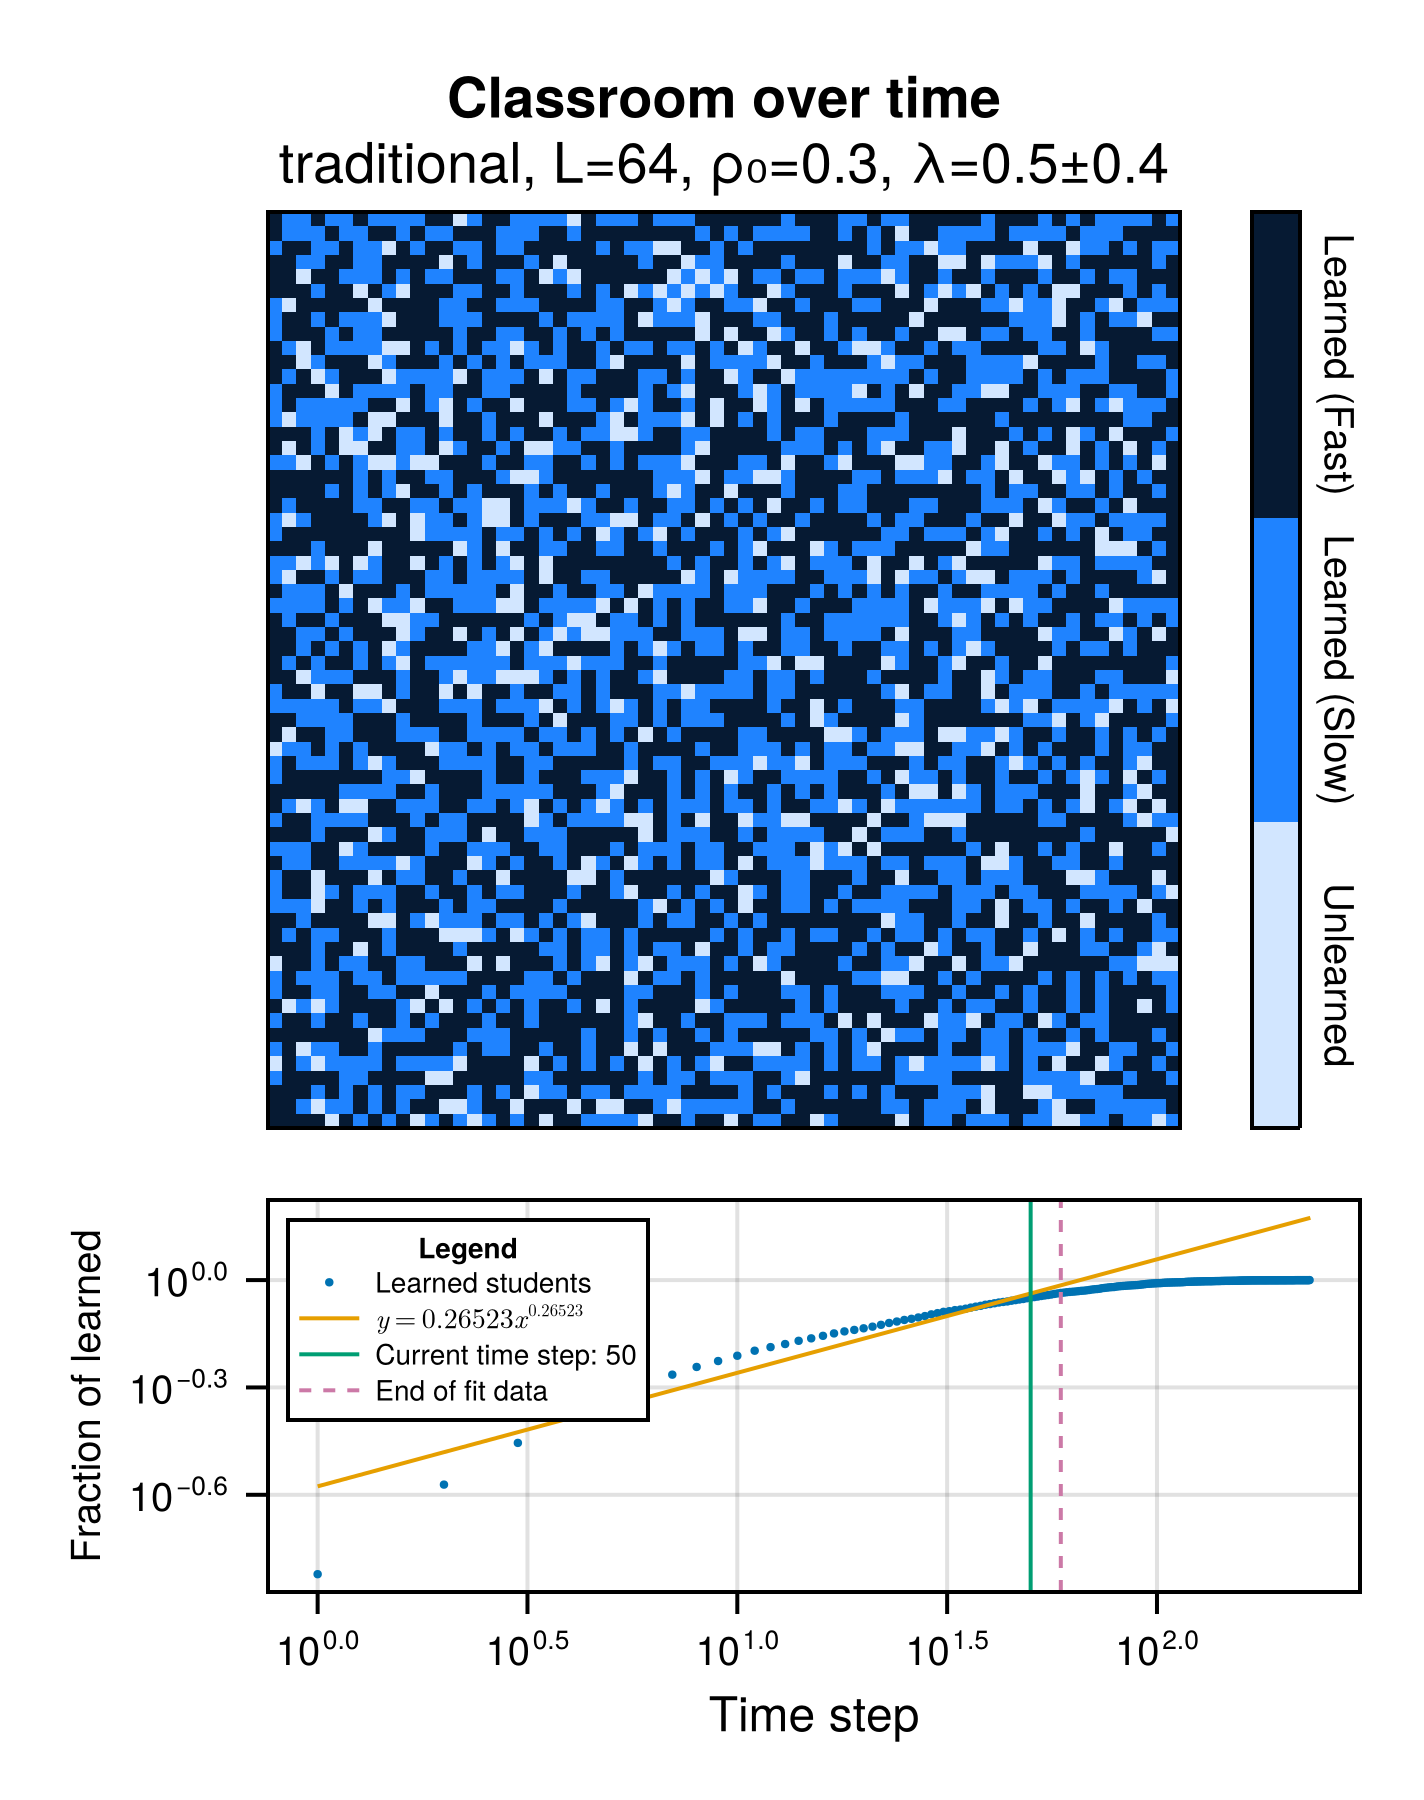
\includegraphics[width=0.40\textwidth]{figures/2D-BPCAIH-analysis/class evolutions/trad low rho high delta/2DBPCAIH-traditional-64-0.3-0.5-0.4-trial_3-50.png}}
   \subfigure[$t=80$]{\label{fig:2DBPCAIH class evolution trad low rho high delta 80}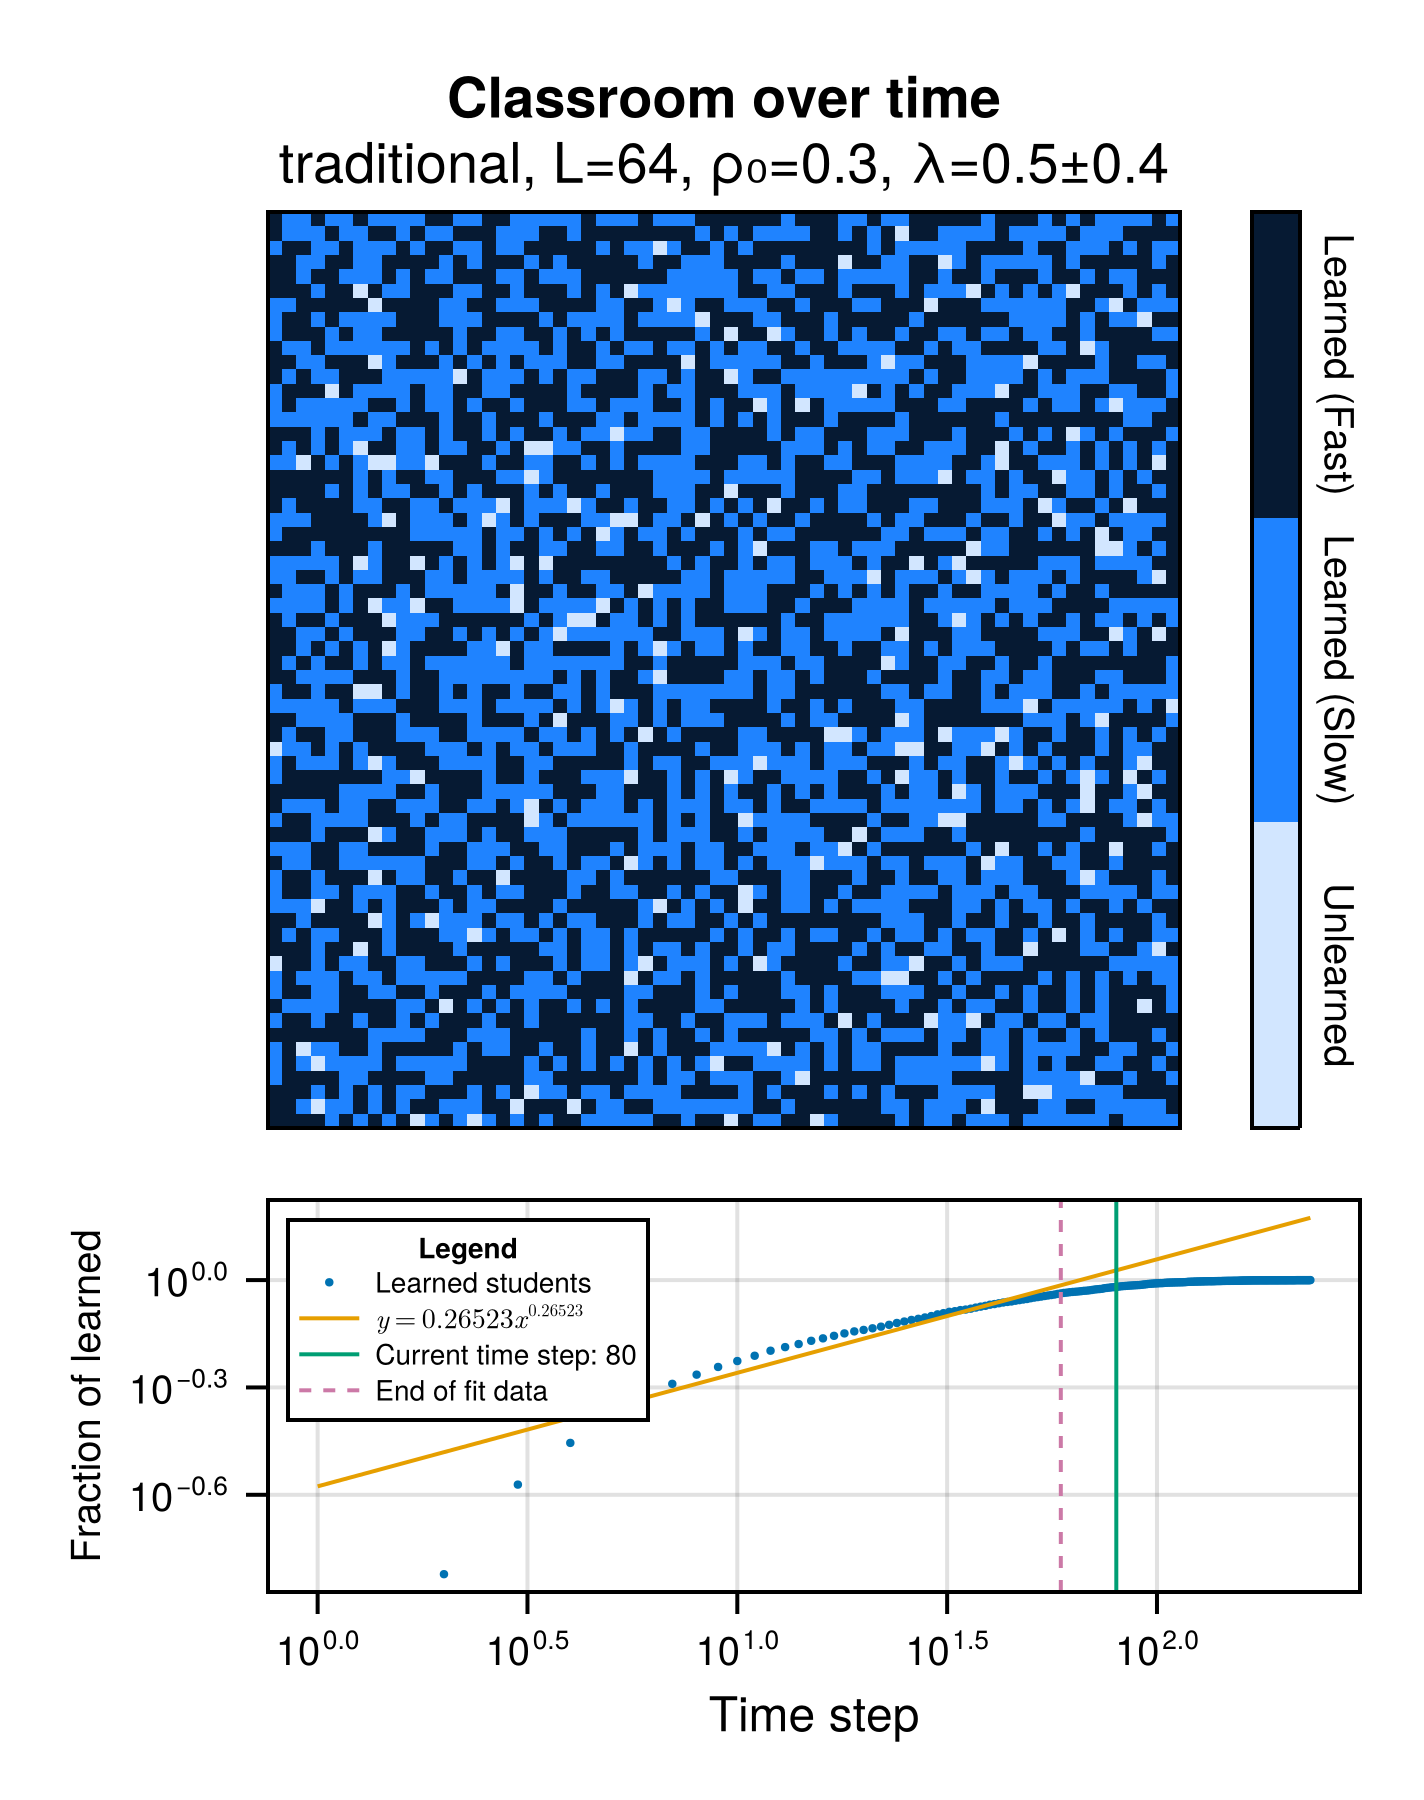
\includegraphics[width=0.40\textwidth]{figures/2D-BPCAIH-analysis/class evolutions/trad low rho high delta/2DBPCAIH-traditional-64-0.3-0.5-0.4-trial_3-80.png}}
   \caption[Example classroom evolution for the heterogeneous traditional instruction set up]{Sample classroom evolutions for PI with the inner corner SA with $L=128$ at different times $t$ for positional learning coefficient $\rho_0=0.9$, $\delta\lambda = 0.4$.
   Dark blue squares represent learned students with learning rate $\lambda = \lambda_0 + \delta\lambda$, blue squares represent learned students with learning rate $\lambda = \lambda_0 - \delta\lambda$, and light blue squares represent unlearned students.
   The accompanying graph shows the fraction of learned students as a function time step.
   The blue dots represent data points. 
   The yellow line shows the power law fit.
   The pink dashed vertical line shows where we truncate the data for fitting the power law.
   The green vertical line shows the current time step in the simulation.
   }
   \label{fig:2DBPCAIH sample class evolution trad low rho high delta}
\end{figure}

\subsection{Comparing temporal learning dynamics of different classroom configurations}

When varying the class size $N$, as in Figure~\ref{fig:2DBPCAIH t-learned size comparison}, we see that in traditional instruction, the dynamics remains generally unchanged, with only the time to learn $t_{max}$ increasing as the class size $N$ increases. 
For PI, an increase in class size $N$ adds a time delay to when the learning starts to speed up. 
Despite the added time delay, the general shape of the learning curve remains the same.
An increase in class size $N$ also does not affect the time to learn $t_{max}$ for PI as much as it does for the traditional model.

When varying the positional learning factor $\rho_0$, we see that it varies the shape of the learning curve for traditional instruction, especially for lower values of $\rho_0$ as shown in Figure~\ref{fig:2DBPCAIH t-learned rho comparison}. 
For traditional instruction, the value of $\rho_0$ also greatly changes the initial number of students that learn in the second time step.
The same figure shows that for PI, the value of $\rho_0$ has a similar effect to class size $N$, adding only a delay before learning accelerates.
Notably, the effect of $\rho_0$ is nonlinear for either instruction models.
We can see in the same figure that those with extremely low values of $\rho$, like that of $\rho_0=0.1$ perform much worse with the learning curves being further from $\rho_0=0.5$ than $\rho_0=0.9$.

Figure~\ref{fig:2DBPCAIH t-learned delta comparison} shows that an increase in heterogeneity $\delta\lambda$ changes how fast the slope of the learning curve changes for the traditional model without changing the initial number of learned students. 
As for PI, only very high $\delta\lambda$ values noticeably impact the learning curve.
The effect of heterogeneity for PI is also similar to the effects of class size $N$ and positional learning factor $\rho_0$ where it only adds a time delay, shifting the learning curve to the right.

As shown in Figure~\ref{fig:2DBPCAIH t-learned SA comparison}, when comparing between the different SA's for PI and traditional instruction, at least for $L=64, \rho_0=0.5, \lambda=0.5\pm0.2$, traditional instruction generally performs better than PI, especially in the early time steps. 
Among the different SA's for PI, the inner corner SA still performs the best while the center and outer corner SAs perform similarly, the same conclusion we got from the homogenous case.
Contrary to the results of the homogenous classes, the random SA performed better than the center and outer corner SAs.

One observation that is consistent with all the comparisons shown in Figure~\ref{fig:2DBPCAIH t-learned comparisons} is that even though using traditional instruction has more students learning in the early time steps, it also spends more time waiting for the last few students to learn. 
In contrast, PI setups take some time for learning to accelerate, but once the majority learn, the remaining students quickly follow regardless of their individual learning rate.
This makes PI have a shorter time to learn $t_{max}$, despite being outperformed by the traditional model in early time steps.
This phenomenon is further investigated in the next sections where we look closer at the different factors that can affect which set up is better for different classroom parameters.

\begin{figure}[htbp!]
   \centering
   \subfigure[Size comparison]{\label{fig:2DBPCAIH t-learned size comparison}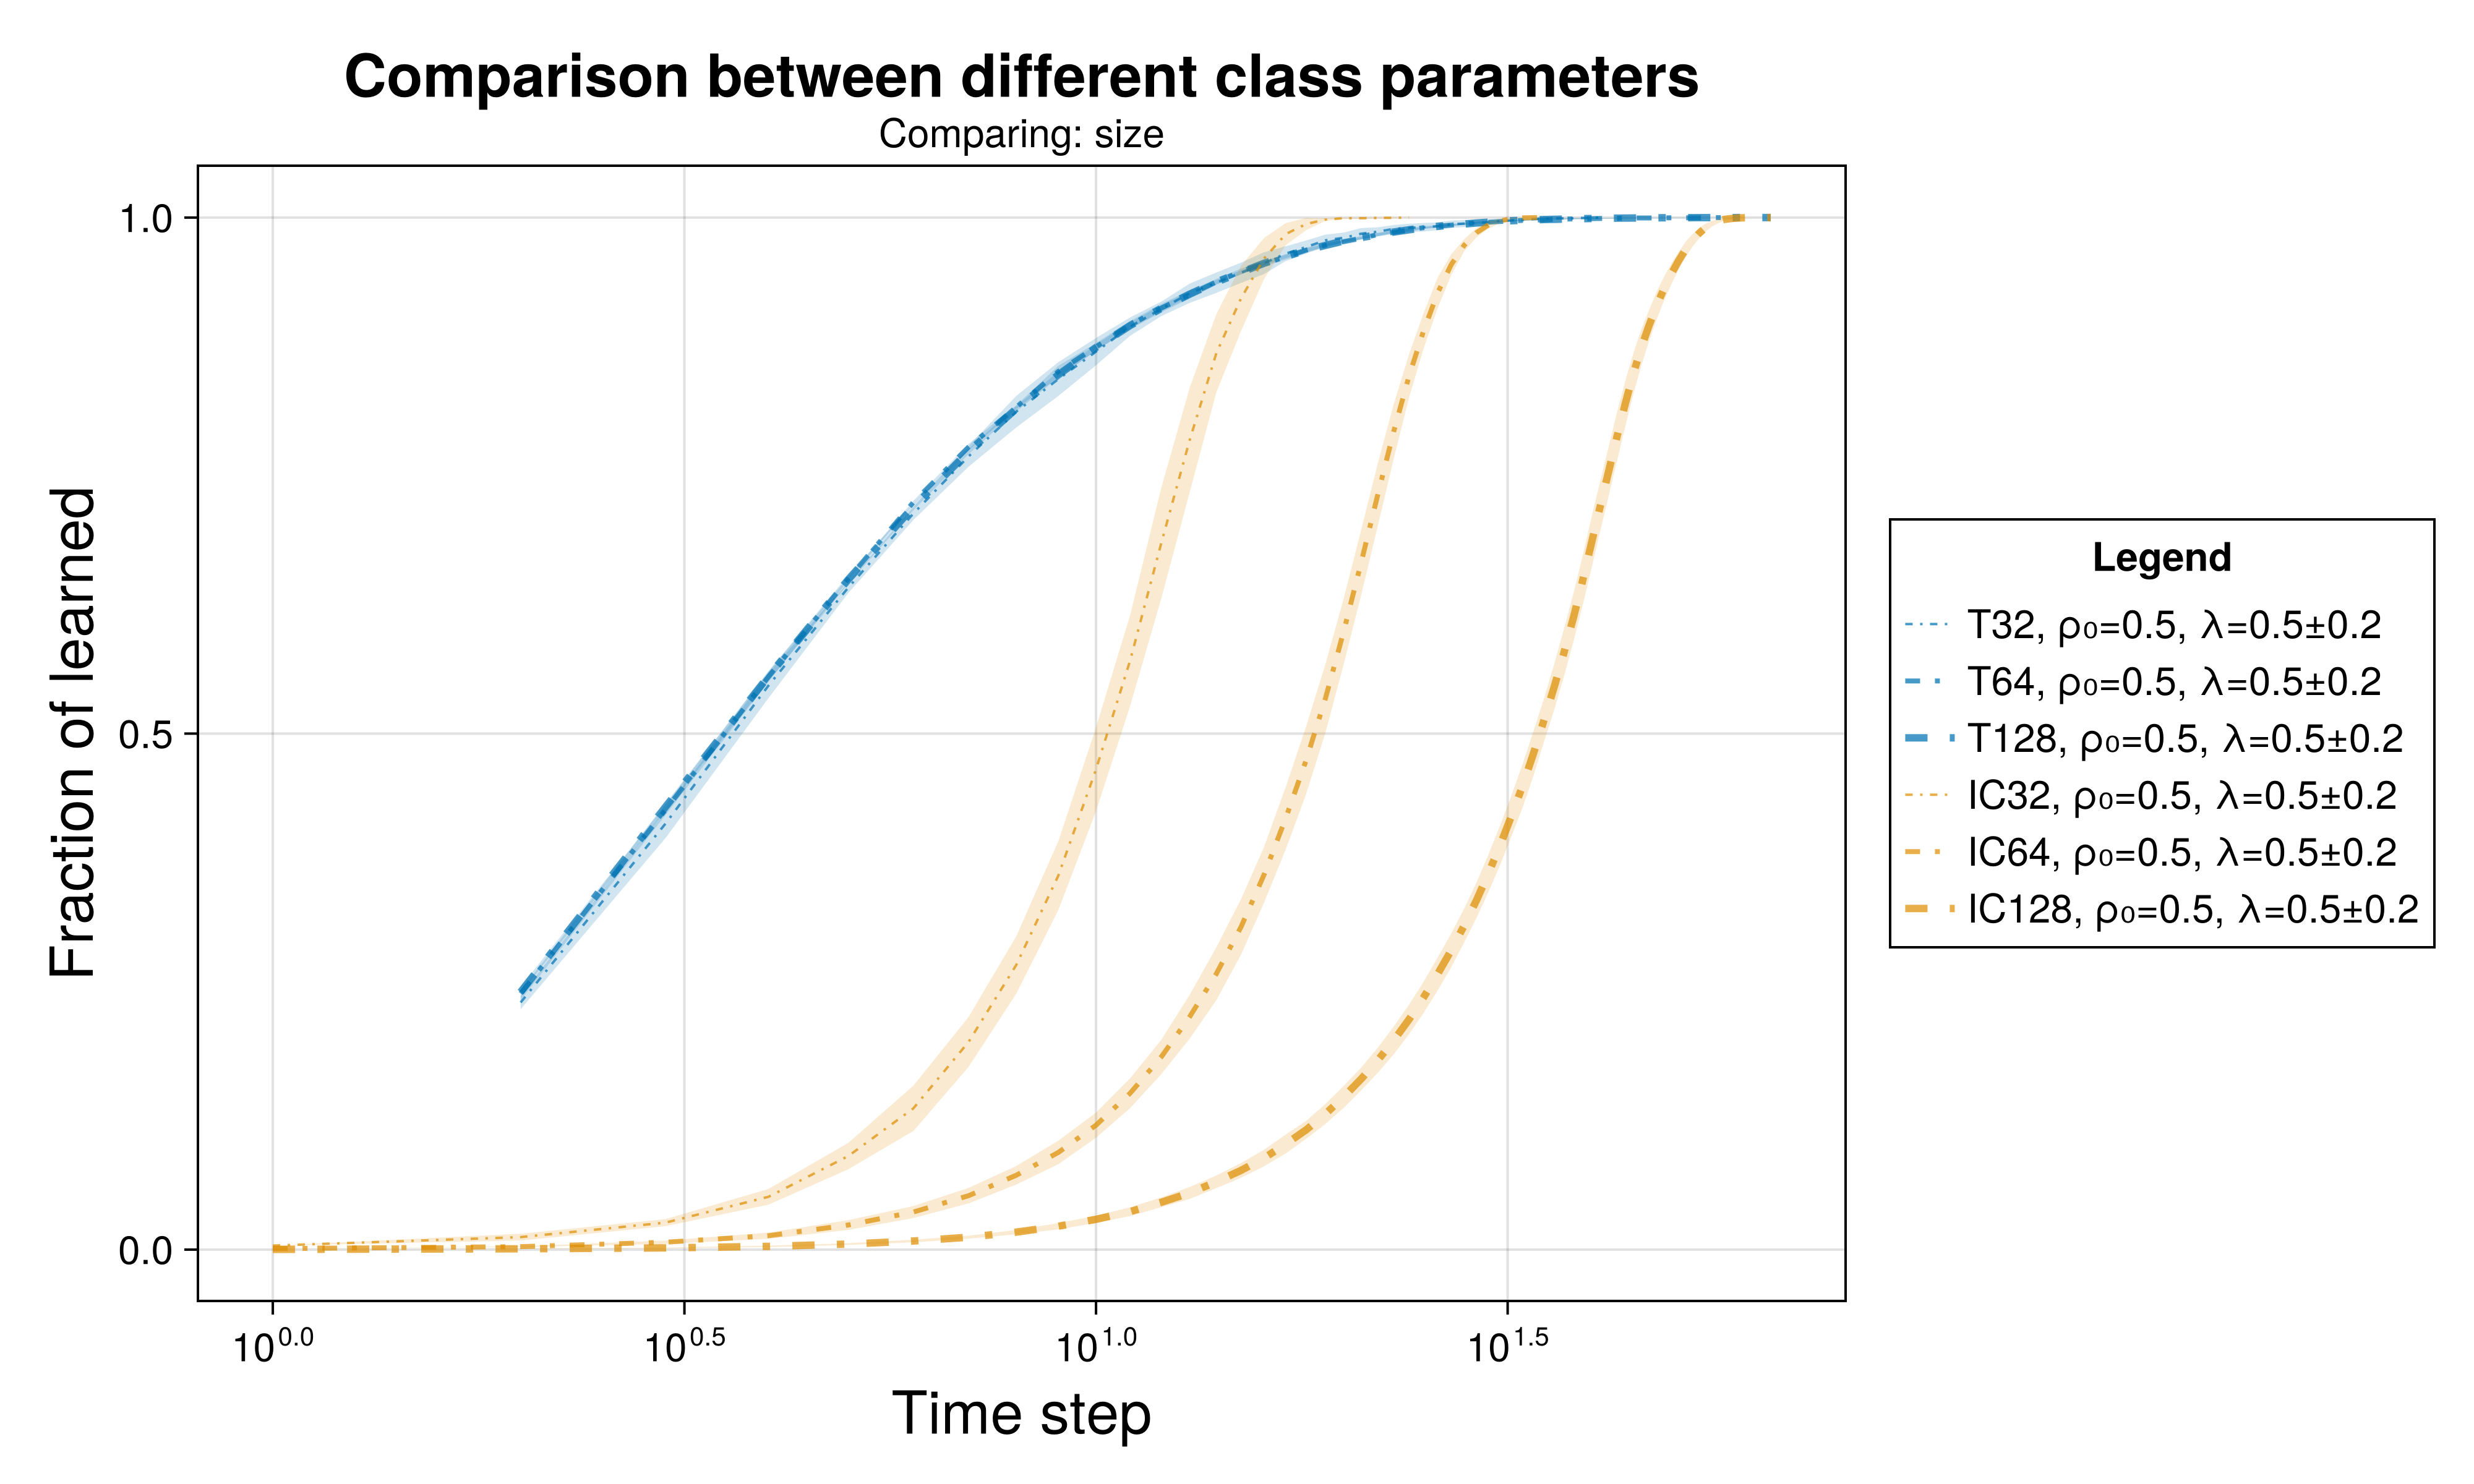
\includegraphics[width=0.49\textwidth]{figures/2D-BPCAIH-analysis/comparison plots/size.png}}
   \subfigure[$\rho_0$ comparison]{\label{fig:2DBPCAIH t-learned rho comparison}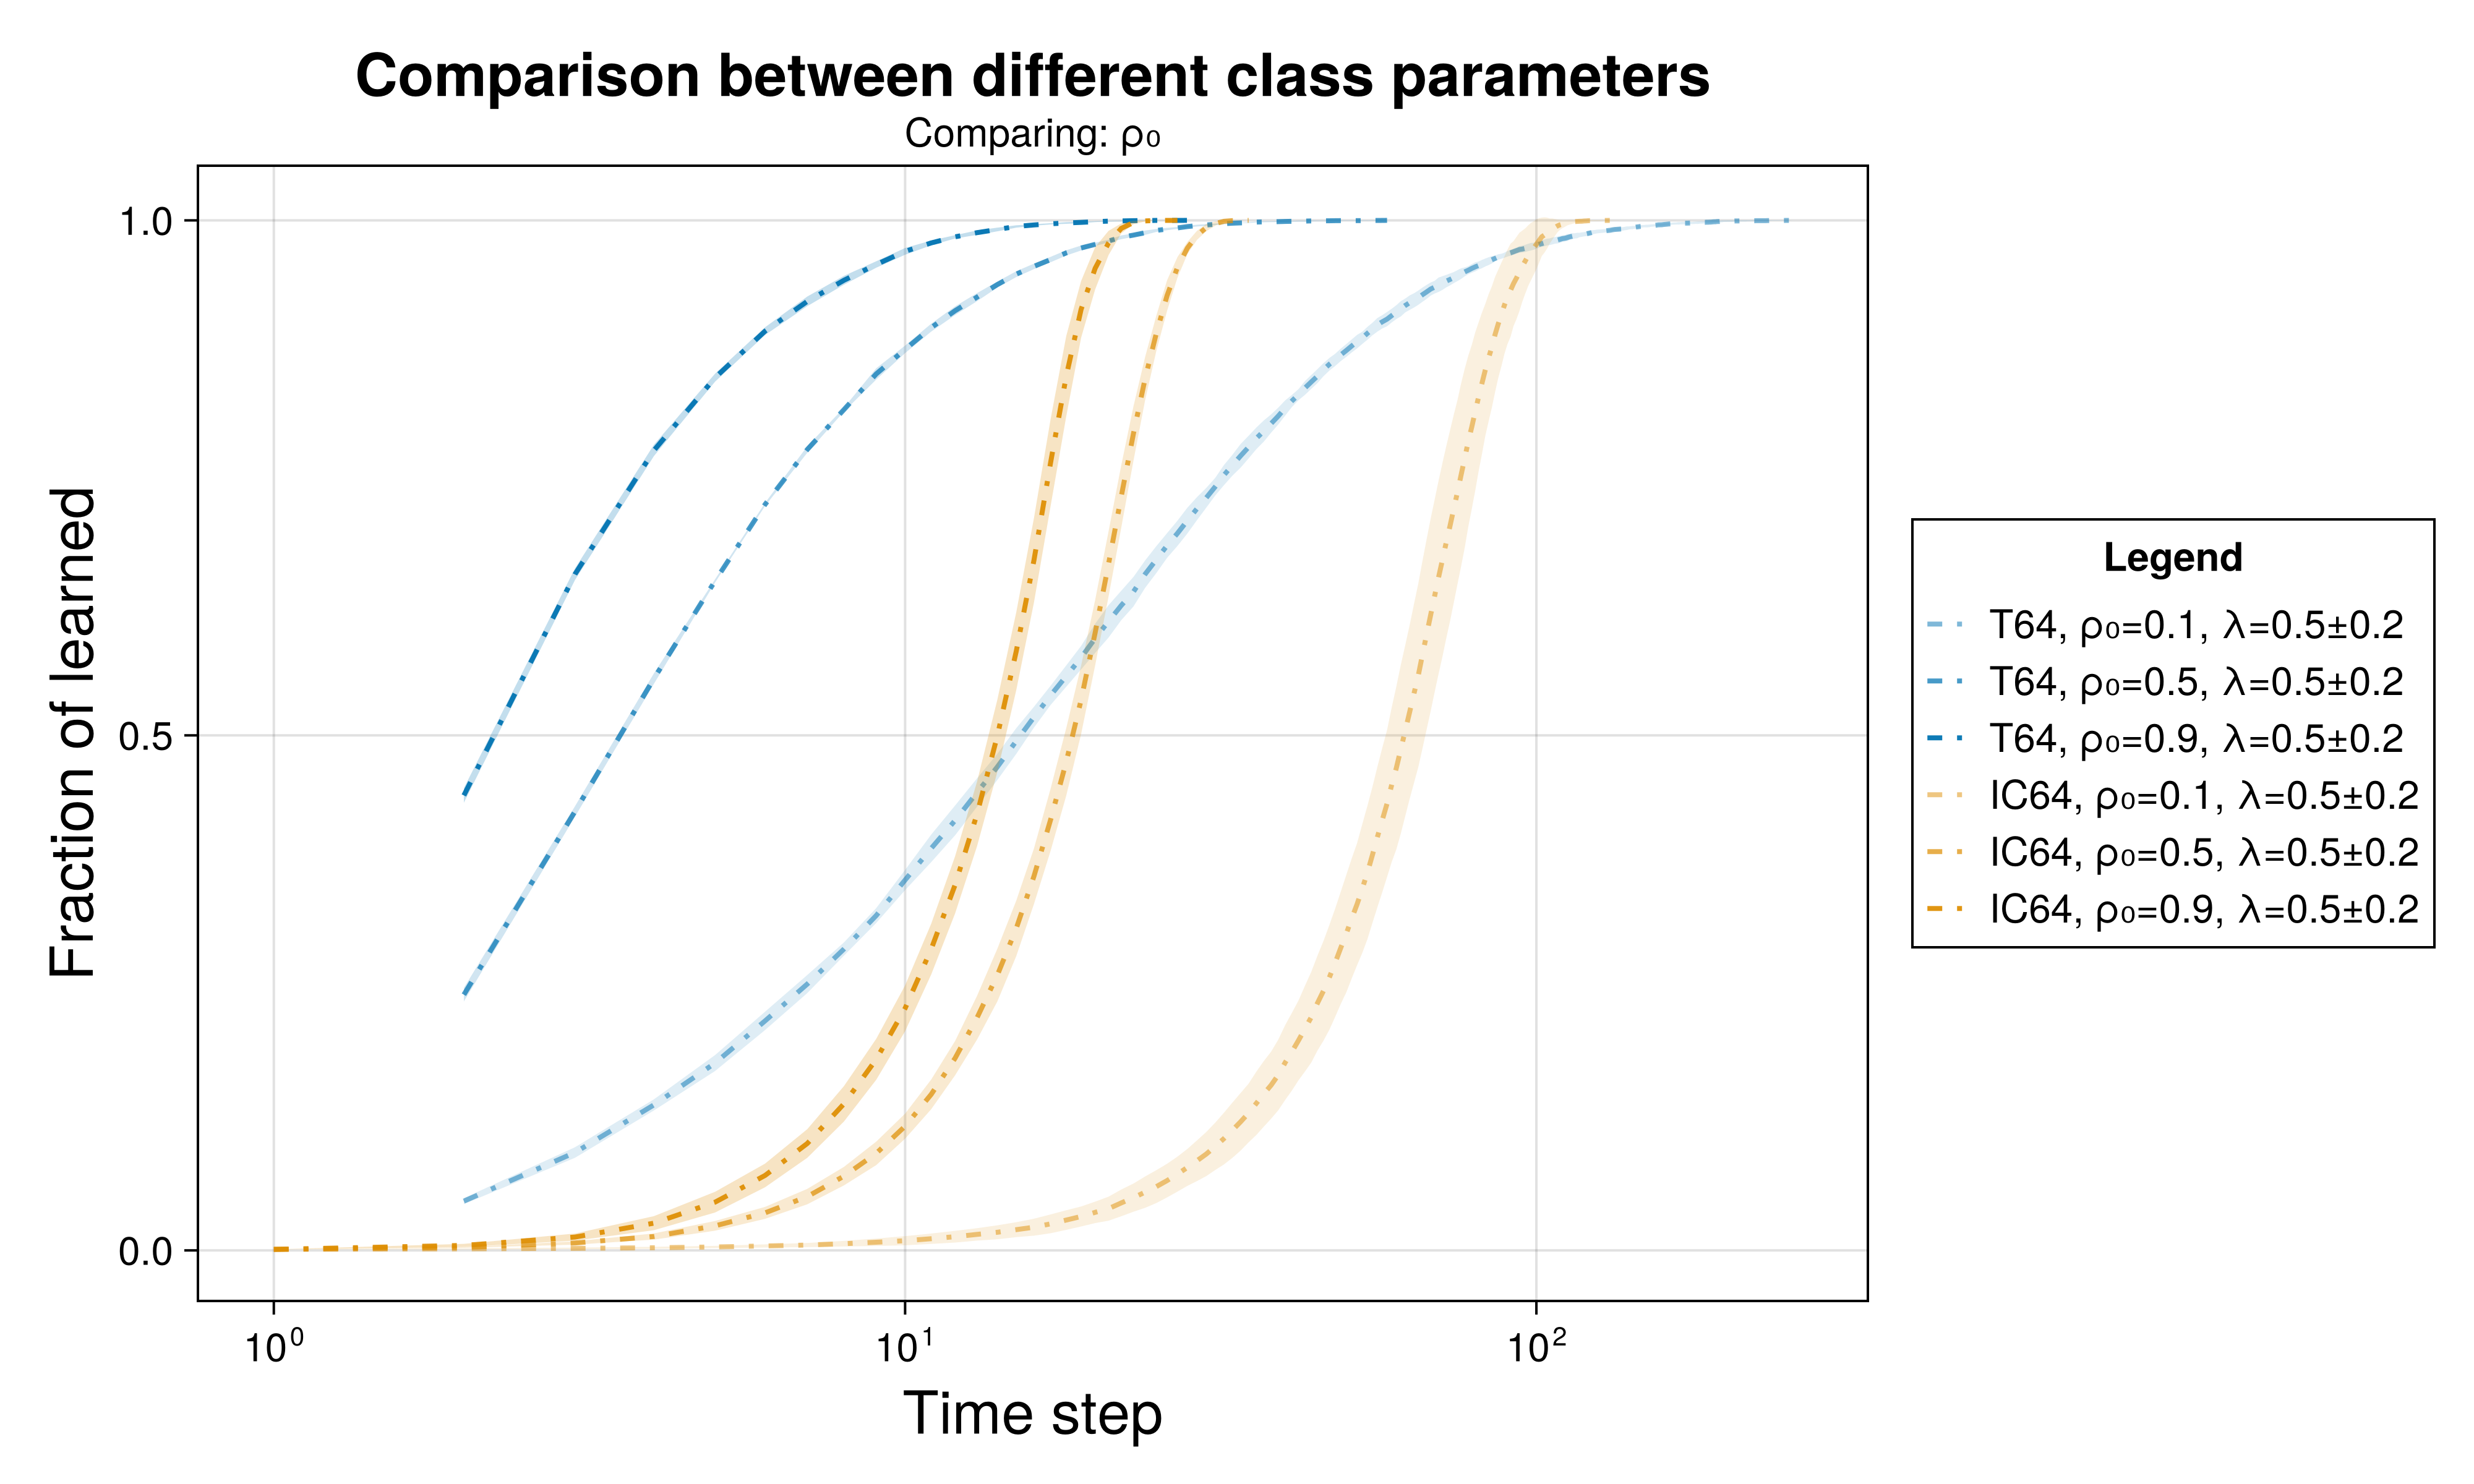
\includegraphics[width=0.49\textwidth]{figures/2D-BPCAIH-analysis/comparison plots/ρ₀.png}}
   \subfigure[$\delta\lambda$ comparison]{\label{fig:2DBPCAIH t-learned delta comparison}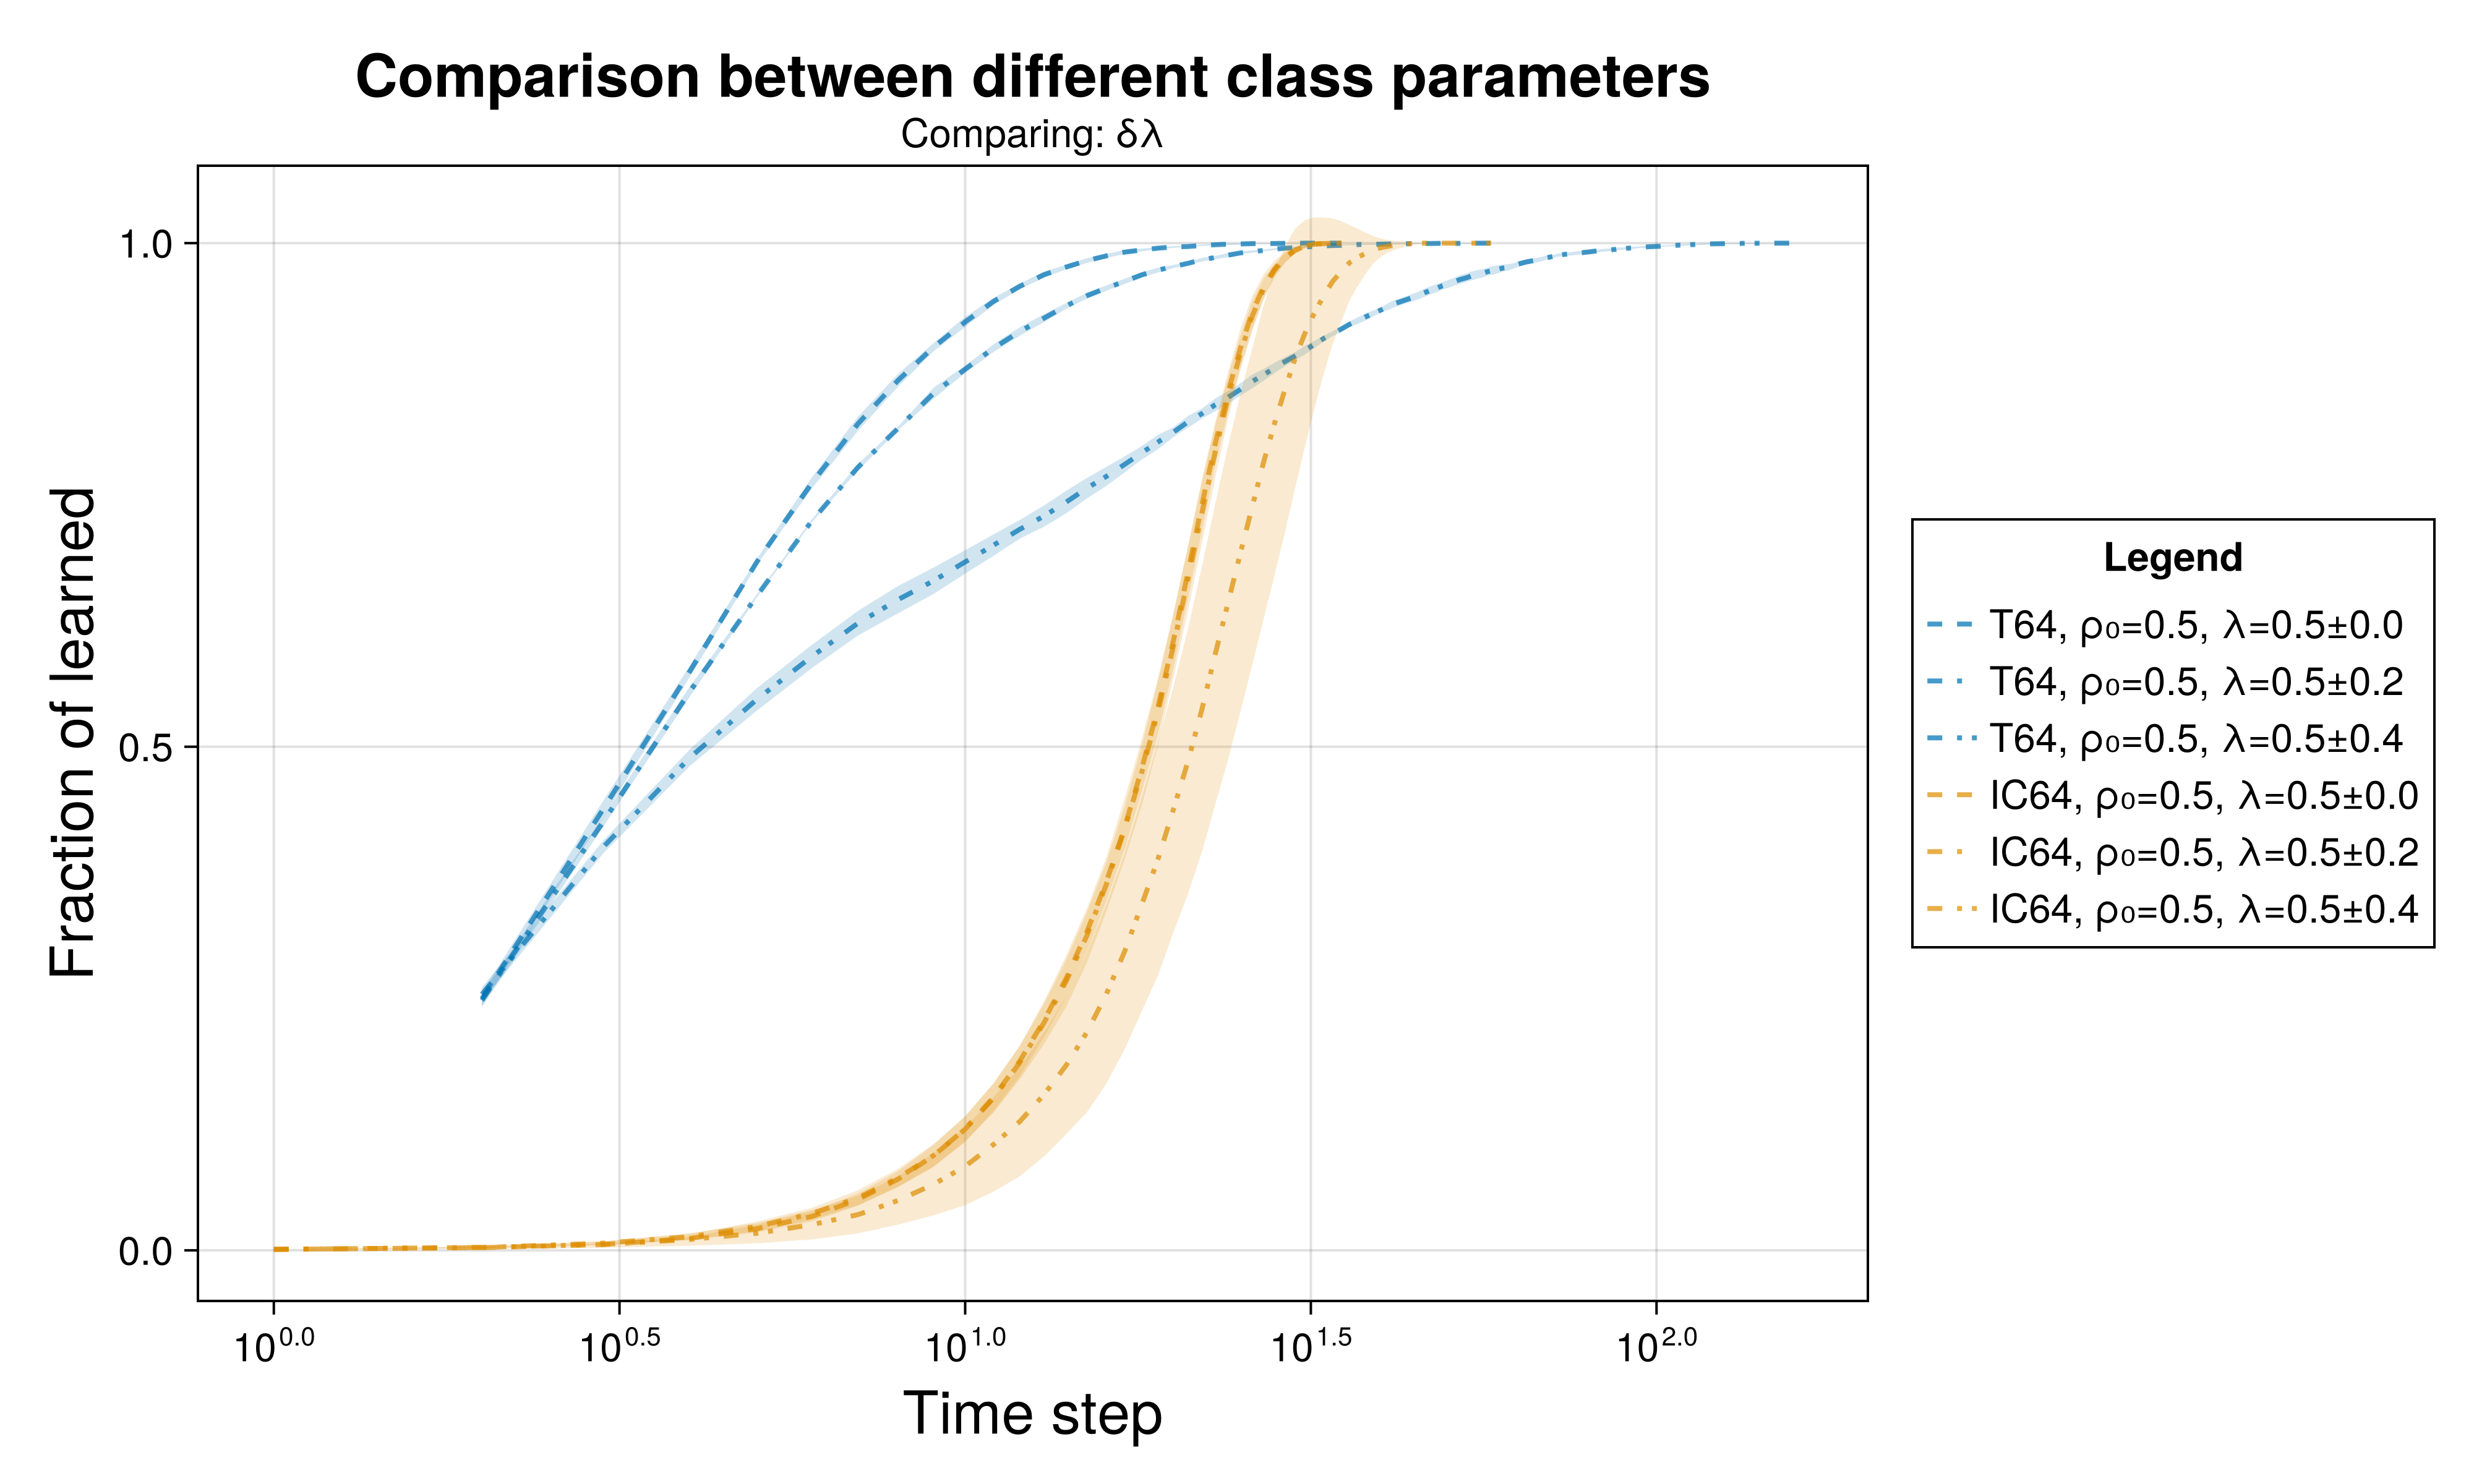
\includegraphics[width=0.49\textwidth]{figures/2D-BPCAIH-analysis/comparison plots/δλ.png}}
   \subfigure[SA comparison]{\label{fig:2DBPCAIH t-learned SA comparison}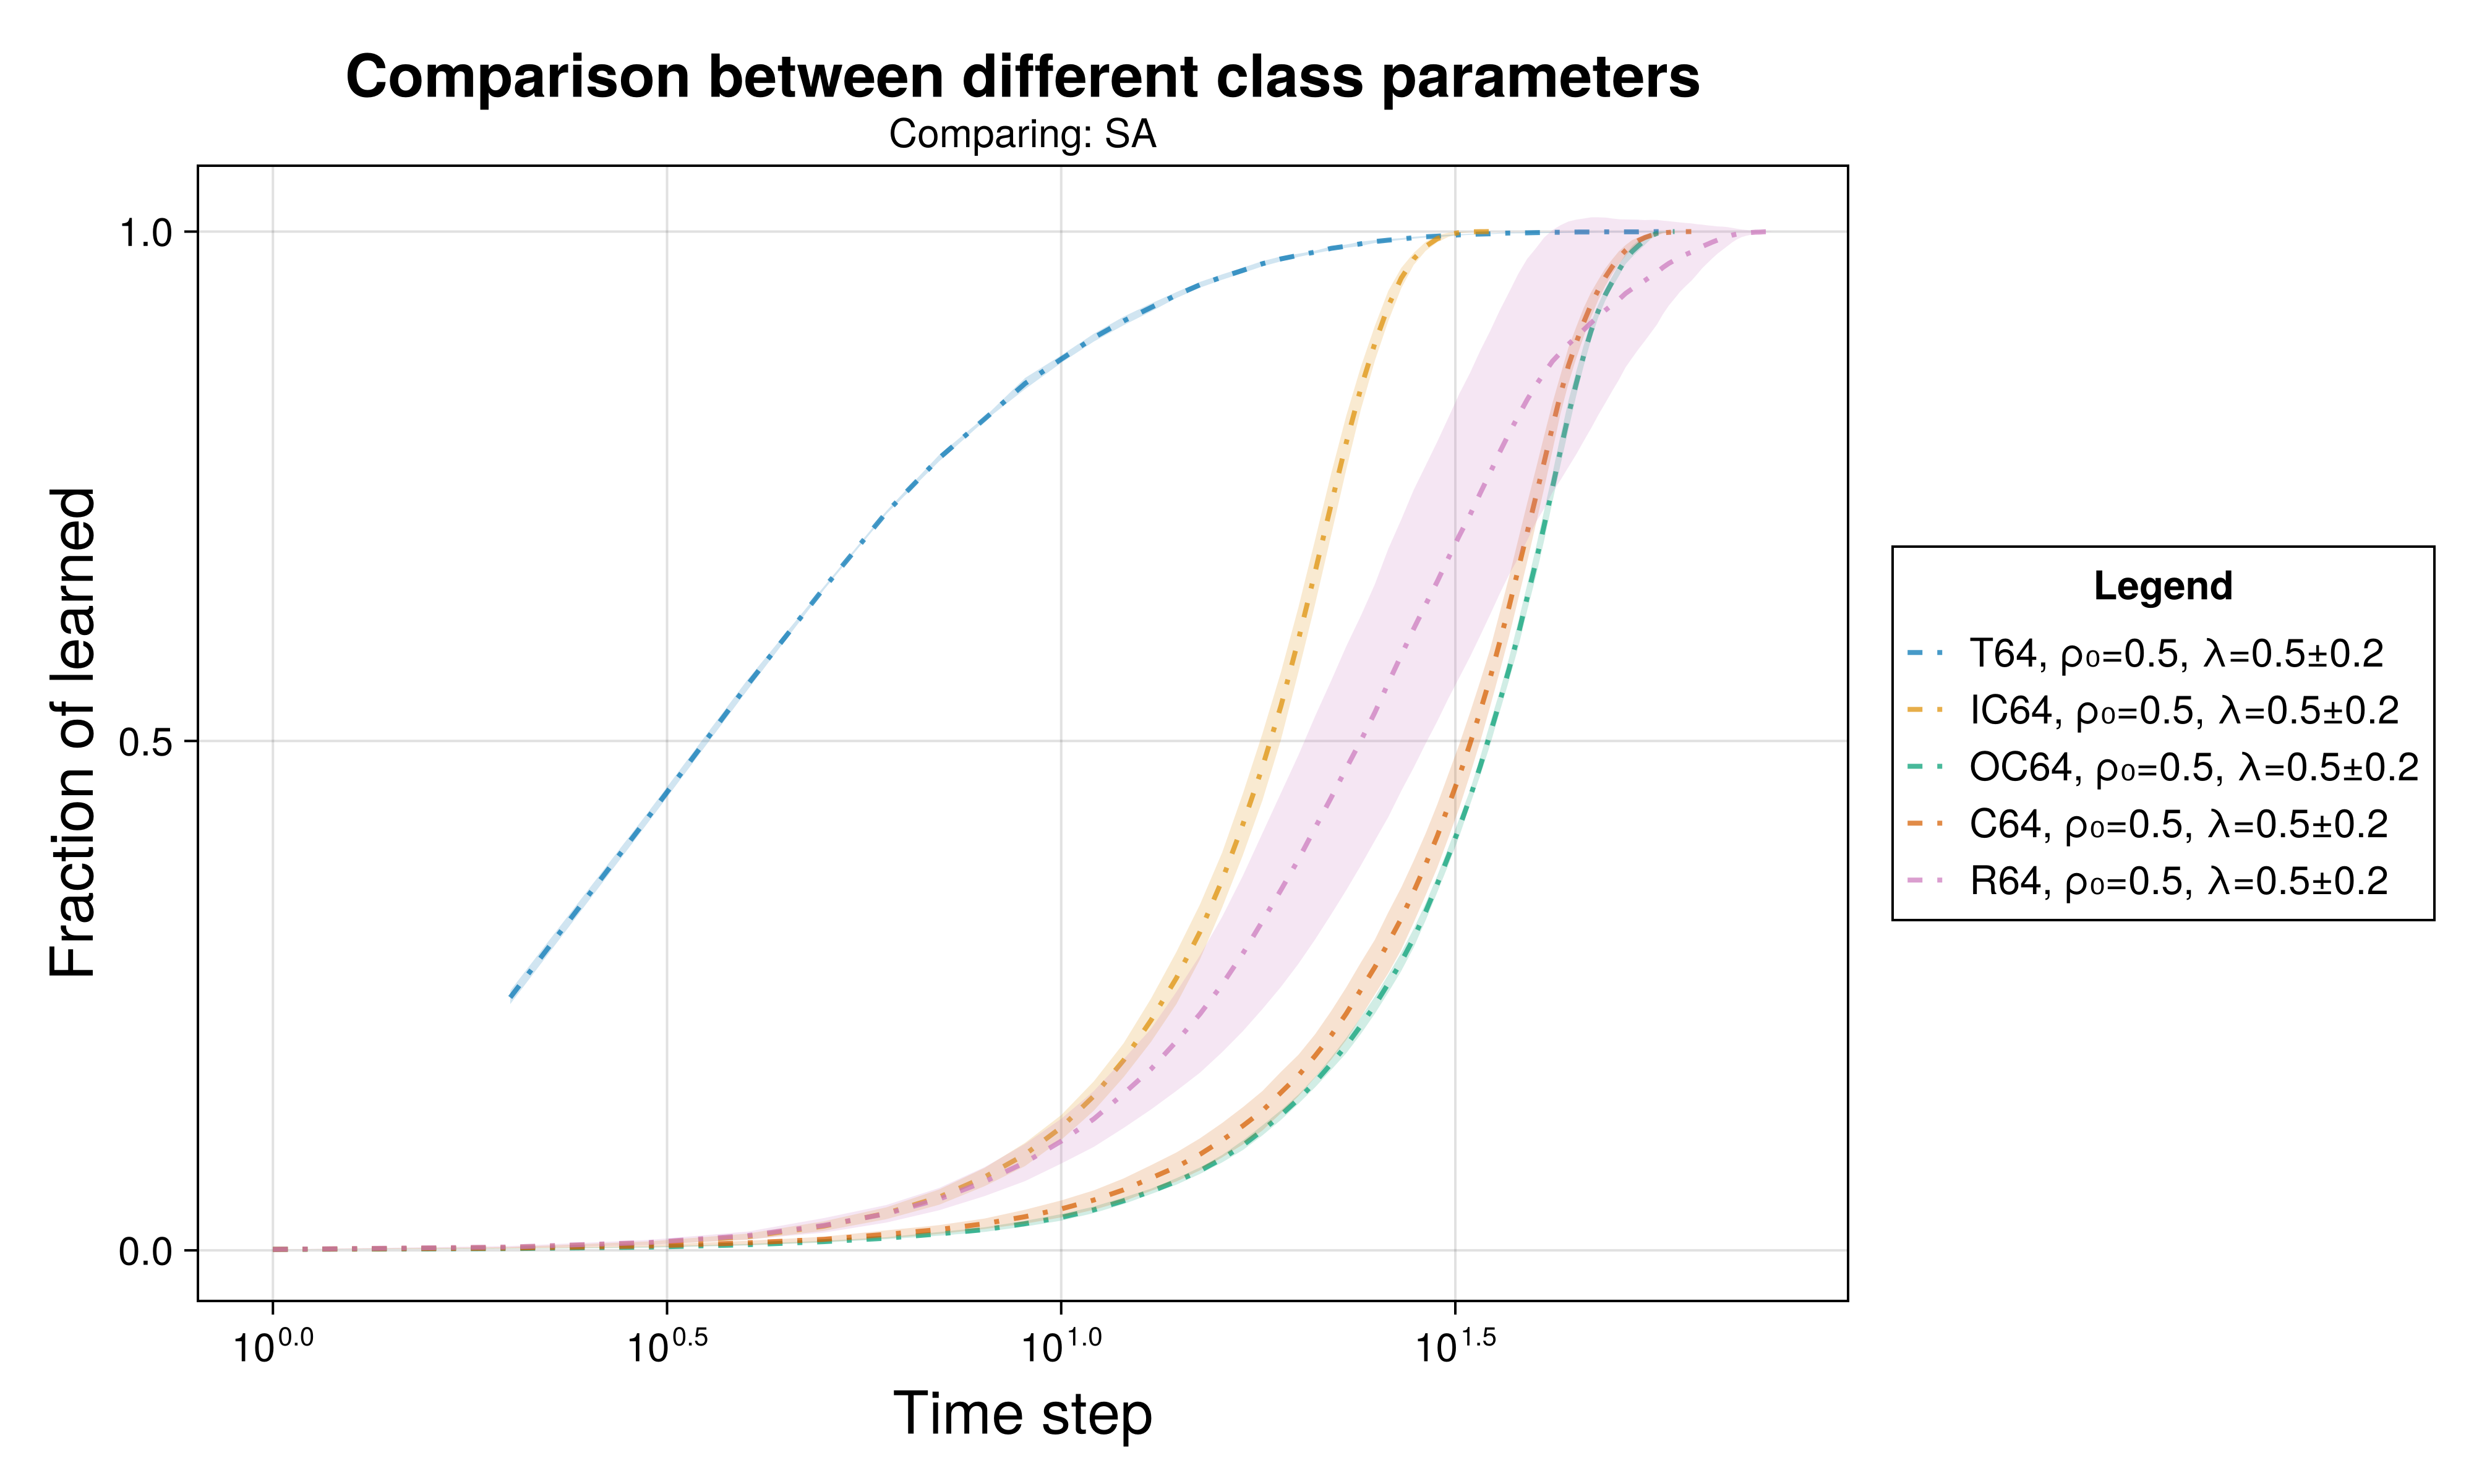
\includegraphics[width=0.49\textwidth]{figures/2D-BPCAIH-analysis/comparison plots/SA.png}}
   \caption[Comparison of time to learn $t_{max}$ and fraction of learned students $f$ for different representative heterogeneous classroom configurations]{Comparison of time to learn $t_{max}$ and fraction of learned students for different representative classroom configurations. 
   Each SA corresponds to a different color, blue for traditional, yellow for inner corner, green for outer corner, orange for center, and pink for random. 
   Different values $\rho_0$ corresponds to varying alpha or transparency, where lower $\rho_0$ values are more transparent.
   Different values of $\delta\lambda$ corresponds to different line styles, where $\delta\lambda=0.0$ are represented by dashed lines, $\delta\lambda=0.2$ are represented by lines with alternating dots and dashes, $\delta\lambda=0.4$ are represented by two dots followed by a dash.
   Different classroom sizes $L$ corresponds to different line widths, where bigger classroom sizes correspond to thicker lines.
   The bands around each line show the standard deviation of the data over 5 trials.
   Higher fraction of learned indicates better performance.
   }
   \label{fig:2DBPCAIH t-learned comparisons}
\end{figure}

\newpage % new page after section class evolution

\section{Class learning rate $m$ vs positional learning factor $\rho_0$}\label{sec:BPCAIH m vs rho}

Figure~\ref{fig:2DBPCAIH m rho plot} shows that class learning rate becomes inconsistent with the positional learning factor $\rho_0$ in PI models when introducing heterogeneity. 
The inconsistency may be caused by sampling problem where the first 50\% of the data may not be just capturing the initial dynamics of the classroom, which should be the only basis of the class learning rate $m$.
With heterogeneity, PI models no longer show trends in learning rate $m$ as a function of positional learning factor $\rho_0$.

The traditional instruction model shows a similar trend in learning rate $m$ as with time to learn $t_{max}$ where homogenous classrooms perform better than heterogeneous classrooms.
This might be explained by the spatio-temporal dynamics of traditional learning models where the fast learning students learn first, and the slow learning students learn last, as discussed in Section \ref{sec:BPCAIH effects on classroom evolution} and shown in Figure~\ref{fig:2DBPCAIH sample class evolution trad low rho high delta}.

Moving forward, we will only focus on the time to learn $t_{max}$ as a metric for performance.

\begin{figure}[htbp!]
   \centering
   \subfigure[Center $L=32$]{\label{fig:BPCAIH m plot C32}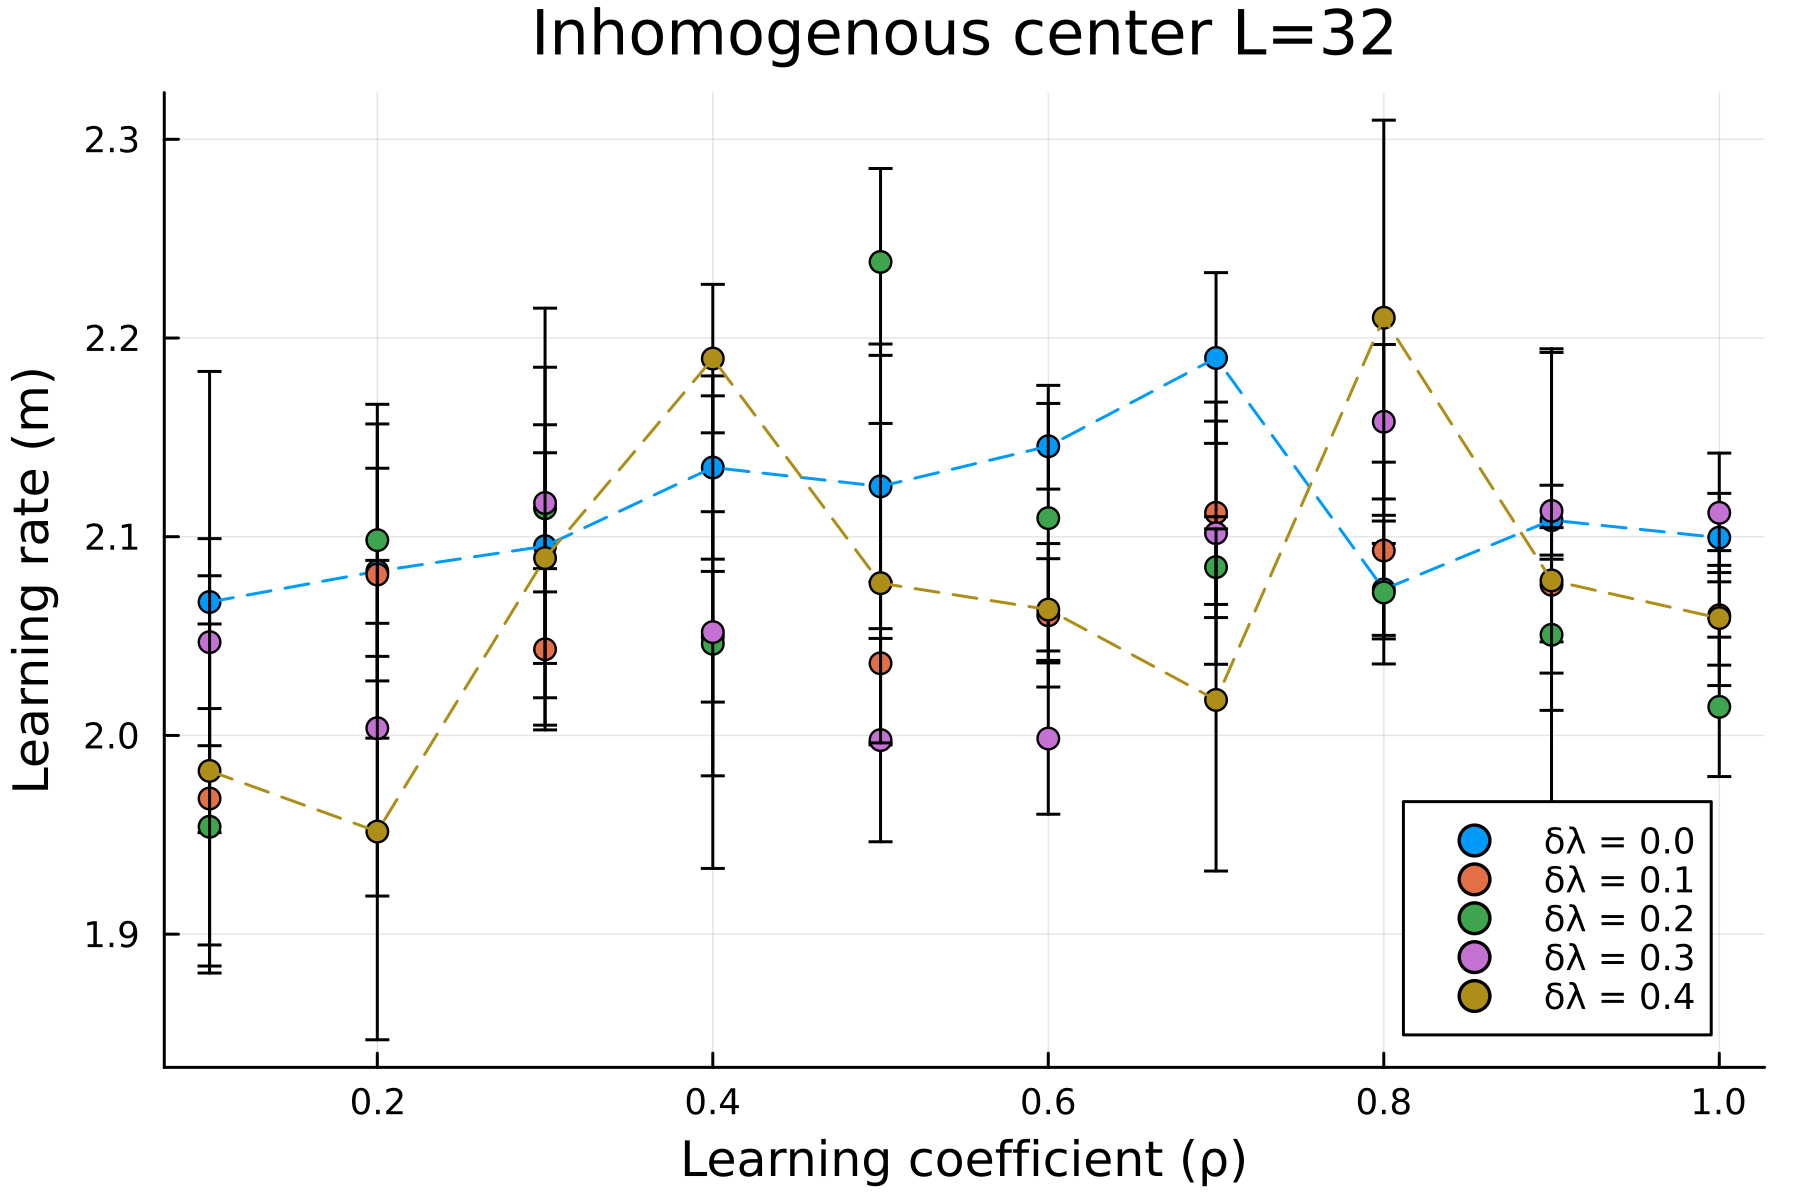
\includegraphics[width=0.40\textwidth]{figures/2D-BPCAIH-analysis/m-plots/m-center-32.png}}
   \subfigure[Outer corner $L=48$]{\label{fig:BPCAIH m plot O48}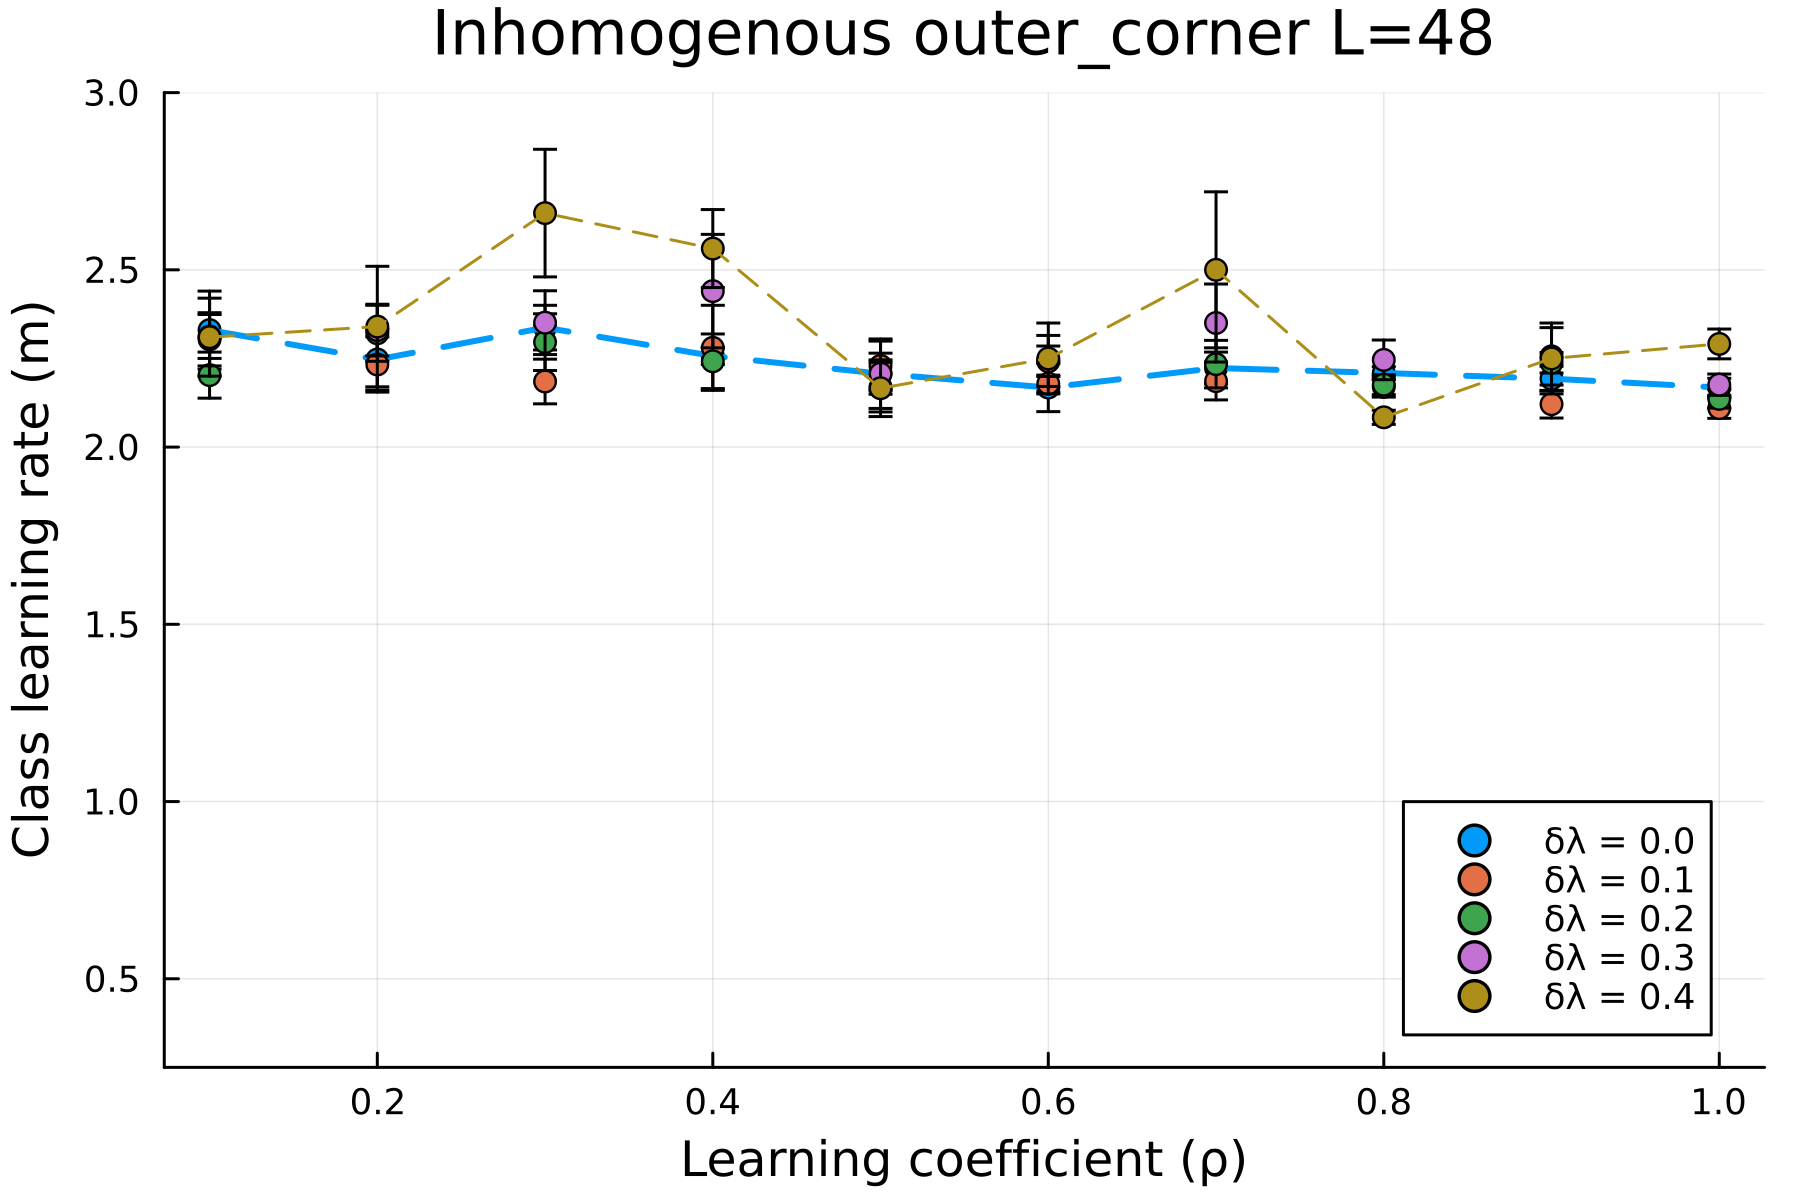
\includegraphics[width=0.40\textwidth]{figures/2D-BPCAIH-analysis/m-plots/m-outer_corner-48.png}}
   \subfigure[Inner corner $L=64$]{\label{fig:BPCAIH m plot I64}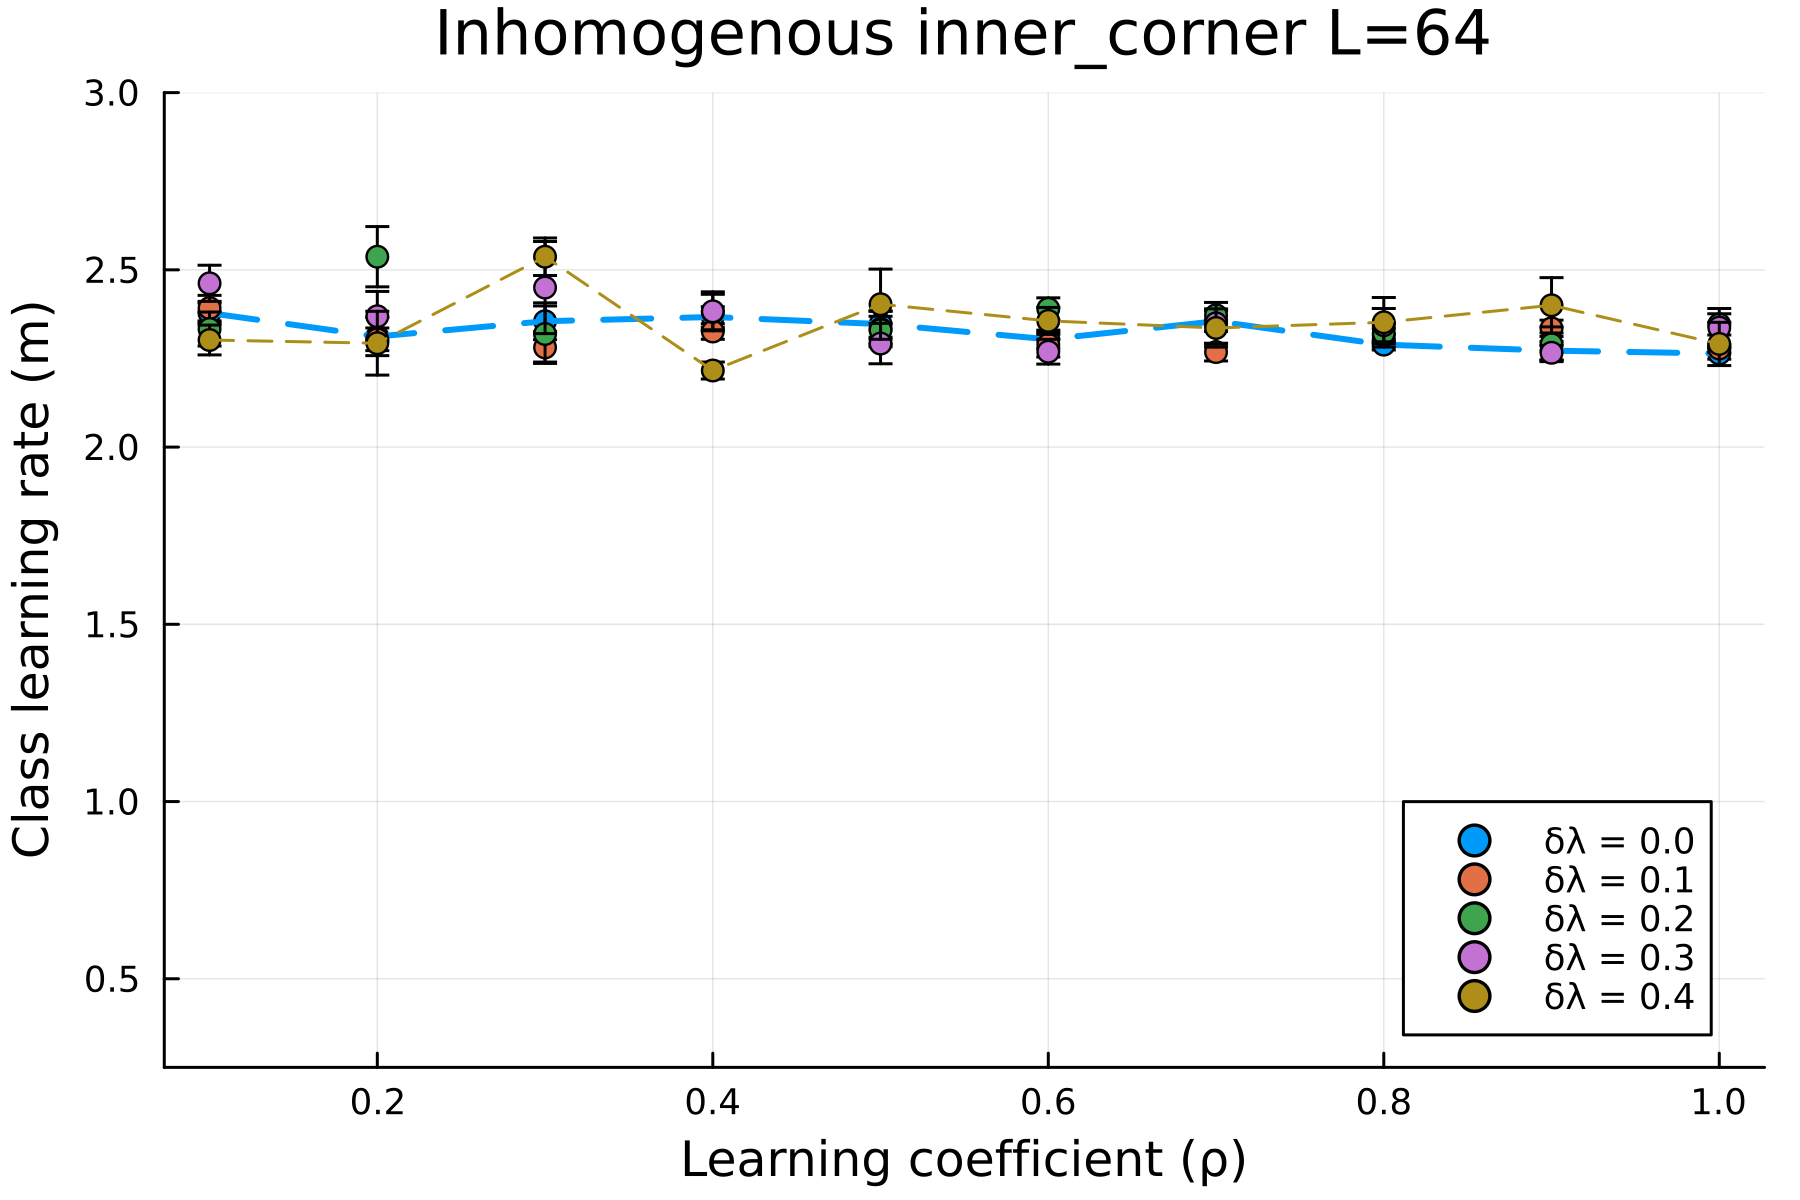
\includegraphics[width=0.40\textwidth]{figures/2D-BPCAIH-analysis/m-plots/m-inner_corner-64.png}}
   \subfigure[Random $L=96$]{\label{fig:BPCAIH m plot R96}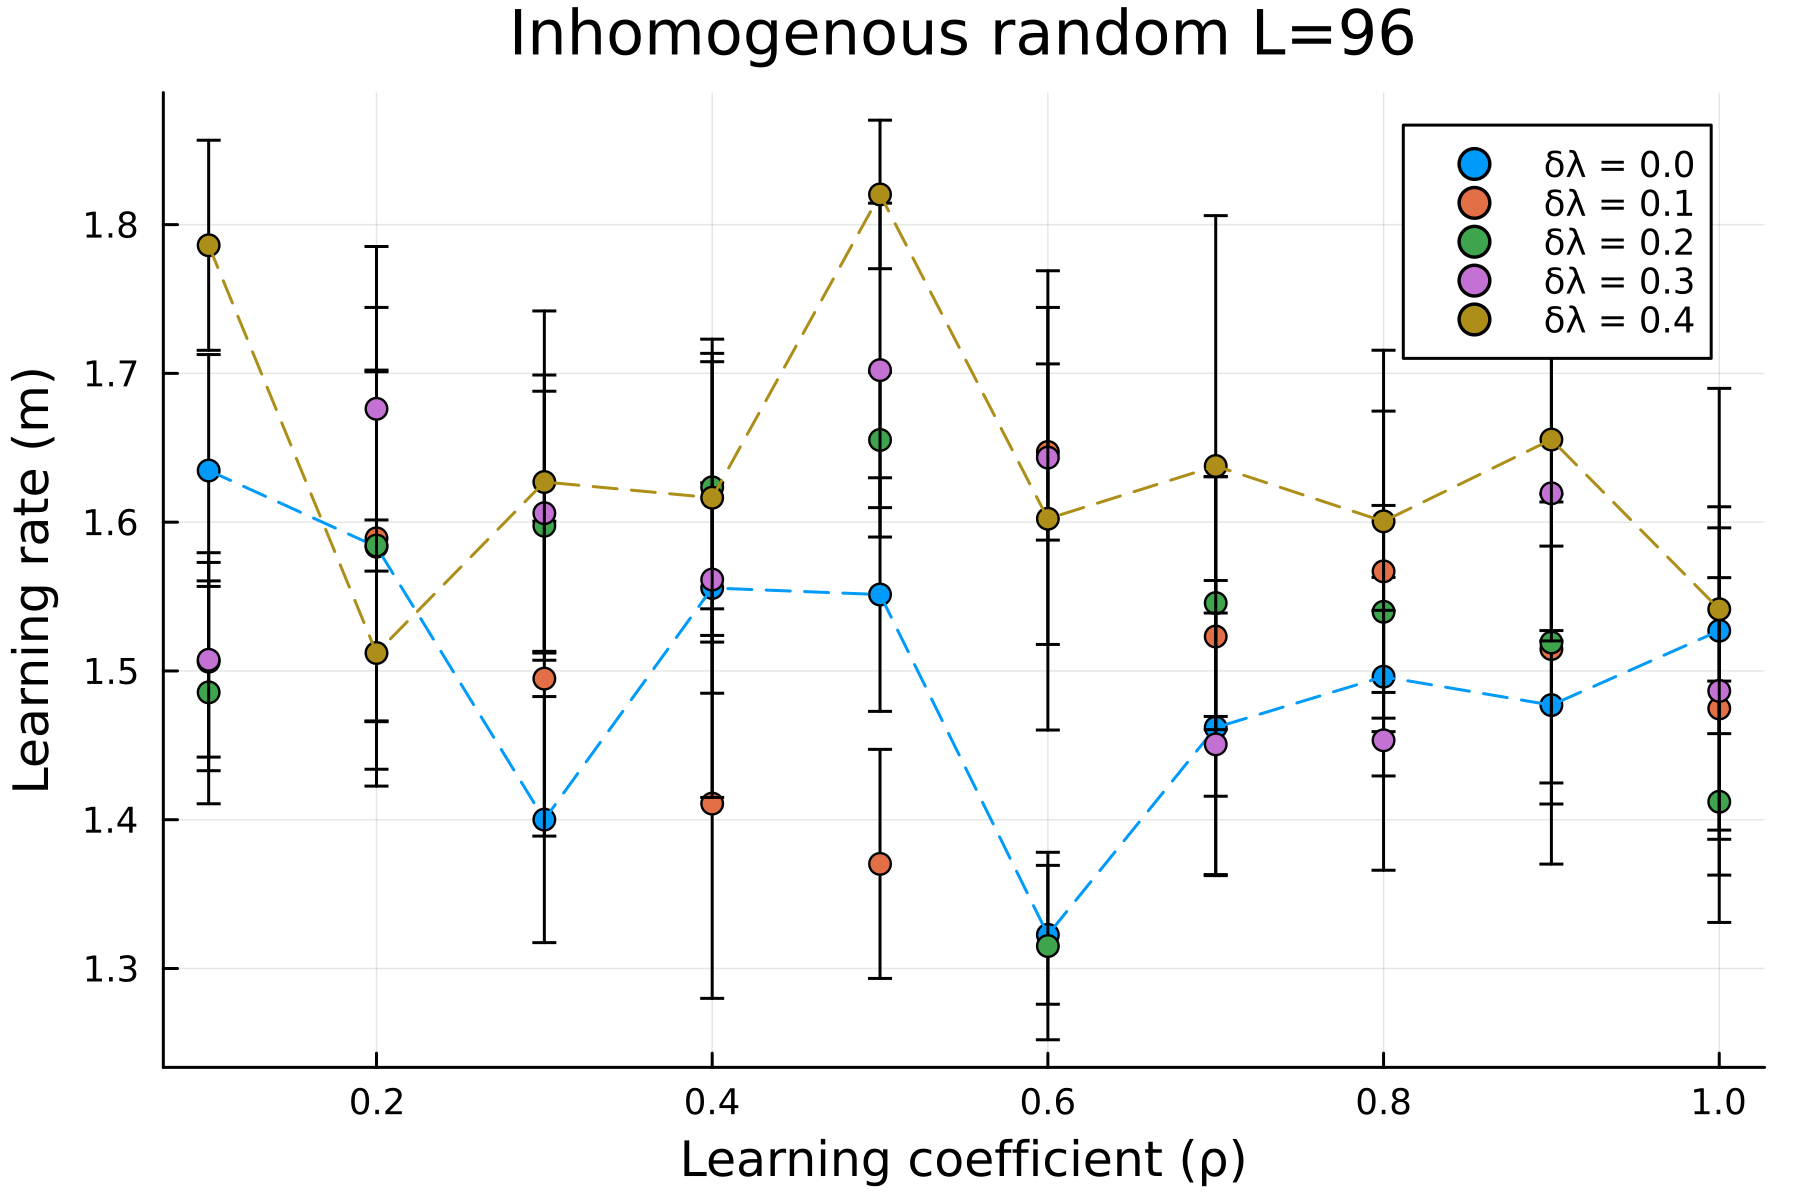
\includegraphics[width=0.40\textwidth]{figures/2D-BPCAIH-analysis/m-plots/m-random-96.png}}
   \subfigure[Traditional $L=128$]{\label{fig:BPCAIH m plot T128}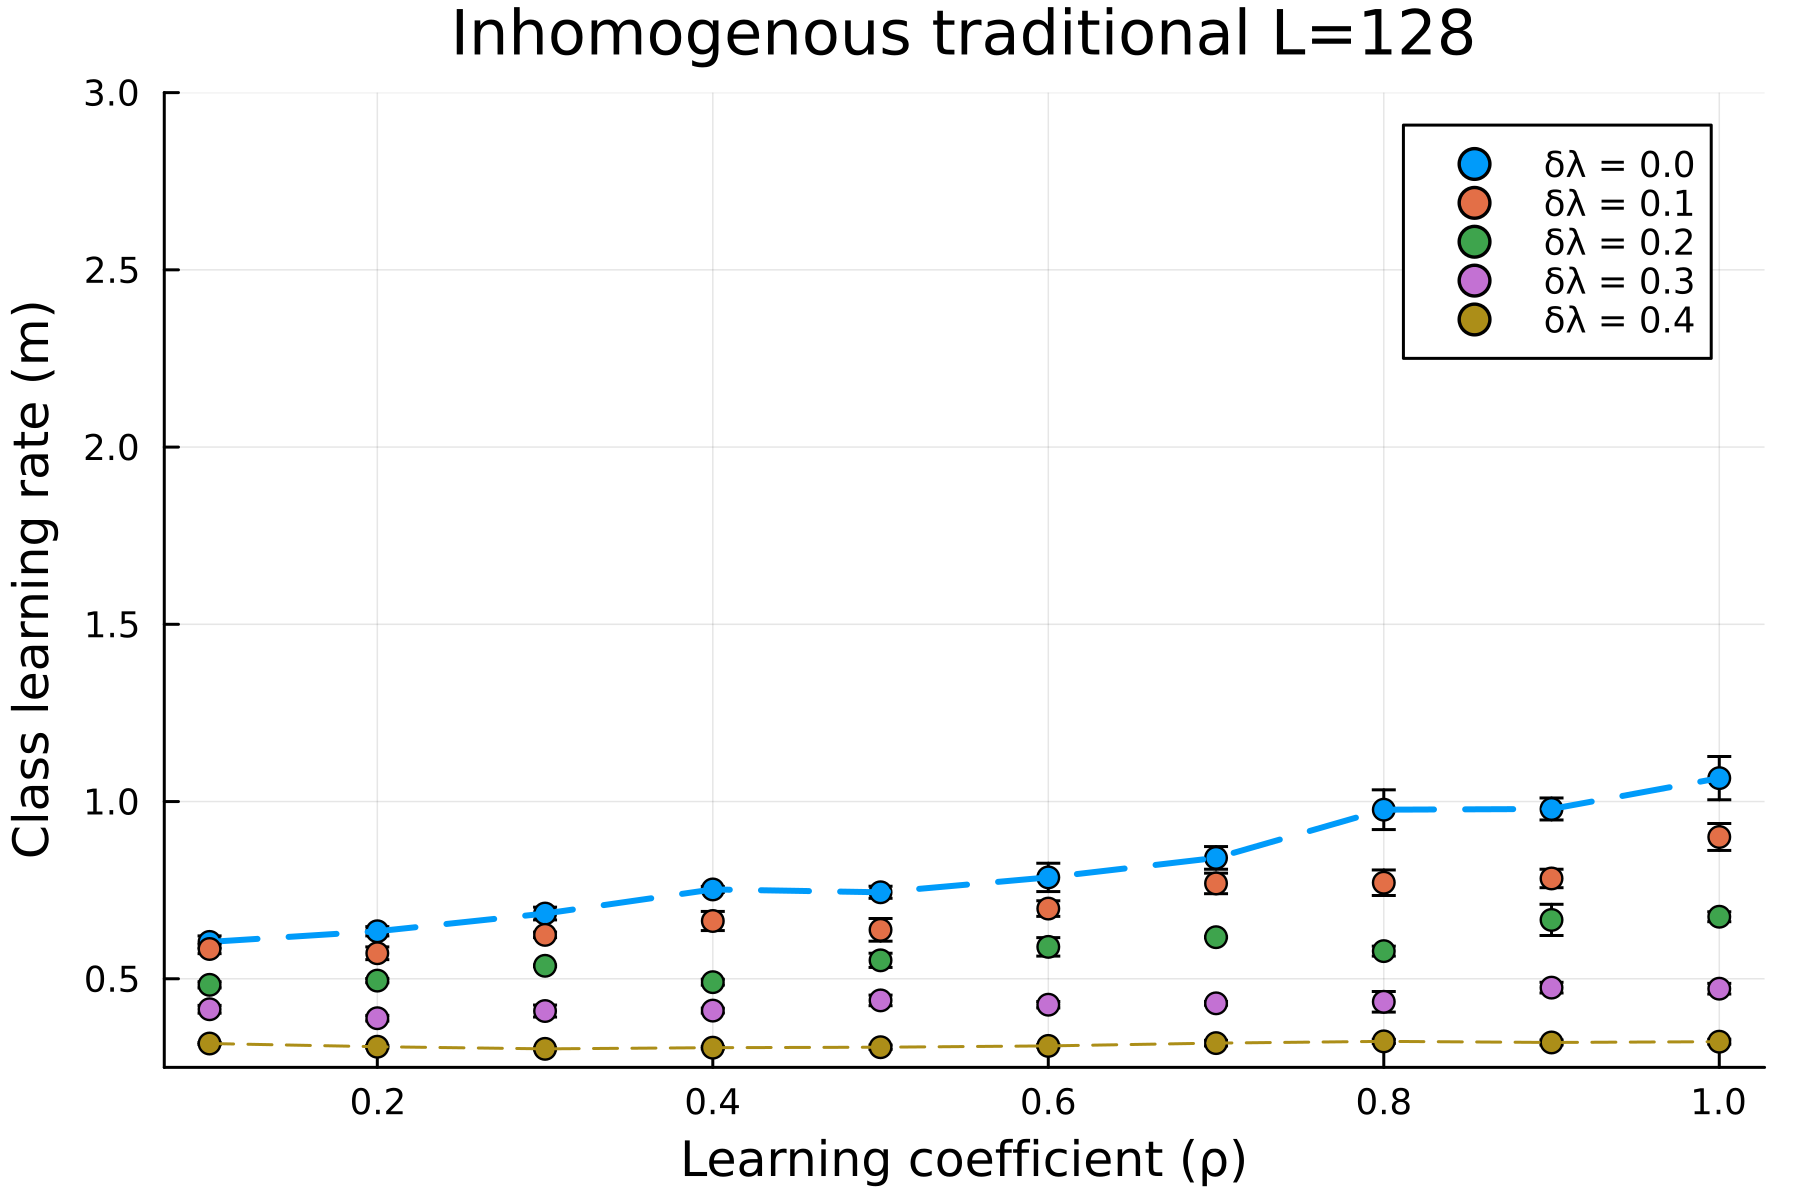
\includegraphics[width=0.40\textwidth]{figures/2D-BPCAIH-analysis/m-plots/m-traditional-128.png}}
   
   \caption[Positional learning factor $\rho_0$ dependence of class learning rate $m$ for the heterogeneous classroom model]{Representative plots for class learning rate $m$ as a function of positional learning coefficient $\rho_0$.
   Each subplot represents a different SA and classroom size $L$.
   In each plot, the circles represent the data points, color represents a different value of $\delta\lambda \in \lbrace 0.0, 0.1, 0.2, 0.3, 0.4 \rbrace$, dashed lines connect the data points for $\delta\lambda \in \lbrace 0.0, 0.4 \rbrace$.
   Higher class learning rate m values indicate better performance.
   }
   \label{fig:2DBPCAIH m rho plot}
\end{figure}

\newpage % new page after section m vs rho

\section{Time to learn $t_{max}$ vs positional learning factor $\rho_0$}\label{sec:BPCAIH t vs rho}
Figure~\ref{fig:2DBPCAIH t-rho plot} shows the time to learn $t_{max}$ is directly affected by the level of heterogeneity $\delta\lambda$. 
This means that the heterogeneity $\delta\lambda$ has a significant effect on the time to learn $t_{max}$, with lower values of $\delta\lambda$ leading to lower time to learn $t_{max}$ for all values of $\rho_0$. 
We also notice that the traditional model is more affected by classroom heterogeneity compared to PI models.

When aggregating the different results for each class size $L$, as shown in Figure~\ref{fig:2DBPCAIH t-rho ribbon plot}, it affirms our previous findings that PI models are better for smaller classes and lower values of $\rho_0$.
This stays consistent when comparing the performance of a similar classroom size $L$ and heterogeneity $\delta\lambda$ using the traditional model.
However, the comparison is not as clear when comparing between different levels of heterogeneity $\delta\lambda$.
When $L\geq64$, the PI models can perform better than the traditional model depending on the heterogeneity $\delta\lambda$, even with the same positional learning factor $\rho_0$.

\begin{figure}[htbp!]
   \centering
   \subfigure[Outer corner $L=48$]{\label{fig:2DBPCAIH t-rho plot OC48}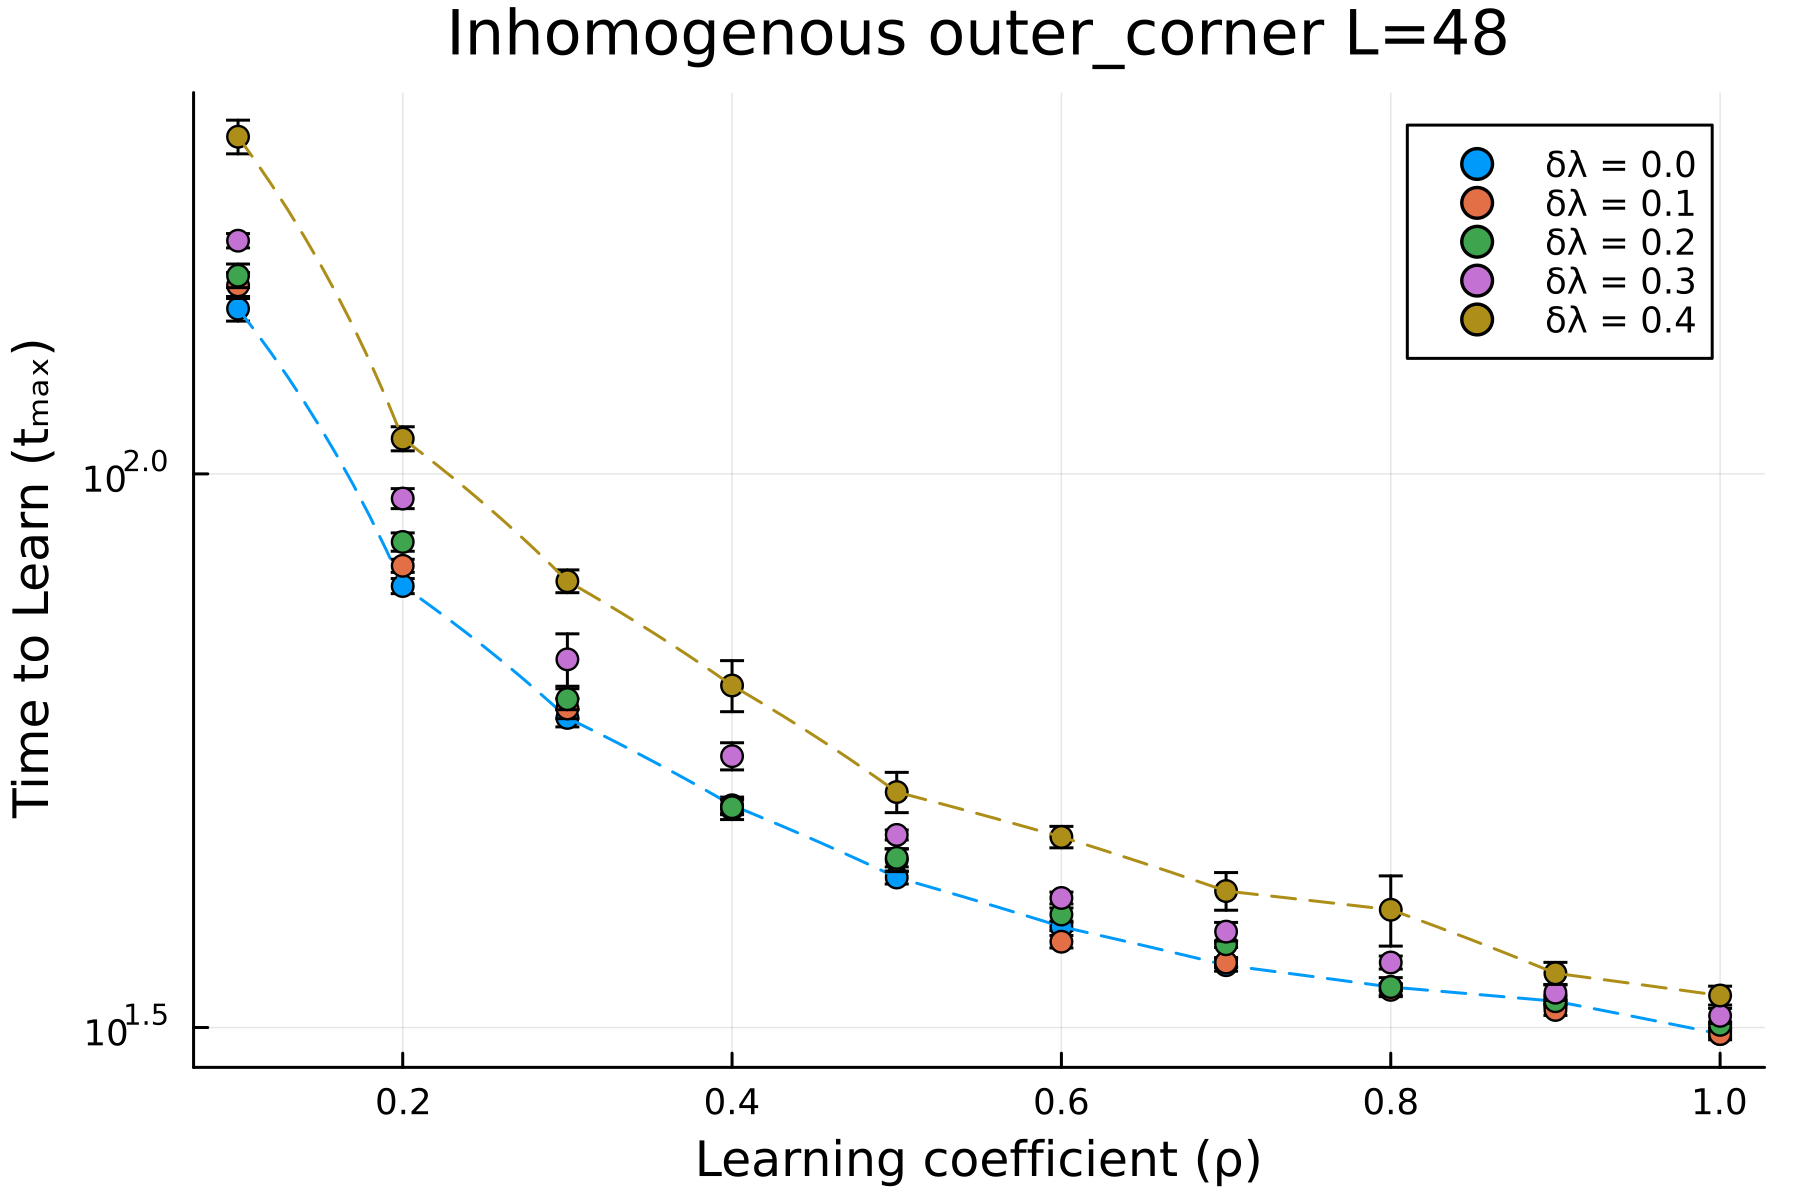
\includegraphics[width=0.49\textwidth]{figures/2D-BPCAIH-analysis/t-plots/t-outer_corner-48.png}}
   \subfigure[Outer corner $L=96$]{\label{fig:2DBPCAIH t-rho plot OC96}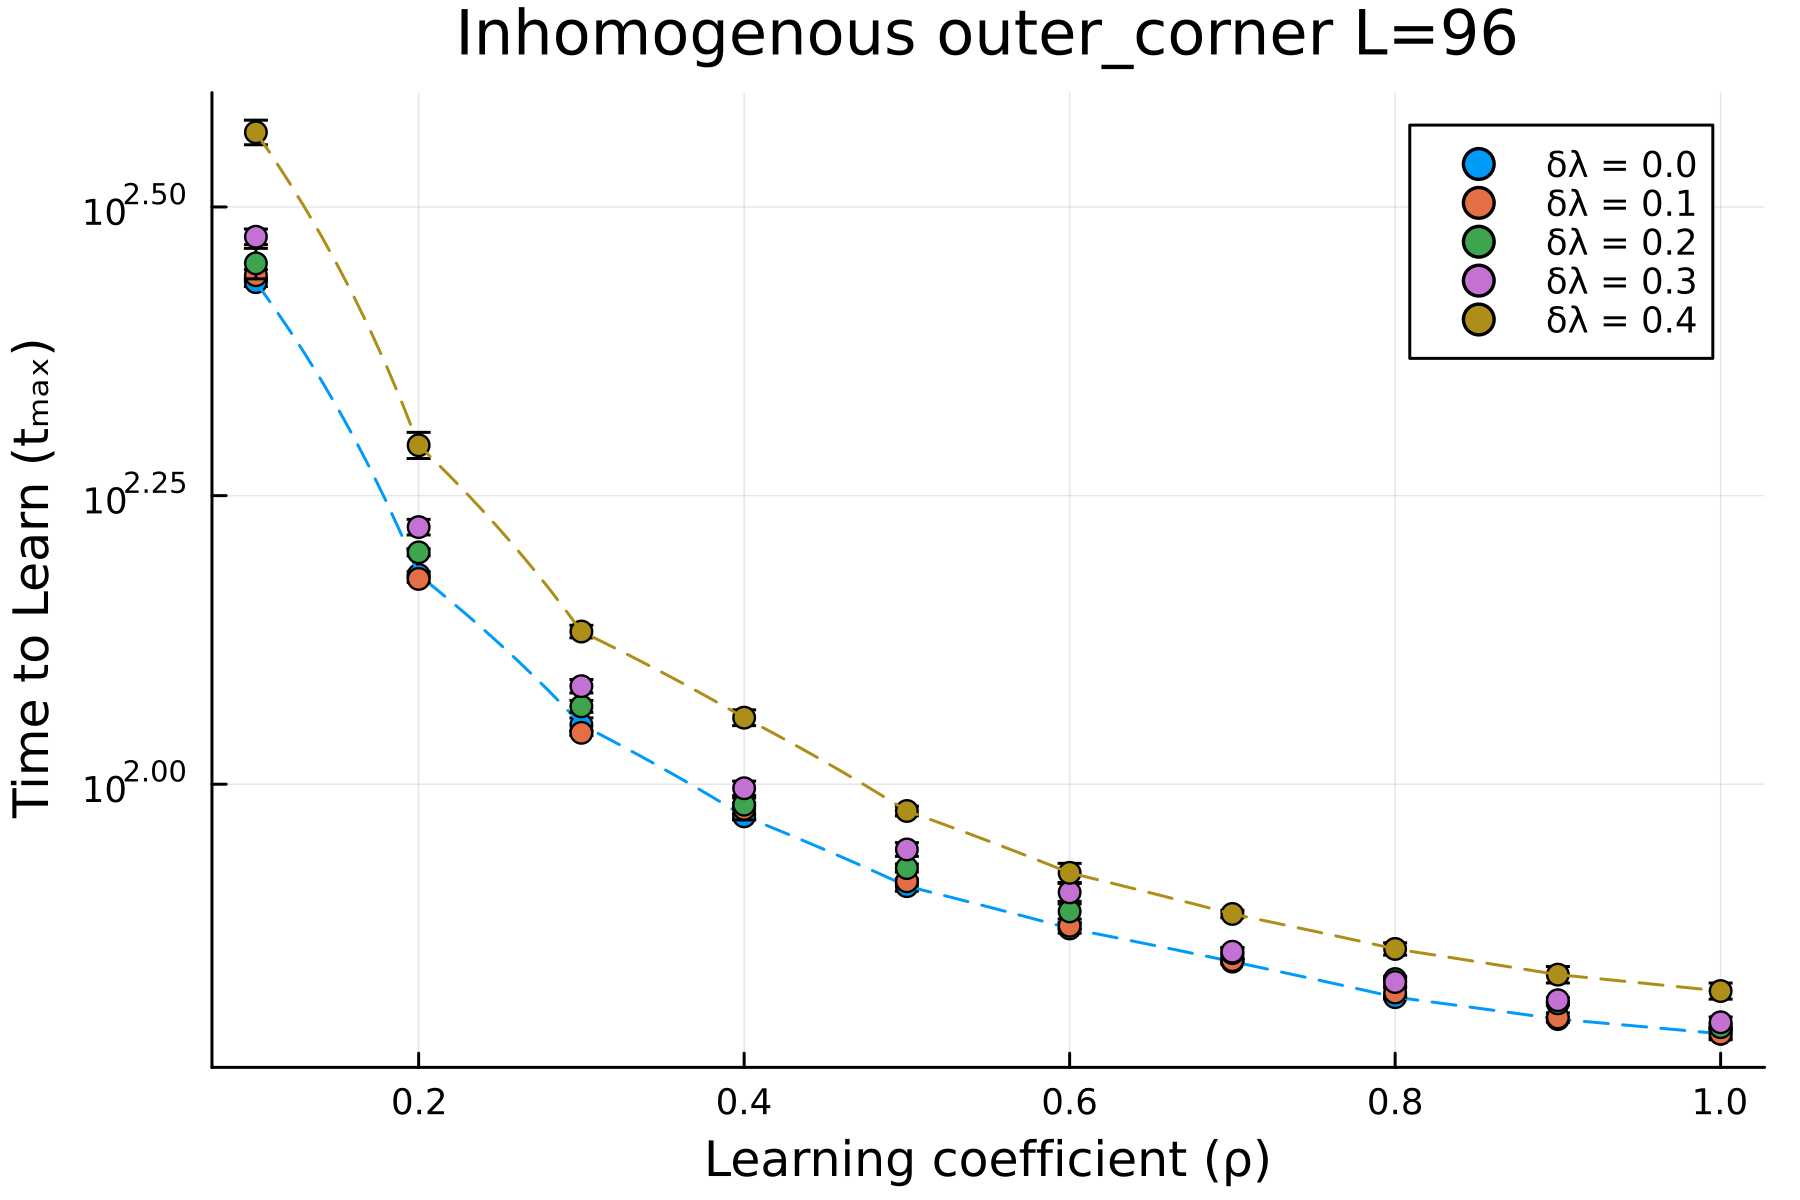
\includegraphics[width=0.49\textwidth]{figures/2D-BPCAIH-analysis/t-plots/t-outer_corner-96.png}}
   \subfigure[Inner corner $L=48$]{\label{fig:2DBPCAIH t-rho plot IC48}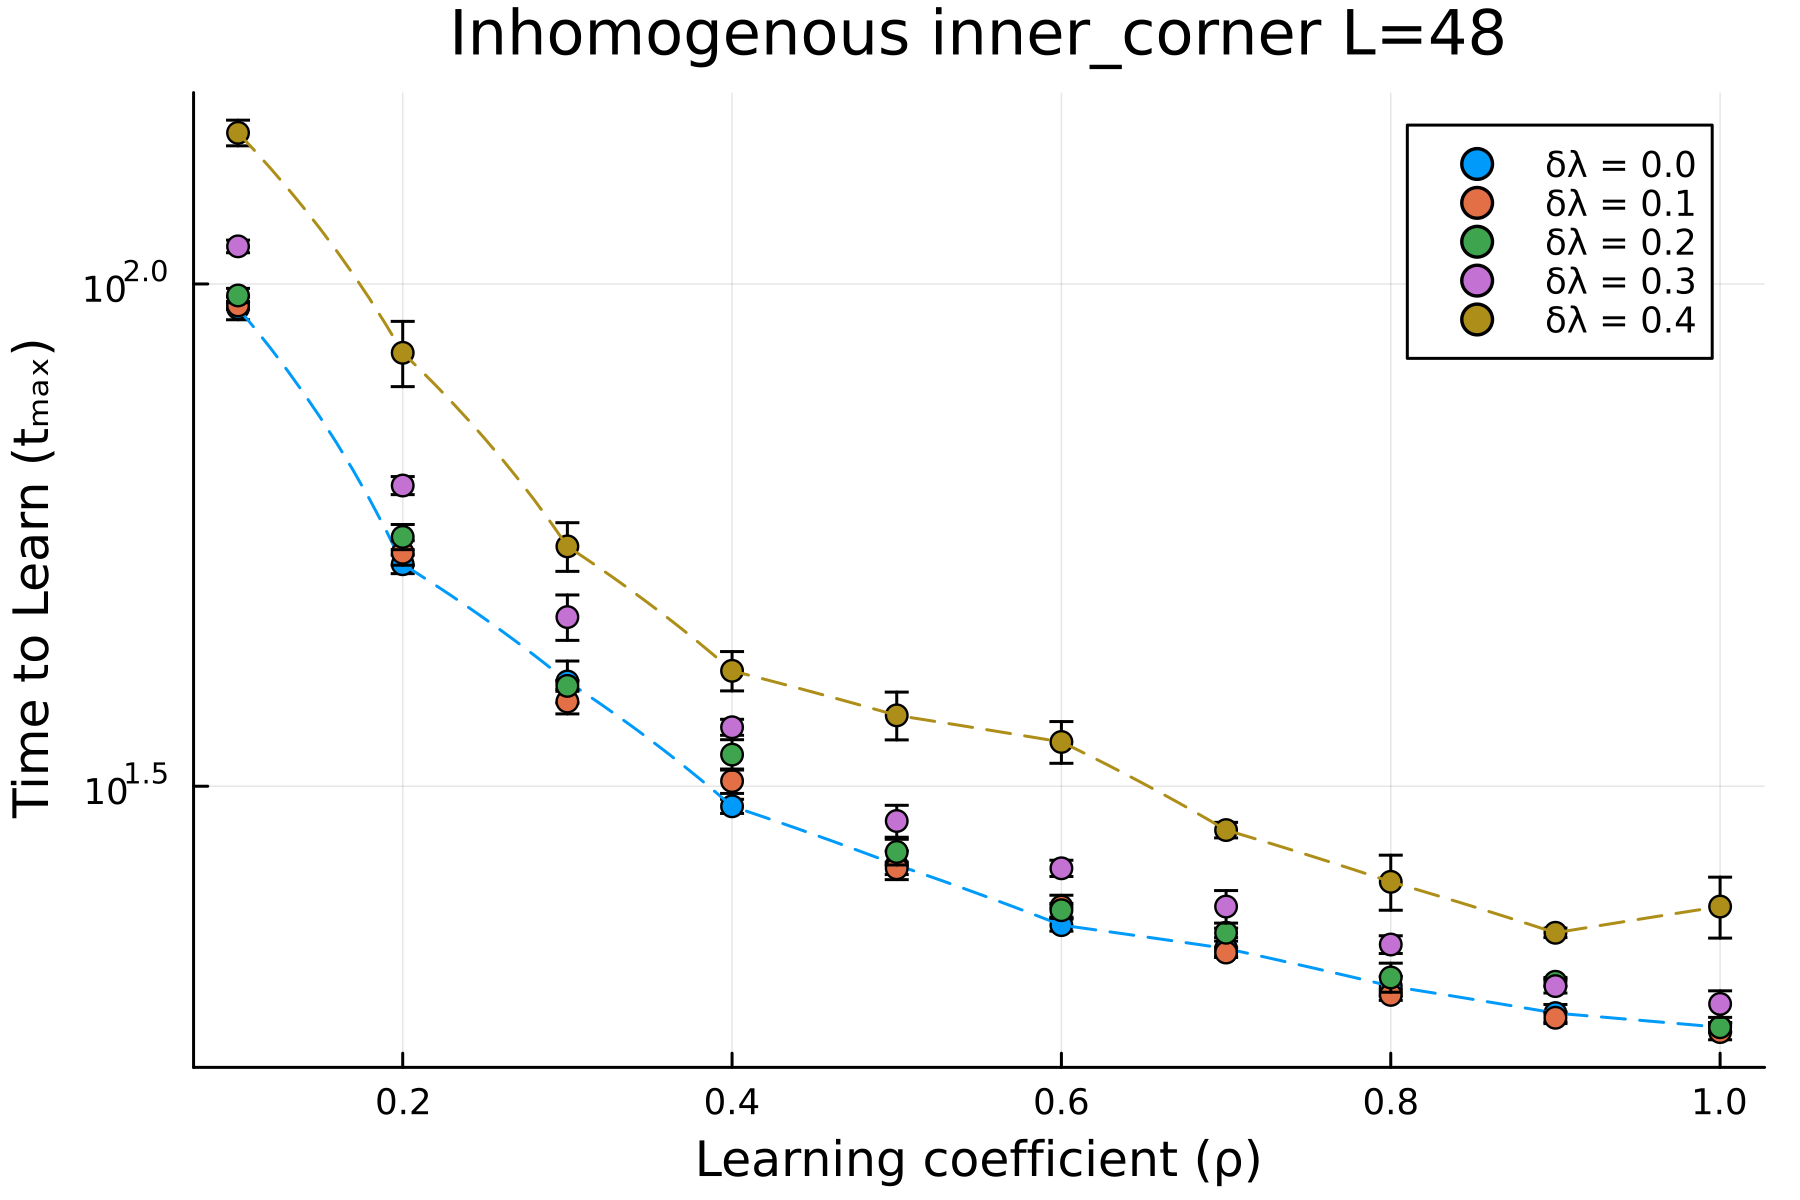
\includegraphics[width=0.49\textwidth]{figures/2D-BPCAIH-analysis/t-plots/t-inner_corner-48.png}}
   \subfigure[Inner corner $L=96$]{\label{fig:2DBPCAIH t-rho plot IC96}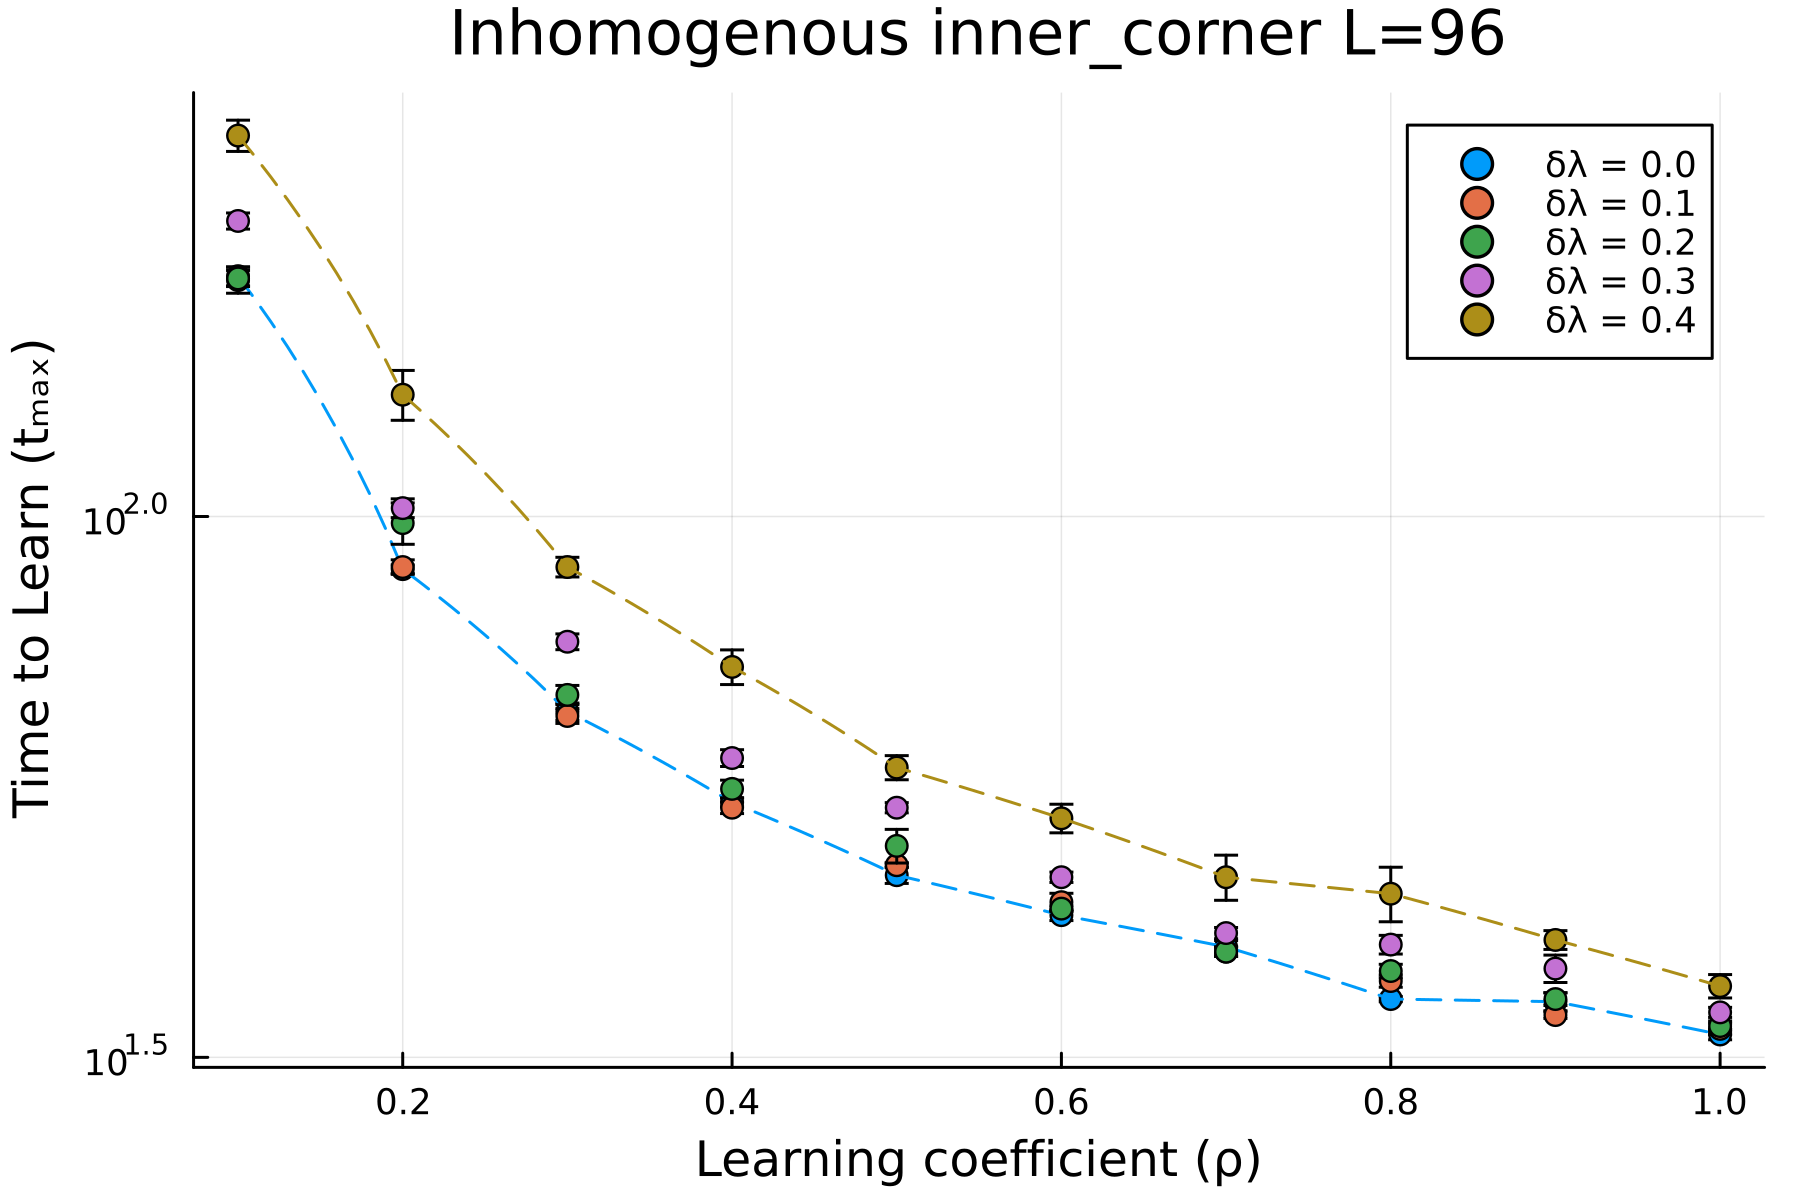
\includegraphics[width=0.49\textwidth]{figures/2D-BPCAIH-analysis/t-plots/t-inner_corner-96.png}}
   \subfigure[Traditional $L=48$]{\label{fig:2DBPCAIH t-rho plot T48}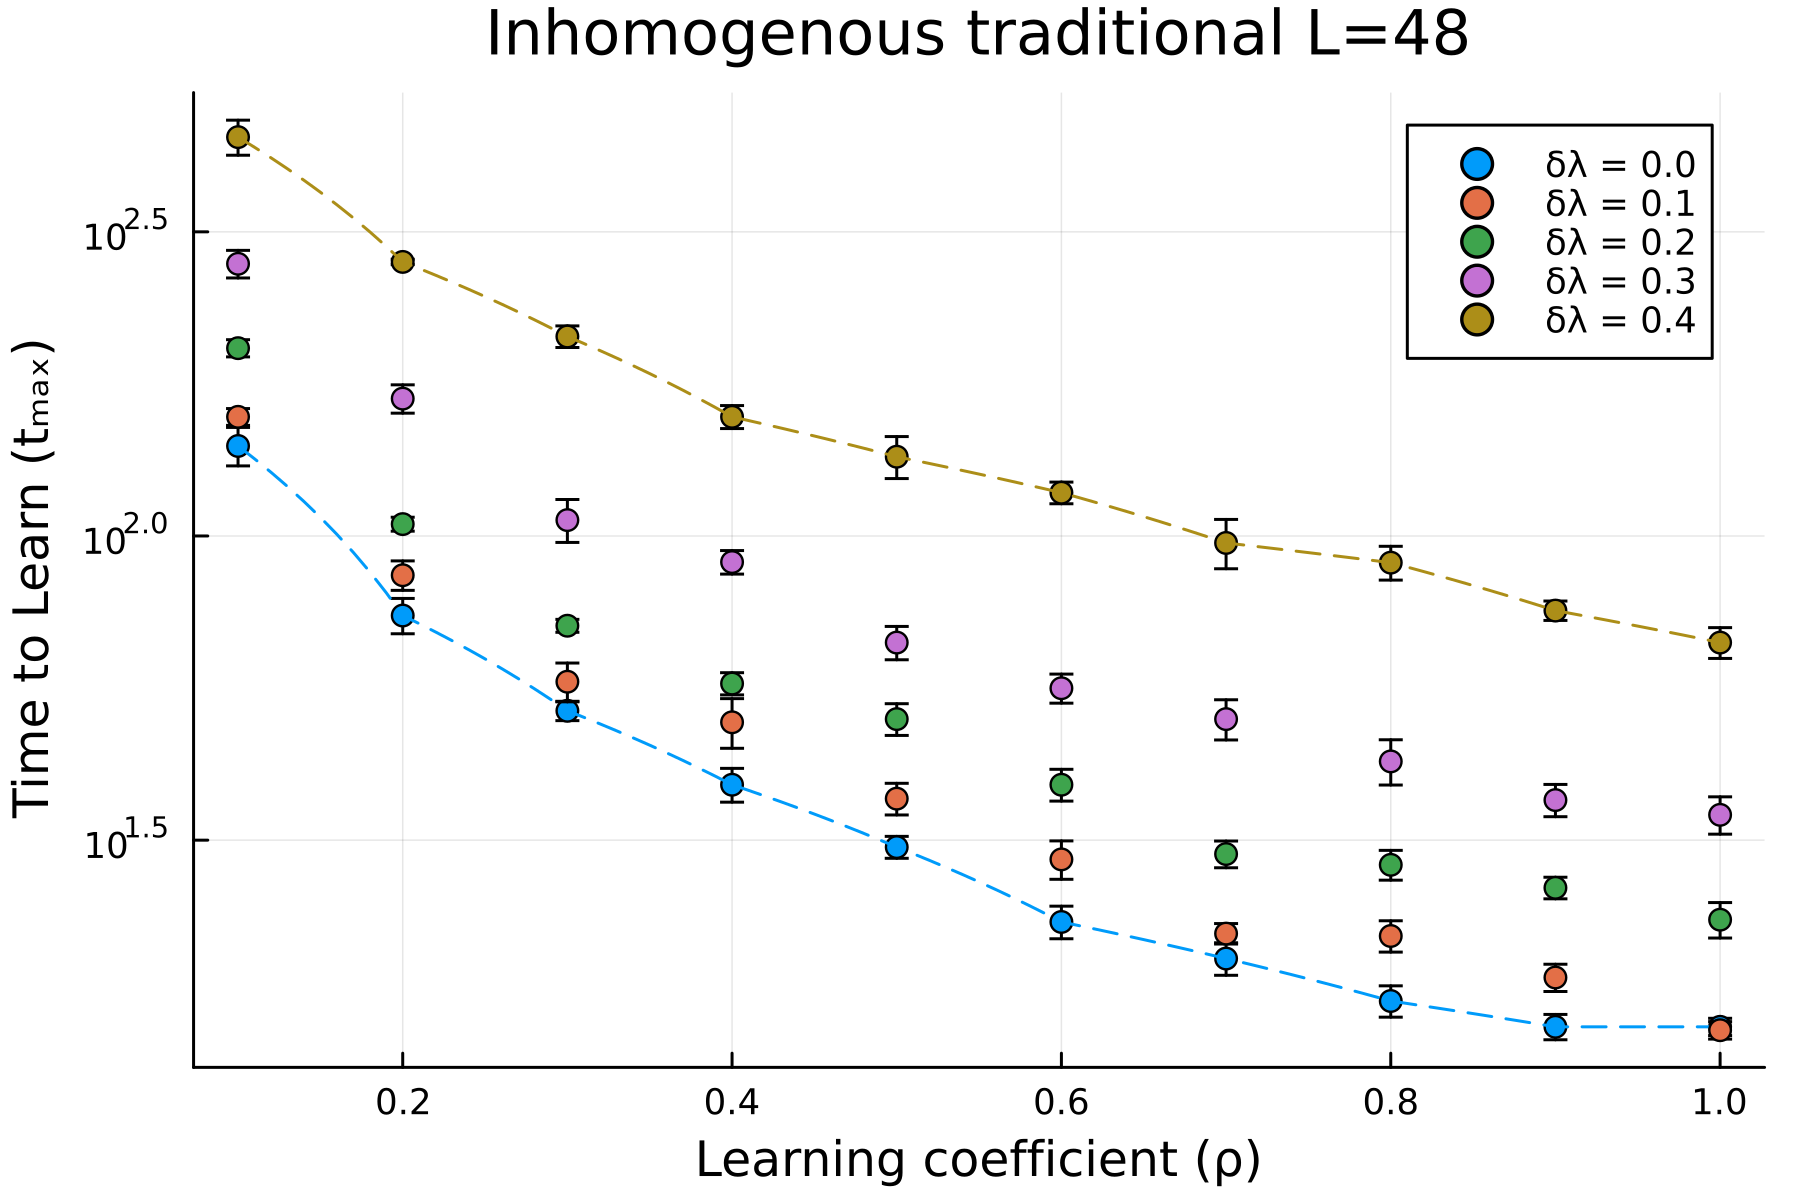
\includegraphics[width=0.49\textwidth]{figures/2D-BPCAIH-analysis/t-plots/t-traditional-48.png}}
   \subfigure[Traditional $L=96$]{\label{fig:2DBPCAIH t-rho plot T96}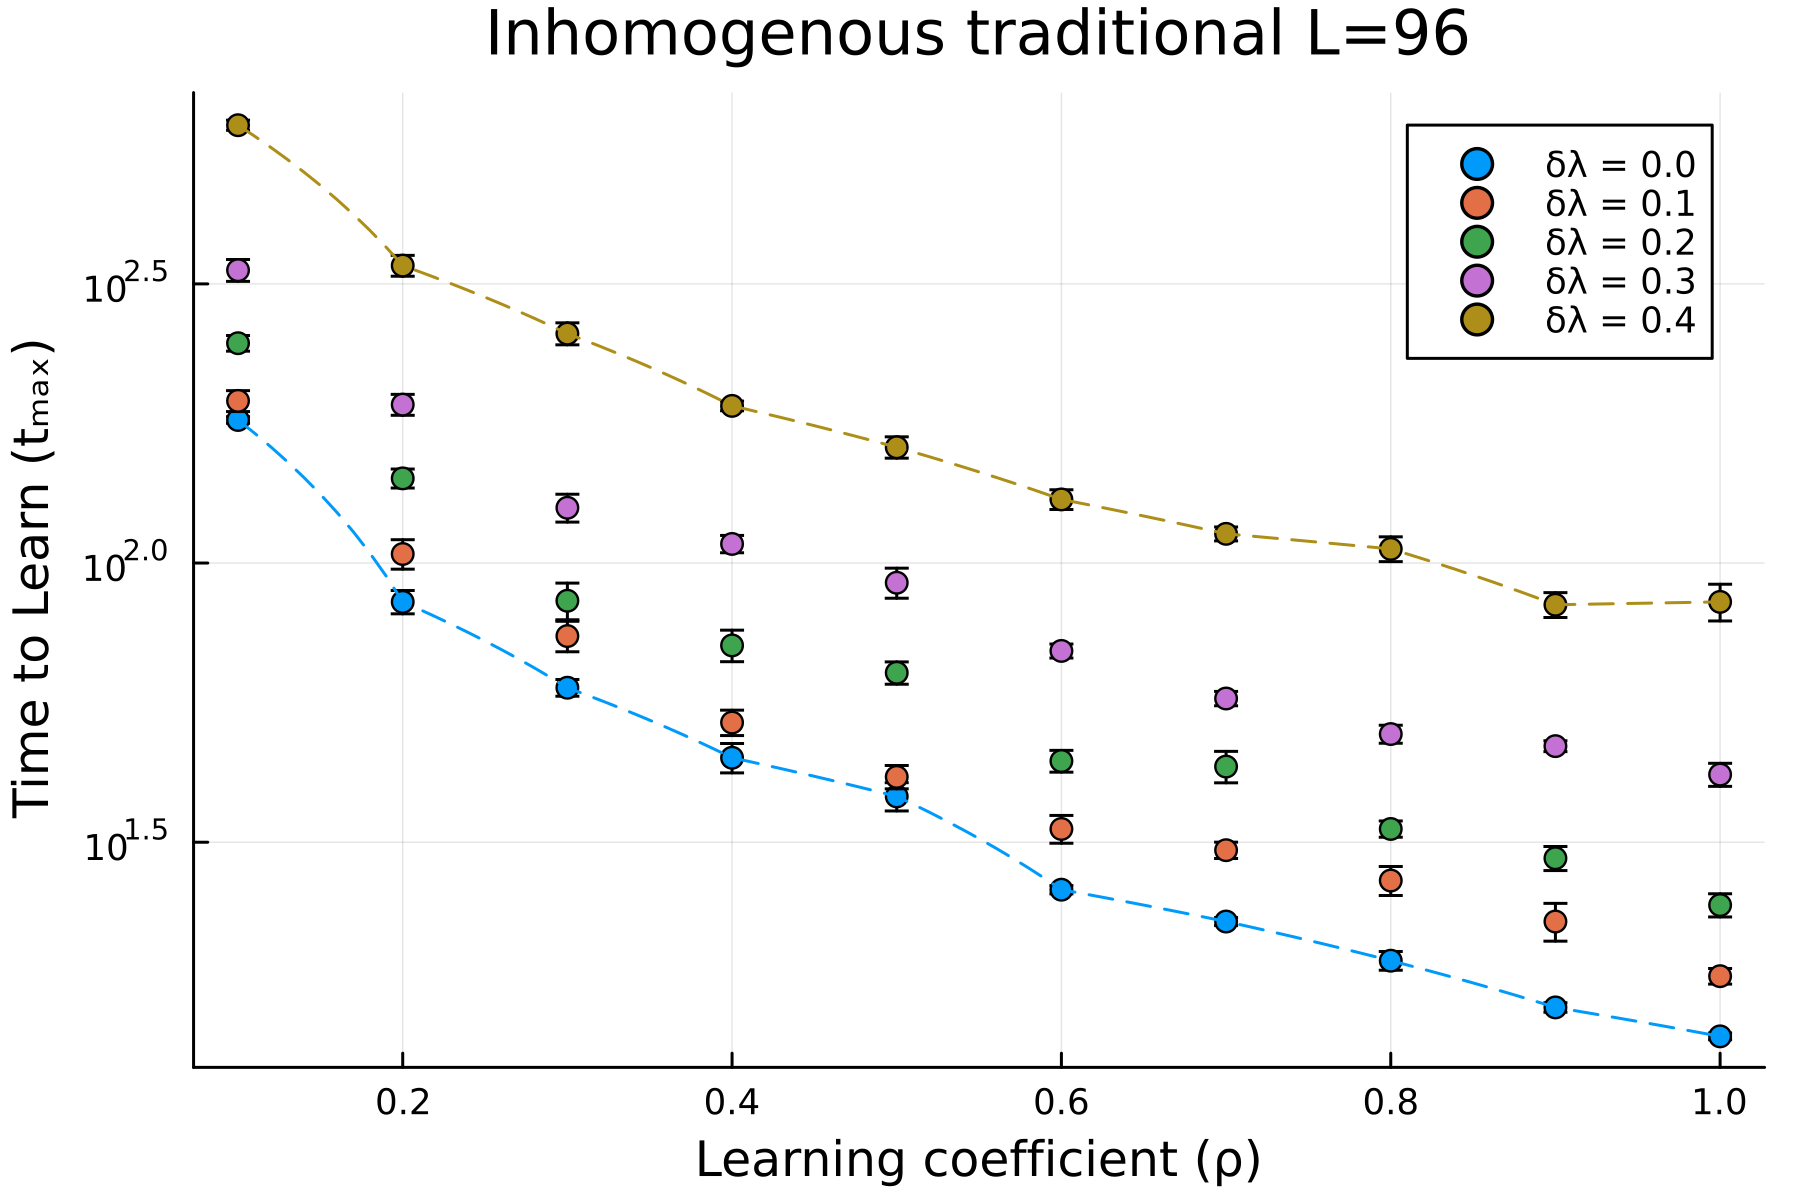
\includegraphics[width=0.49\textwidth]{figures/2D-BPCAIH-analysis/t-plots/t-traditional-96.png}}
   \caption[Positional learning factor $\rho_0$ dependence of time to learn $t_{max}$ for the heterogeneous classroom model for representative SAs and heterogeneity $\delta\lambda$]{Time to learn $t_{max}$ as a function of positional learning factor $\rho_0$ for different representative classroom configurations and sizes with varying heterogeneity $\delta\lambda \in \lbrace 0, 0.1, 0.2, 0.3, 0.4 \rbrace$. Lower time to learn $t_{max}$ indicates better performance.}
   \label{fig:2DBPCAIH t-rho plot}
\end{figure}


\begin{figure}[htbp!]
   \centering
   \subfigure[$L=32$]{\label{fig:2DBPCAIH t-rho ribbon plot 32}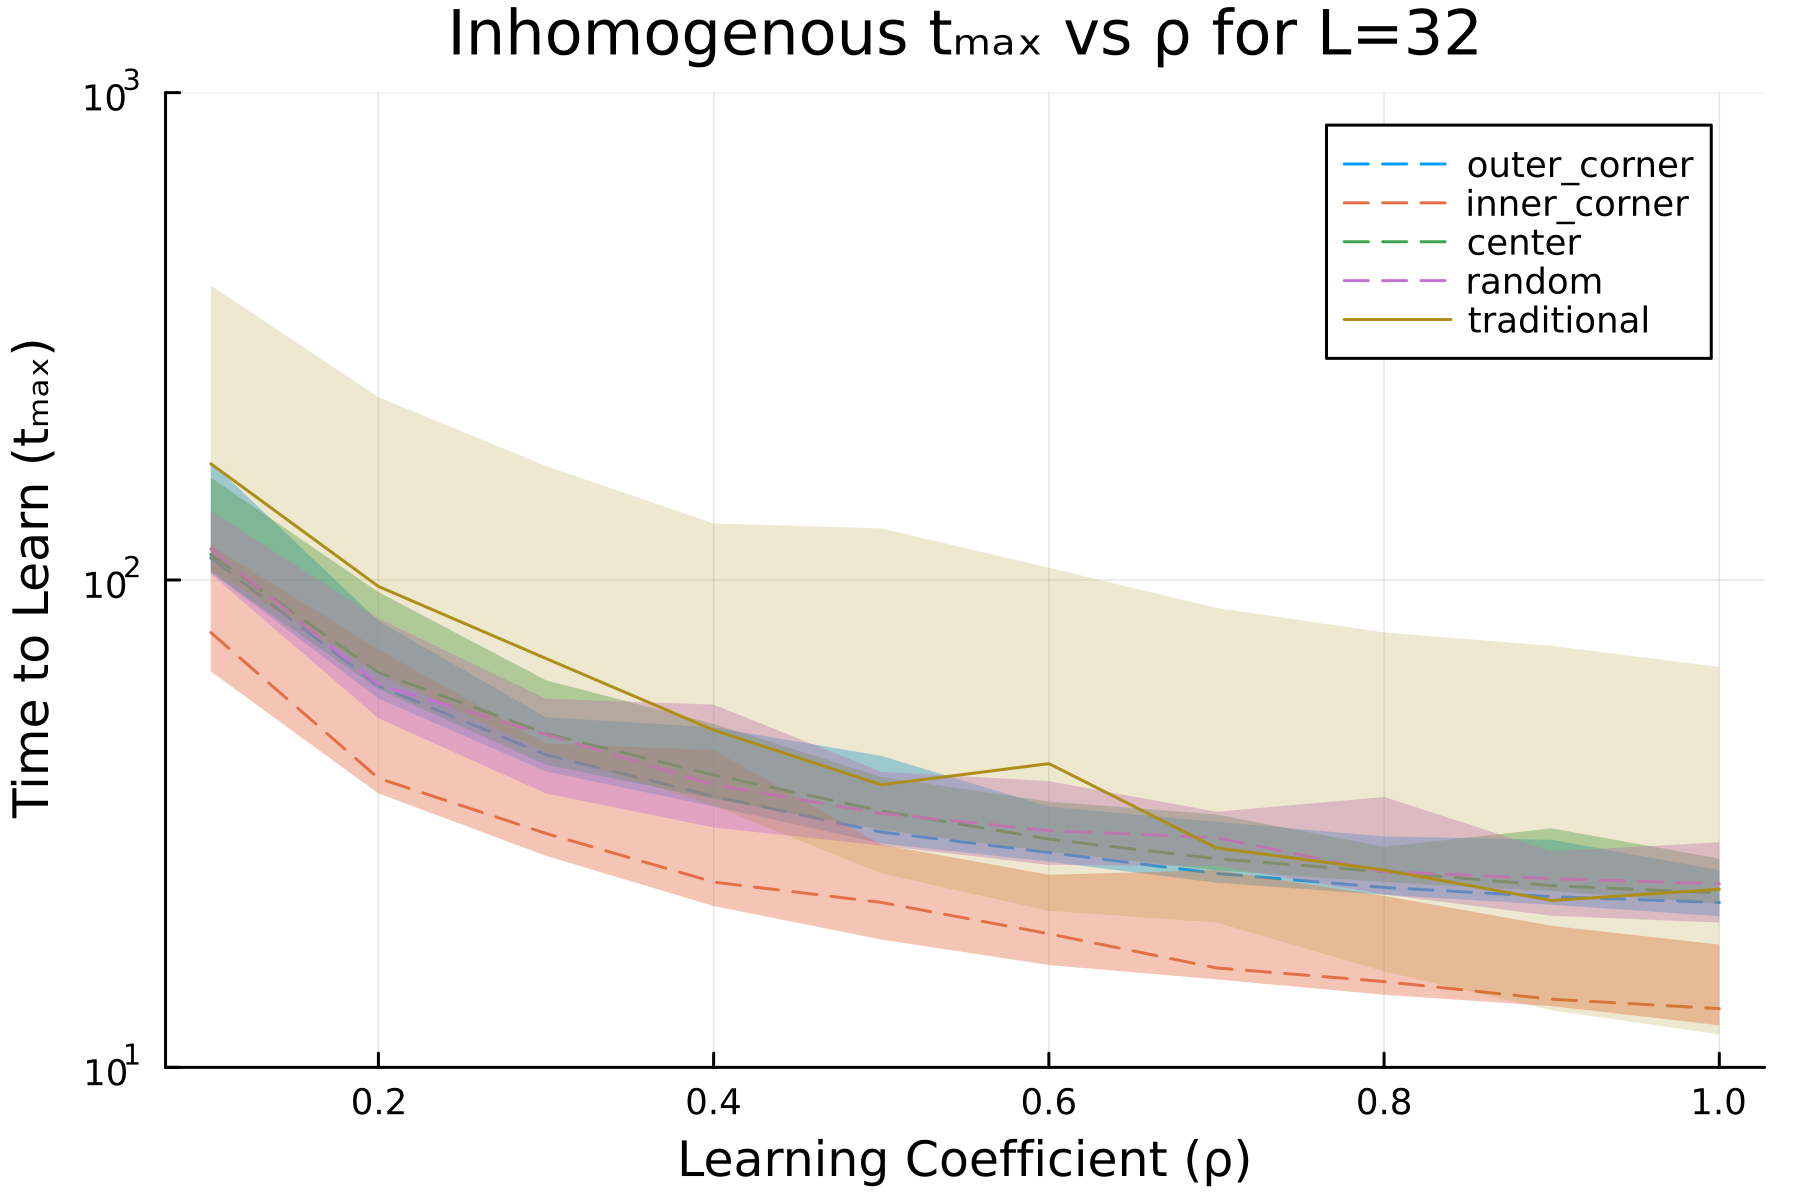
\includegraphics[width=0.49\textwidth]{figures/2D-BPCAIH-analysis/rho-t ribbon plots/rho-t-ribbon-32.png}}
   \subfigure[$L=48$]{\label{fig:2DBPCAIH t-rho ribbon plot 48}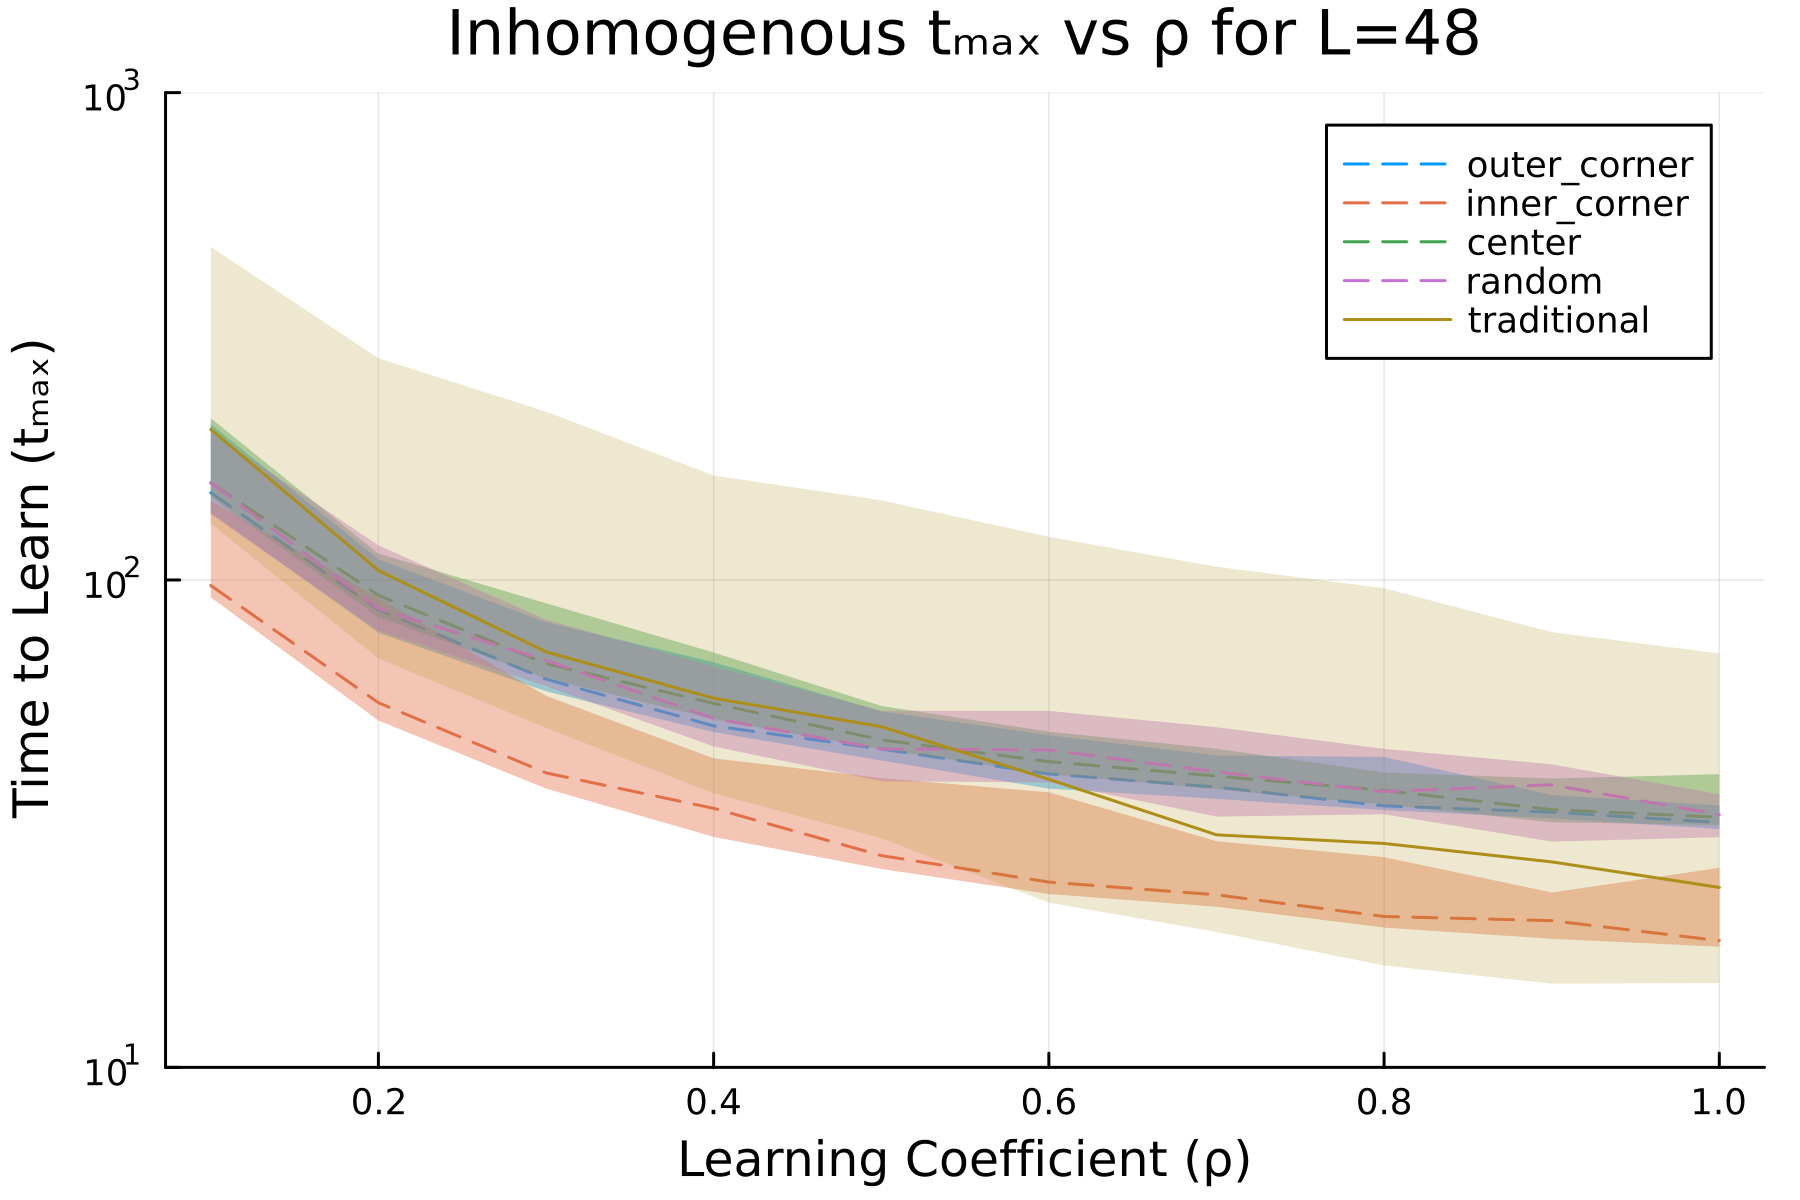
\includegraphics[width=0.49\textwidth]{figures/2D-BPCAIH-analysis/rho-t ribbon plots/rho-t-ribbon-48.png}}
   \subfigure[$L=64$]{\label{fig:2DBPCAIH t-rho ribbon plot 64}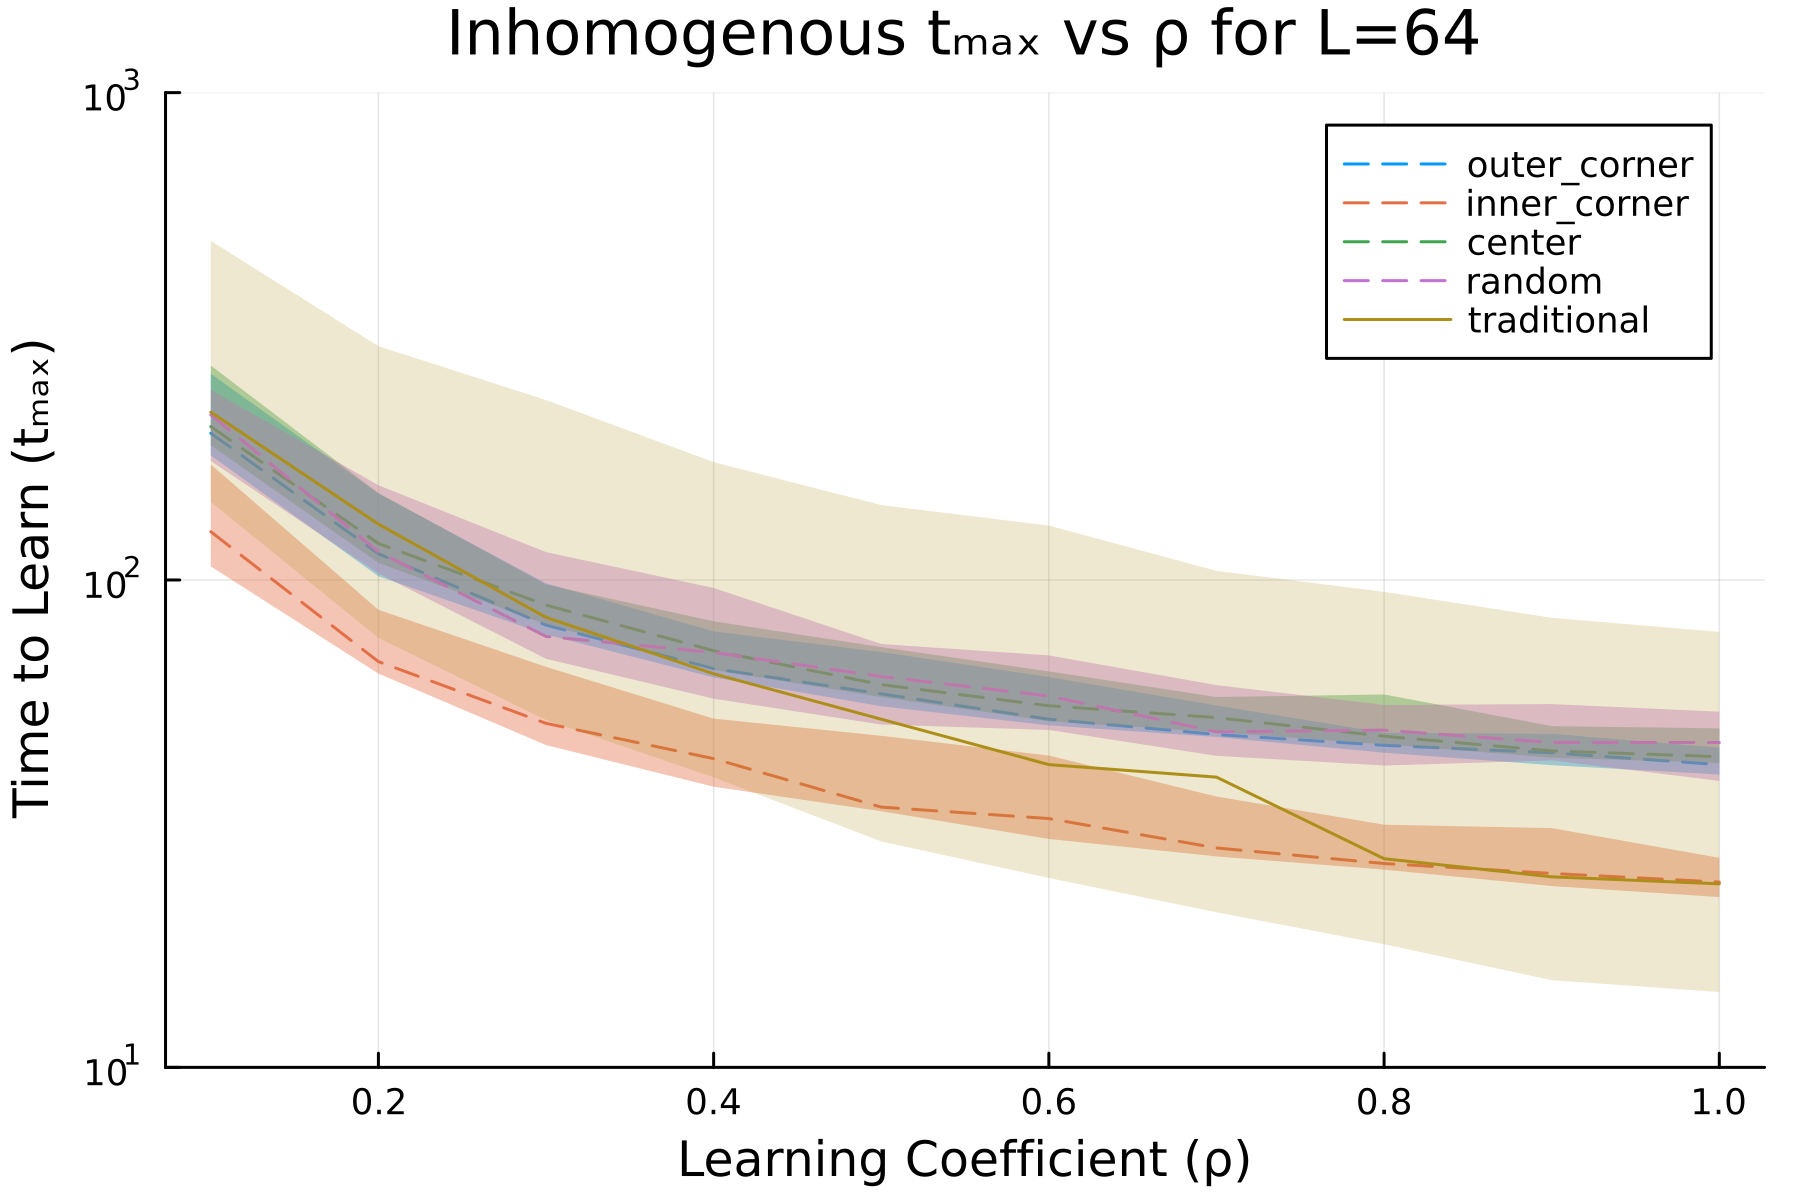
\includegraphics[width=0.49\textwidth]{figures/2D-BPCAIH-analysis/rho-t ribbon plots/rho-t-ribbon-64.png}}
   \subfigure[$L=96$]{\label{fig:2DBPCAIH t-rho ribbon plot 96}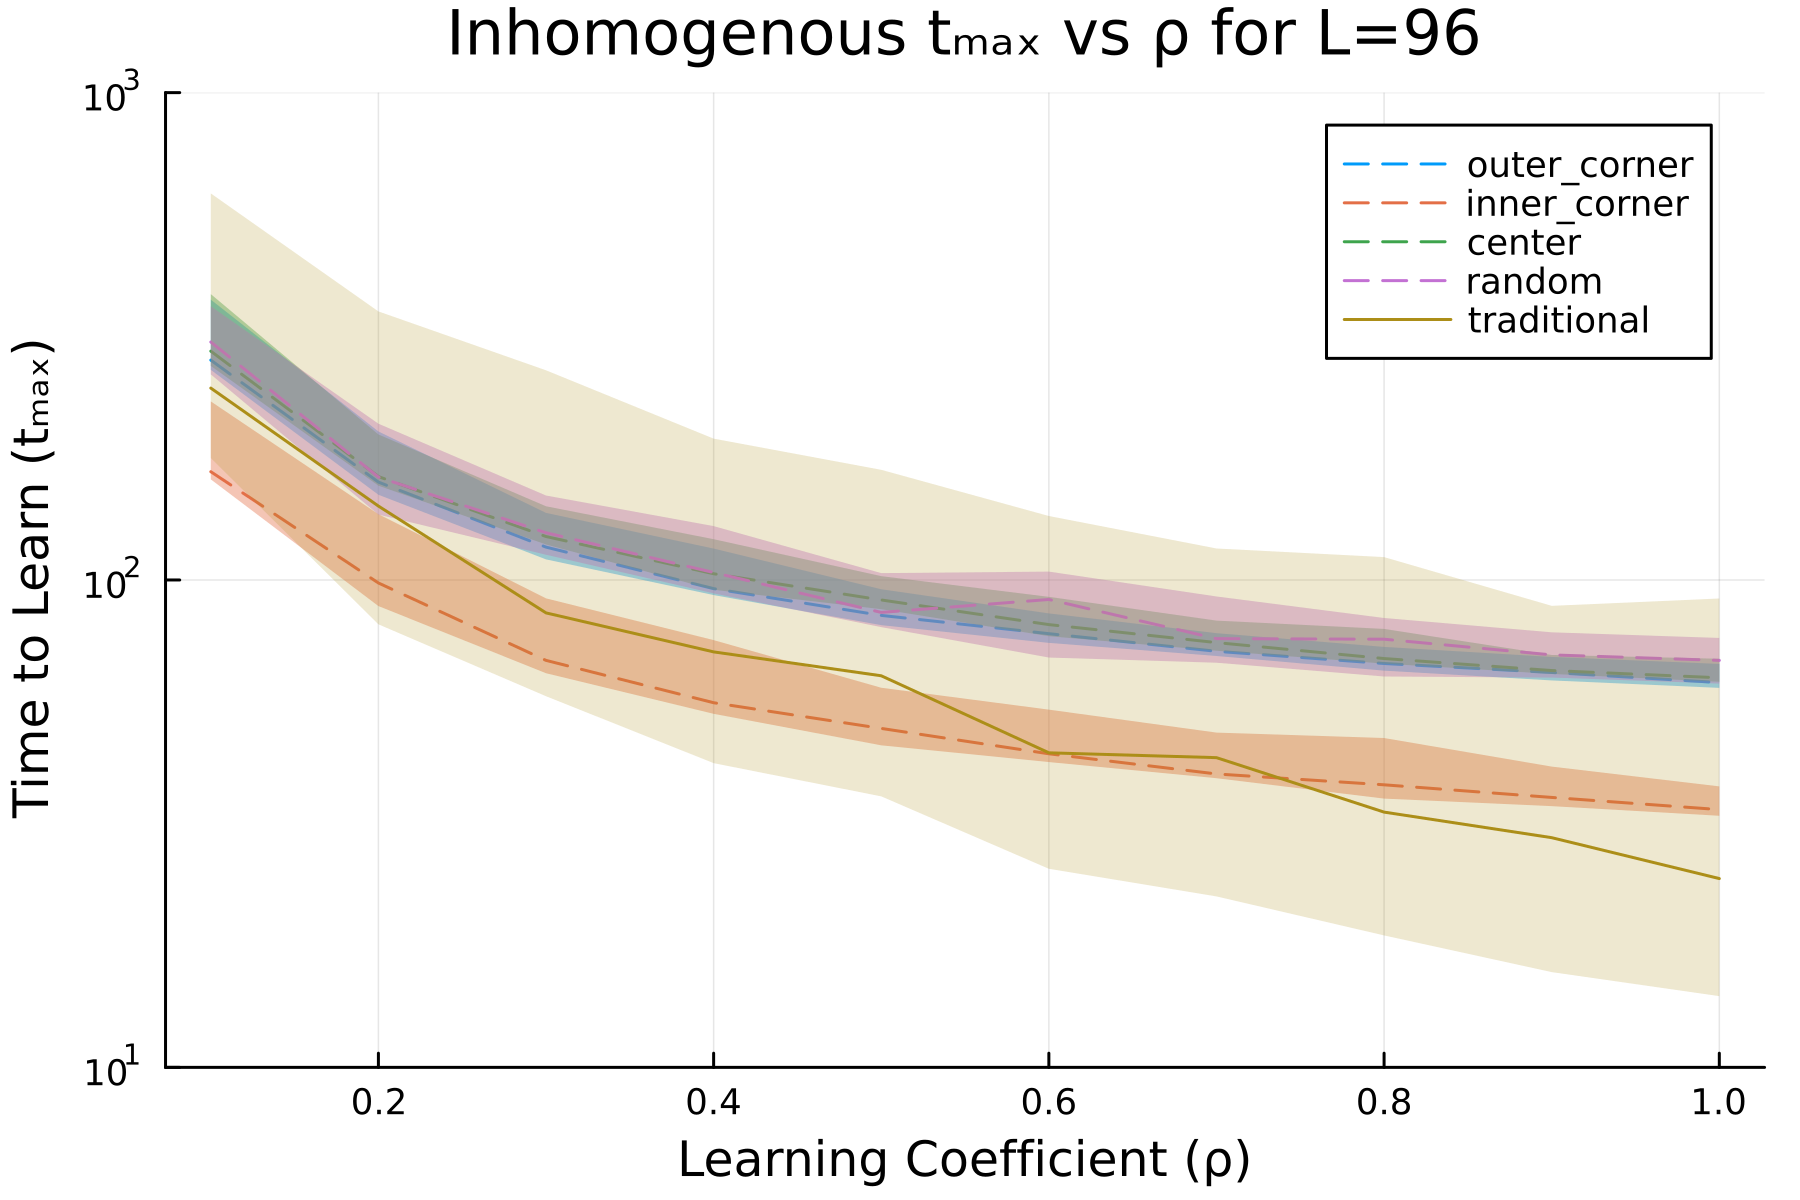
\includegraphics[width=0.49\textwidth]{figures/2D-BPCAIH-analysis/rho-t ribbon plots/rho-t-ribbon-96.png}}
   \subfigure[$L=128$]{\label{fig:2DBPCAIH t-rho ribbon plot 128}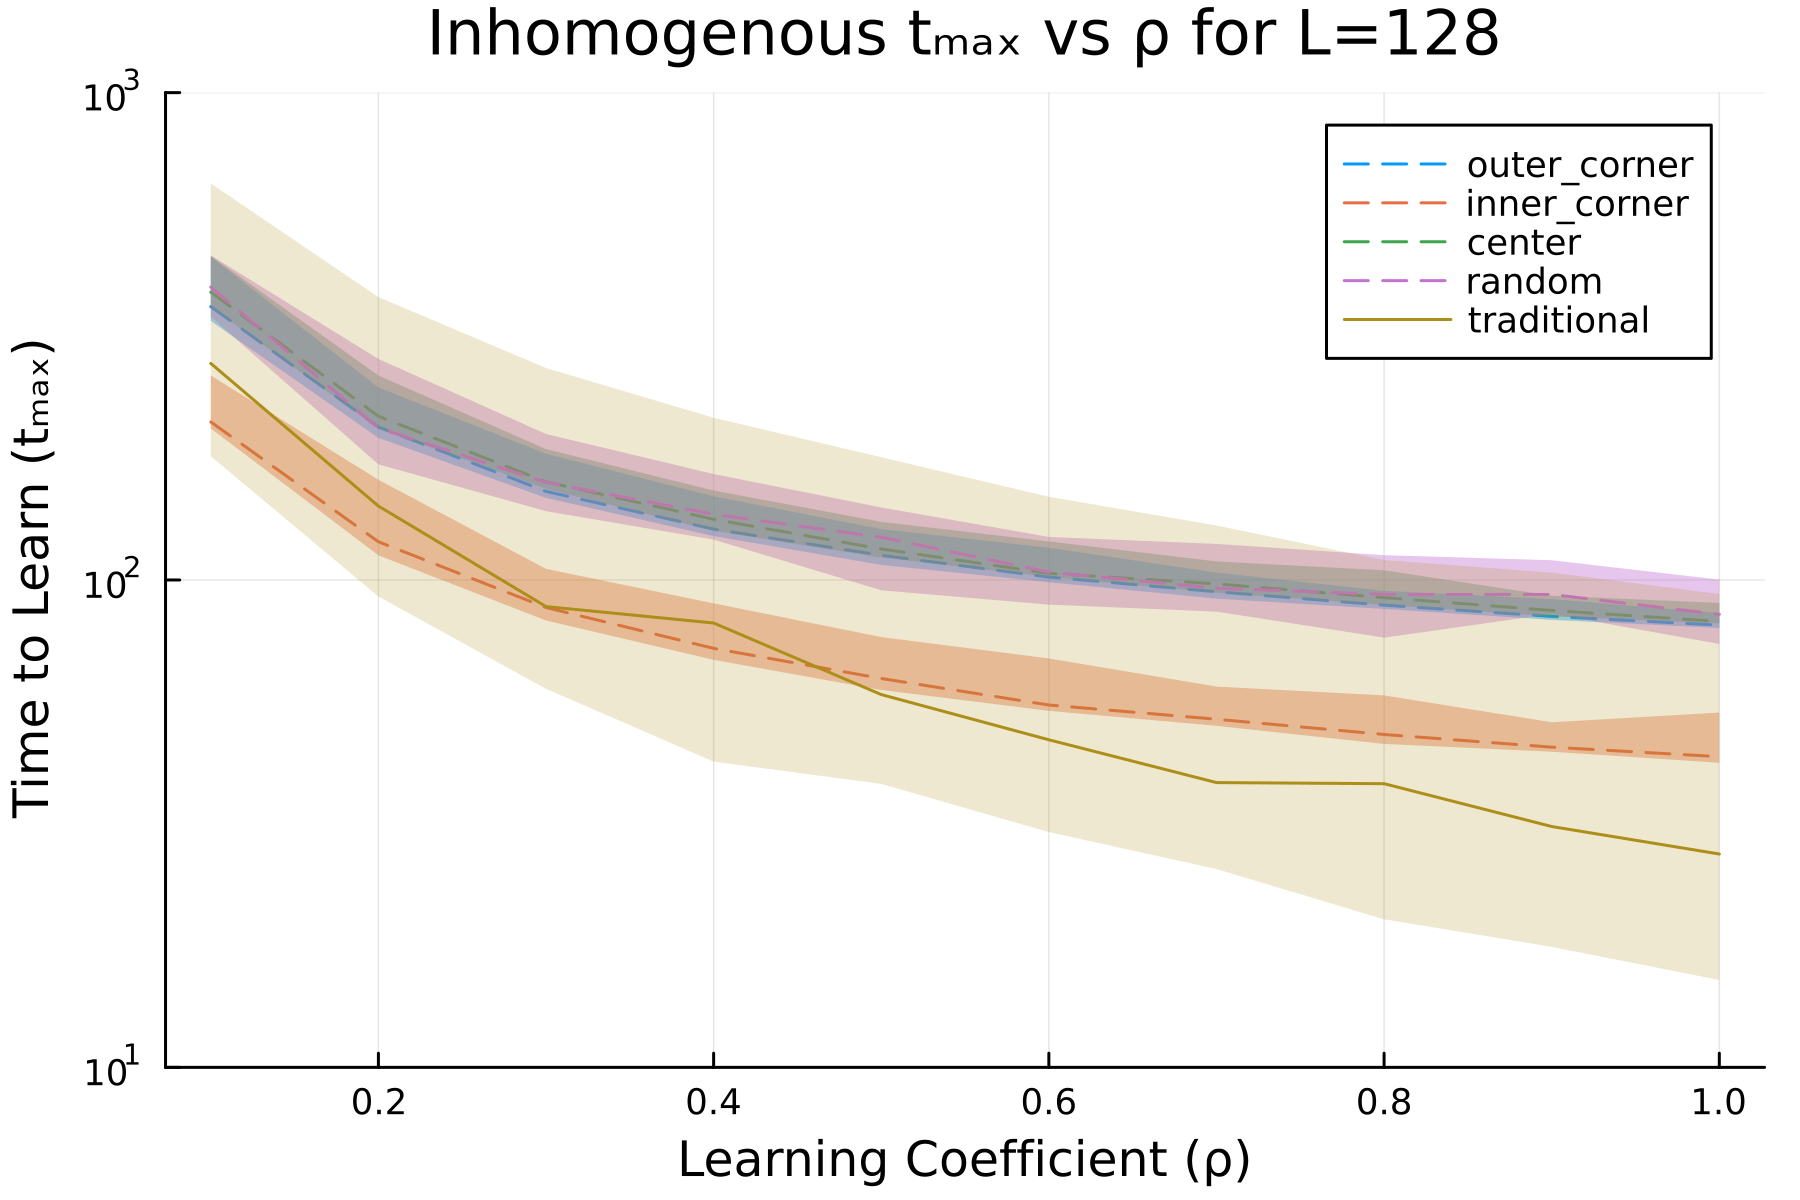
\includegraphics[width=0.49\textwidth]{figures/2D-BPCAIH-analysis/rho-t ribbon plots/rho-t-ribbon-128.png}}
   \caption[Positional learning factor $\rho_0$ dependence of time to learn $t_{max}$ for the heterogeneous classroom model for all SAs and classroom lengths $L$]{Time to learn $t_{max}$ as a function of positional learning factor $\rho_0$ for the heterogeneous model of all seating arrangements and classroom sizes $L$. 
   Each ribbon series represent the range of values for $t_{max}$ for a given seating arrangements with heterogeneity $\delta\lambda = \lbrace 0.0, 0.1, 0.2, 0.3, 0.4 \rbrace$.
   Lower time to learn $t_{max}$ indicates better performance.
   }
   \label{fig:2DBPCAIH t-rho ribbon plot}
\end{figure}

\newpage % new page after section t vs rho

\section{Time to learn $t_{max}$ vs heterogeneity $\delta\lambda$}\label{sec:BPCAIH t vs dl}

Figure~\ref{fig:2DBPCAIH dl-t plots} shows that as heterogeneity $\delta\lambda$ increases, PI methods perform better than traditional methods even when PI methods have lower positional learning factors $\rho_0$. For our representative $\rho_0$ values, PI performs better than traditional methods regardless of the $\rho_0$ value, even in a large classroom $L=128$. 
However, in larger classrooms, the advantage in performance of PI over traditional methods is less pronounced. 
Furthermore, as class size increases, traditional methods tend to stay advantageous than PI methods for increasing values of heterogeneity $\delta\lambda$.

For example, at $L=32$ shown in figure \ref{fig:2DBPCAIH dl-t plot 32}, PI methods are better than traditional methods for all values of $\delta\lambda$ when comparing between equal $\rho_0$ values. 
However, at $L=128$ shown in figure \ref{fig:2DBPCAIH dl-t plot 128}, the traditional model performs better than the PI model for $0 \leq \delta\lambda \leq 0.2$ when comparing between equal $\rho_0$ values.

\begin{figure}[htbp!]
   \centering
   \subfigure[$L=32$]{\label{fig:2DBPCAIH dl-t plot 32}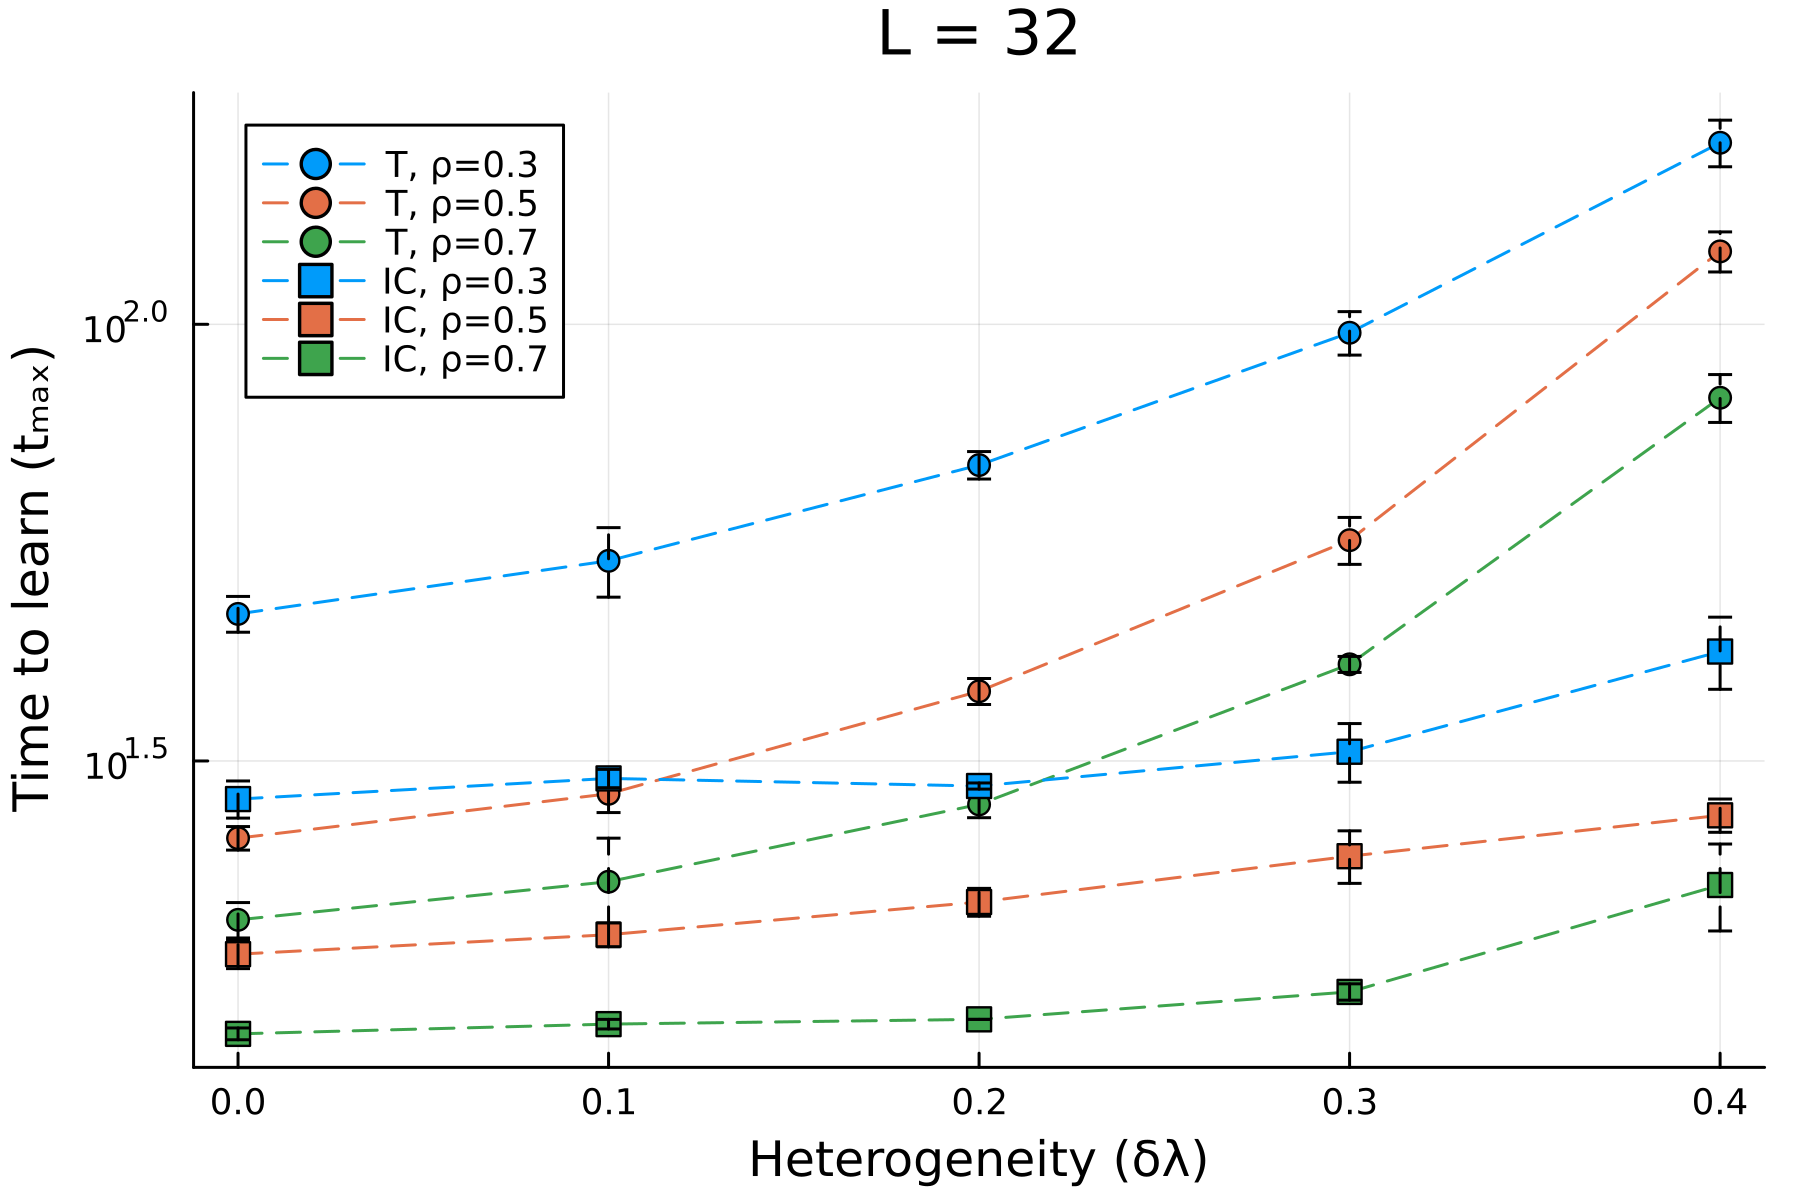
\includegraphics[width=0.49\textwidth]{figures/2D-BPCAIH-analysis/dl-t plots/dl-t-32.png}}
   \subfigure[$L=128$]{\label{fig:2DBPCAIH dl-t plot 128}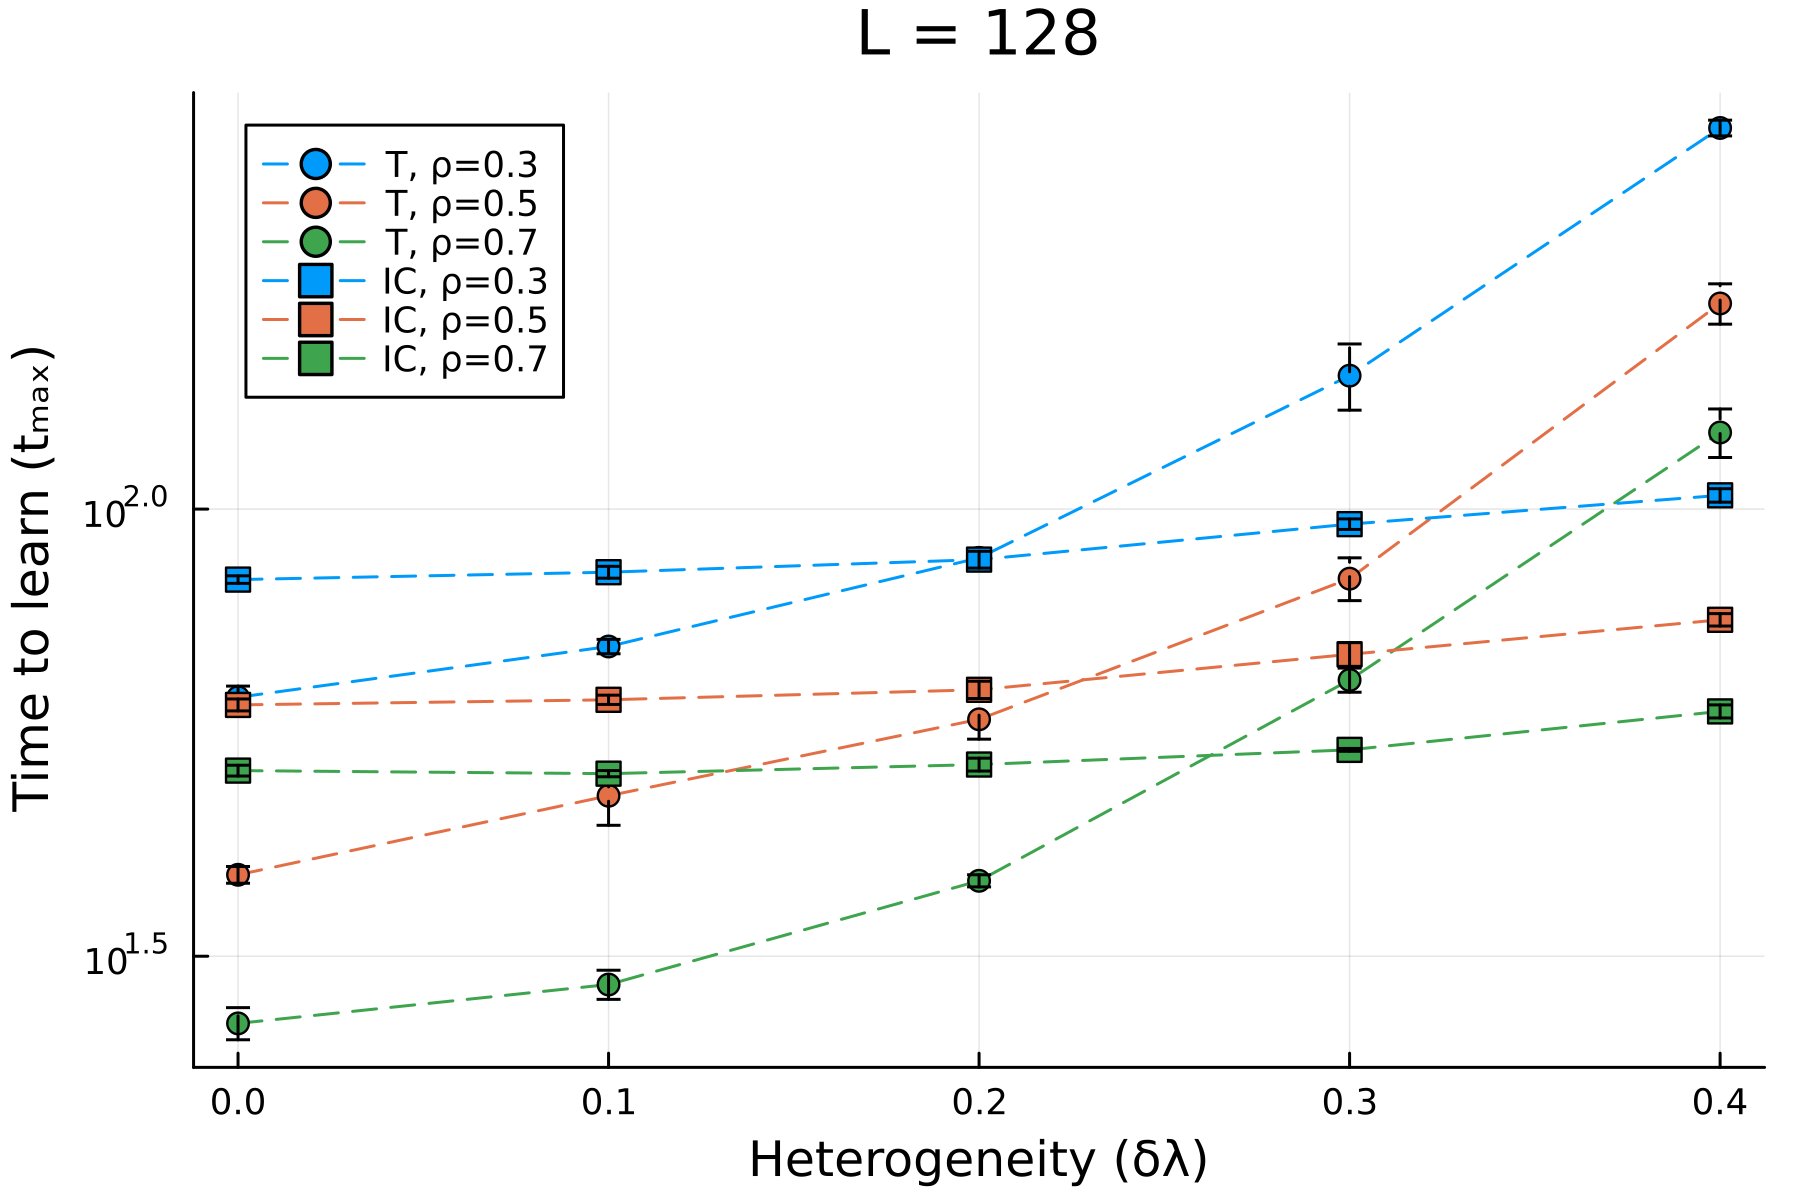
\includegraphics[width=0.49\textwidth]{figures/2D-BPCAIH-analysis/dl-t plots/dl-t-128.png}}
   \caption[Heterogeneity $\delta\lambda$ dependence of time to learn $t_{max}$ for the heterogeneous classroom model]{Time to learn $t_{max}$ as a function of heterogeneity $\delta\lambda$ for the heterogeneous models of the PI (inner corner SA) and traditional models with varying positional learning factor $\rho_0\in\lbrace 0.3,0.5,0.7 \rbrace$ and classroom sizes $L\in\lbrace32,128\rbrace$. 
   Each color represents a different value of $\rho_0$, while the circle and square symbols represent the traditional and PI models respectively.
   Lower time to learn $t_{max}$ indicates better performance.
   }
   \label{fig:2DBPCAIH dl-t plots}
\end{figure}

\newpage % new page after section t vs dl

\section{Time to learn $t_{max}$ vs class size $N$}\label{sec:BPCAIH m vs dl}

When investigating the size dependence of time to learn $t_{max}$ shown in Figure~\ref{fig:2DBPCAIH n-t plots}, we see a similar trend to what we found in section \ref{subsec: 2DBPCA tmax vs N} where PI models are better for smaller classes and traditional models are better for larger classes.
Heterogeneity $\delta\lambda$ generally has a negative effect on the time to learn $t_{max}$ for both PI and traditional models.
However, as shown in sections \ref{sec:BPCAIH t vs rho} and \ref{sec:BPCAIH t vs dl}, the traditional model is more affected by heterogeneity $\delta\lambda$ compared to PI models.
Because of the sensitivity of traditional instruction to heterogeneity $\delta\lambda$, at low values of $\rho_0$, even for large classes, PI models can perform better than traditional models for higher values of heterogeneity $\delta\lambda$.
This is shown in Figures \ref{fig:2DBPCAIH n-t plot 0.3} and \ref{fig:2DBPCAIH n-t plot 0.4} where the PI model performs better than the traditional model for all class sizes (N) and the same value of $\rho_0$.

\begin{figure}[htbp!]
   \centering
   \subfigure[$\delta\lambda=0.0$]{\label{fig:2DBPCAIH n-t plot 0.0}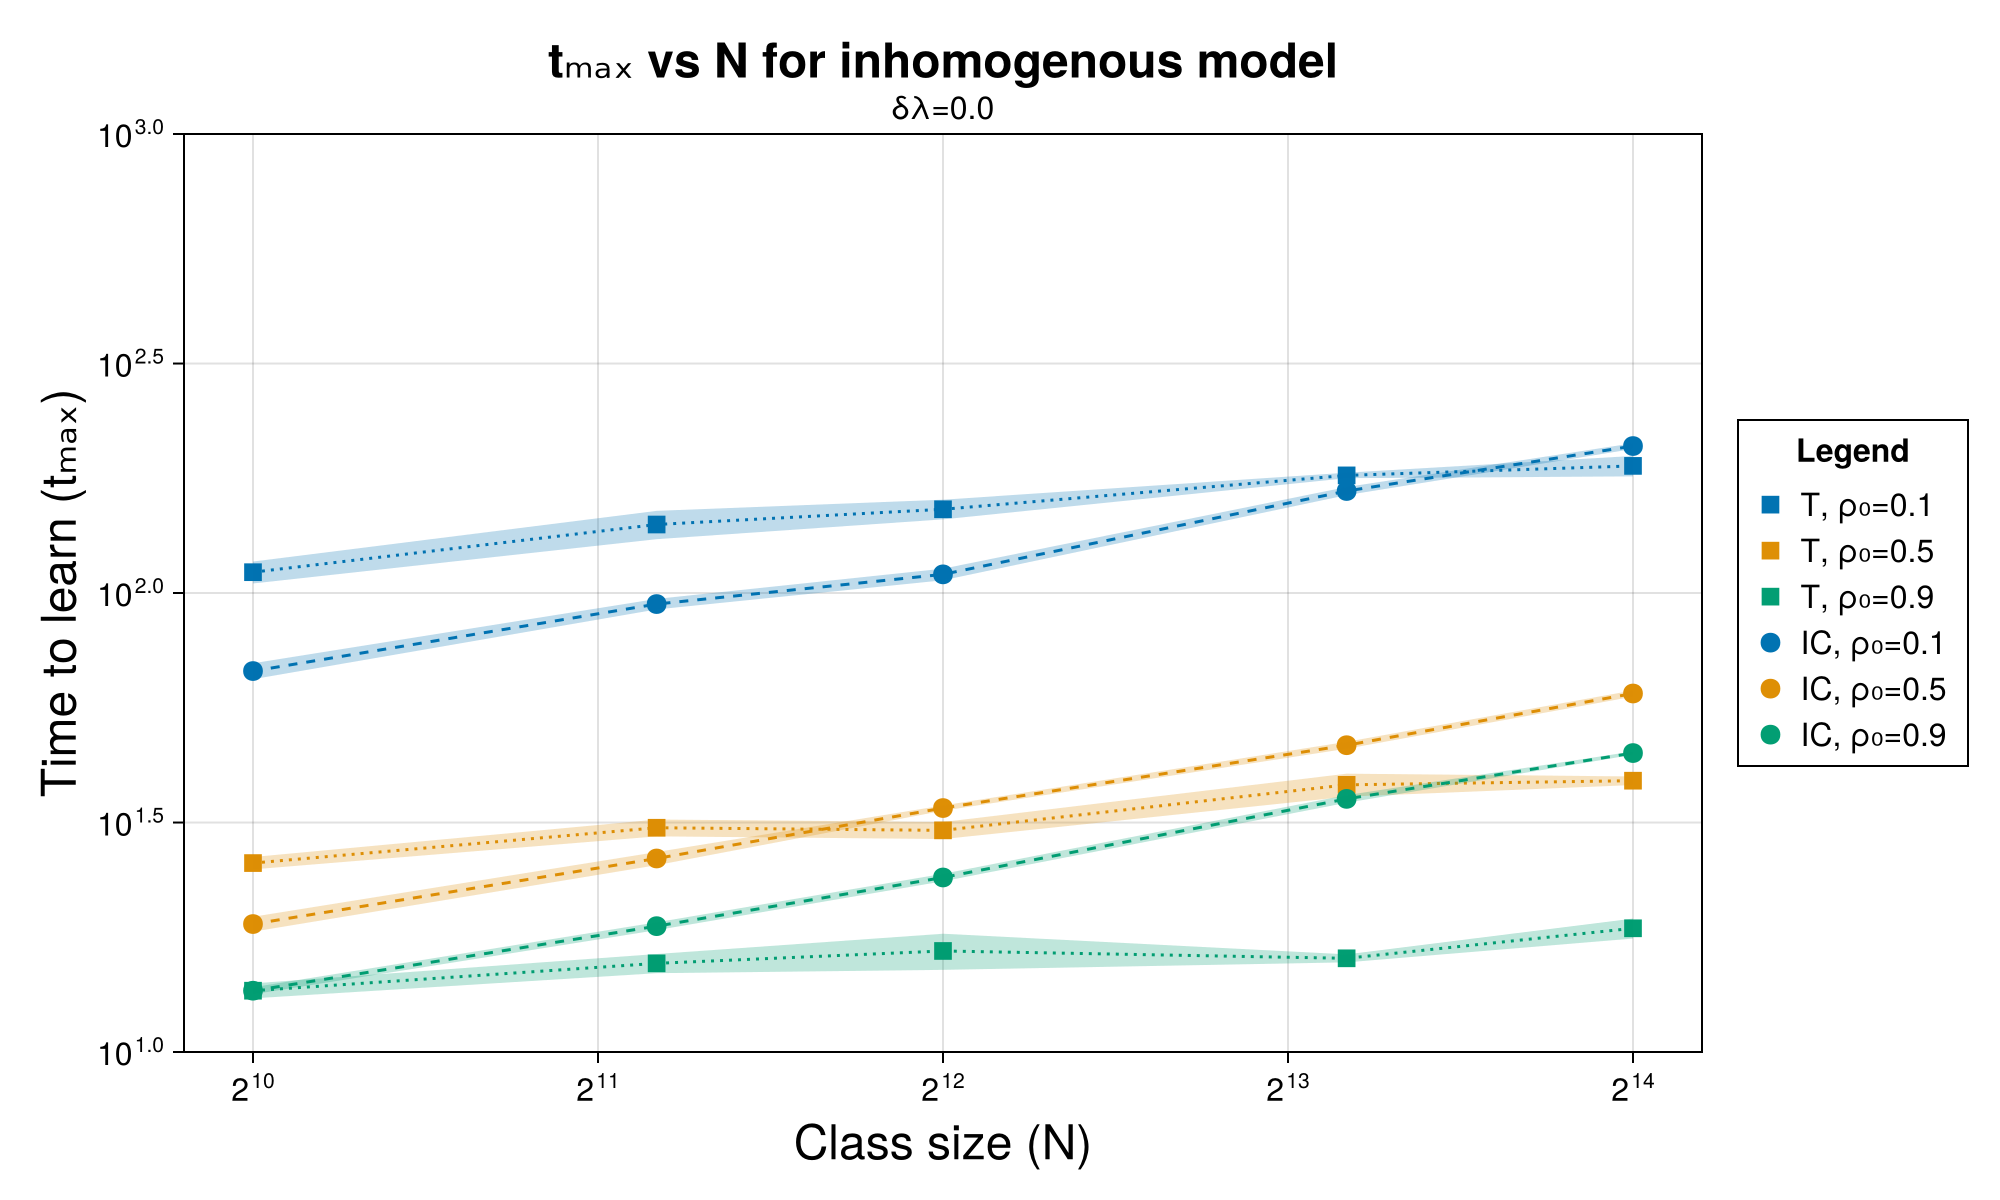
\includegraphics[width=0.49\textwidth]{figures/2D-BPCAIH-analysis/n-t plots/n-t-plot-0.0.png}}
   \subfigure[$\delta\lambda=0.1$]{\label{fig:2DBPCAIH n-t plot 0.1}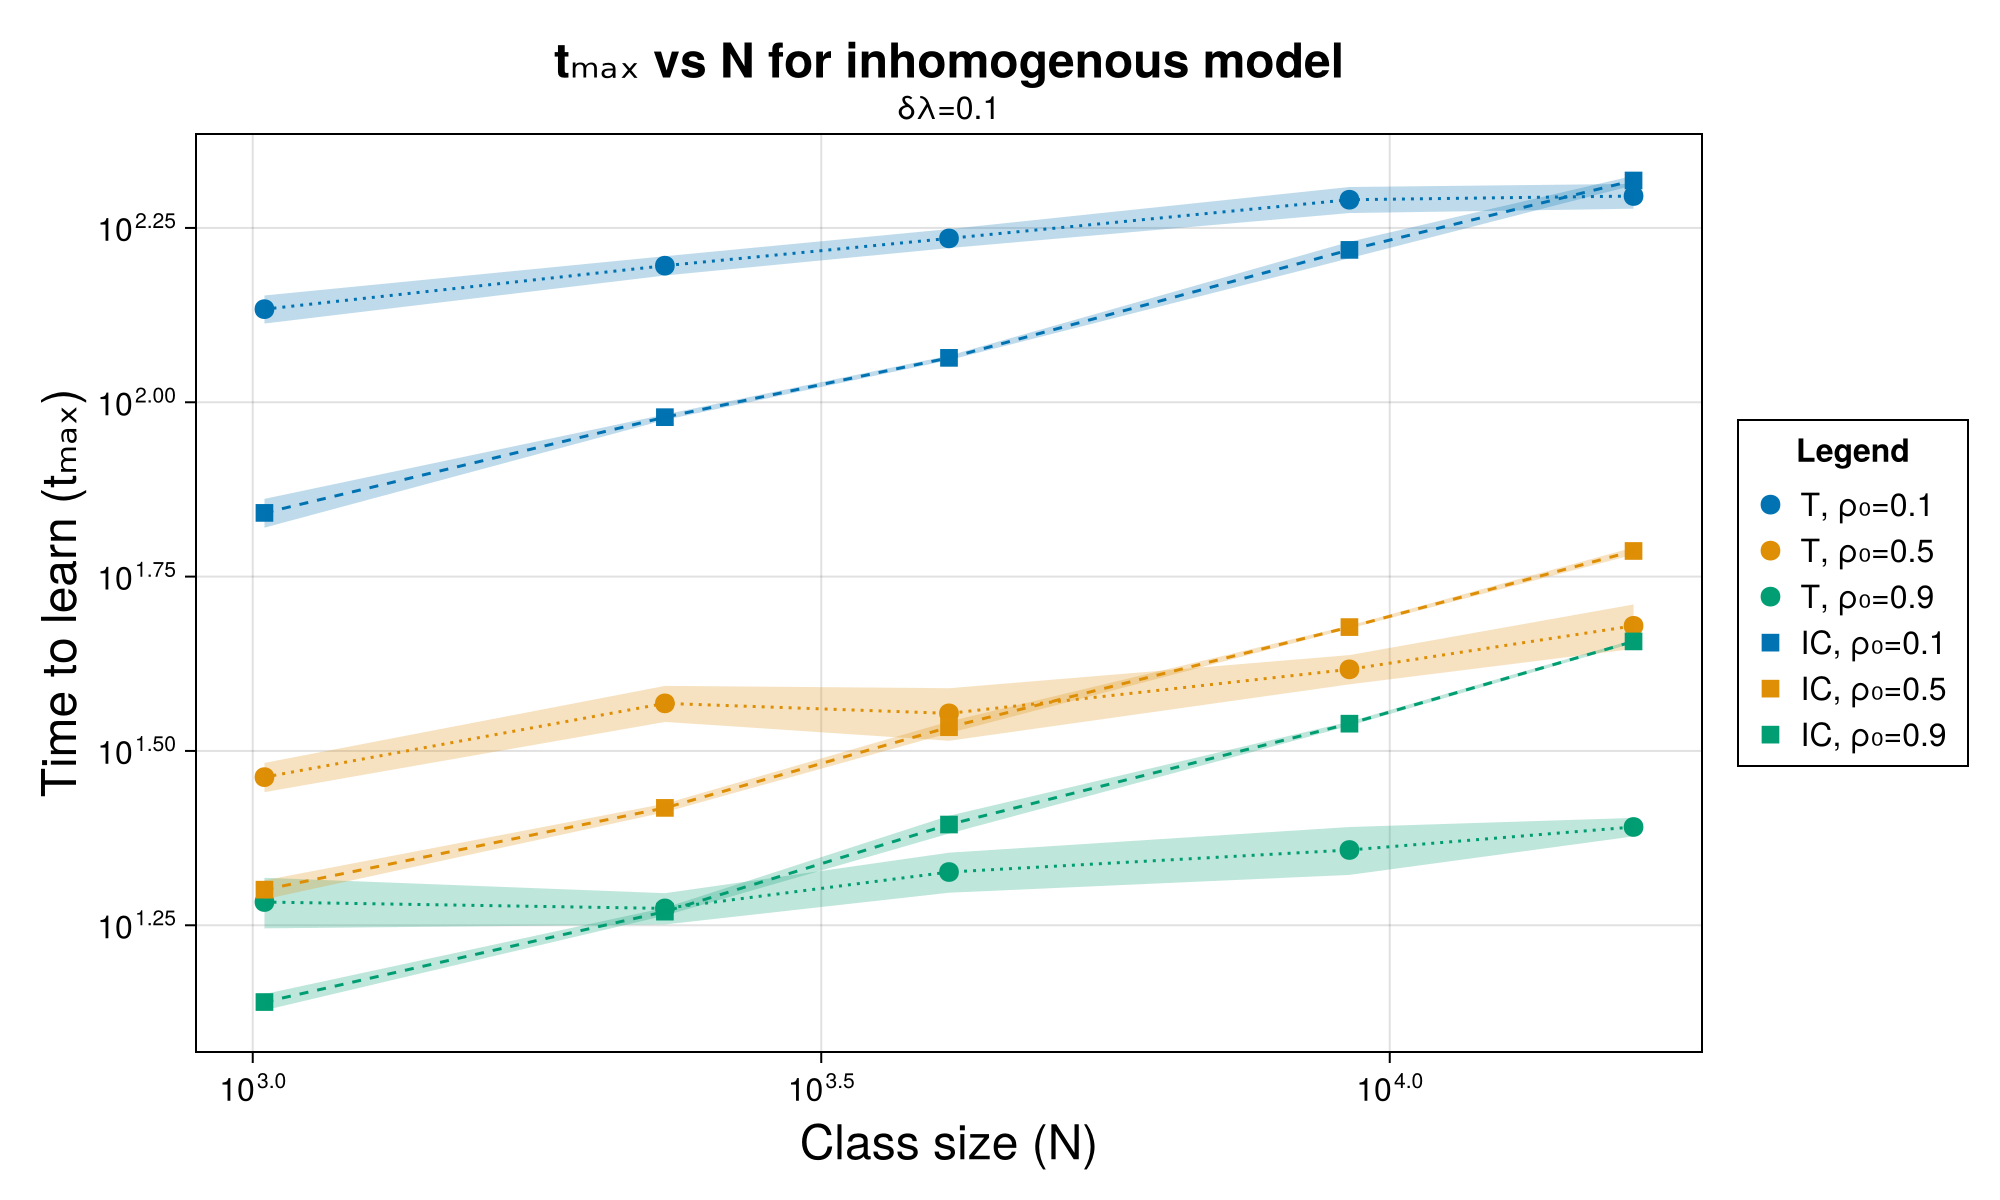
\includegraphics[width=0.49\textwidth]{figures/2D-BPCAIH-analysis/n-t plots/n-t-plot-0.1.png}}
   \subfigure[$\delta\lambda=0.2$]{\label{fig:2DBPCAIH n-t plot 0.2}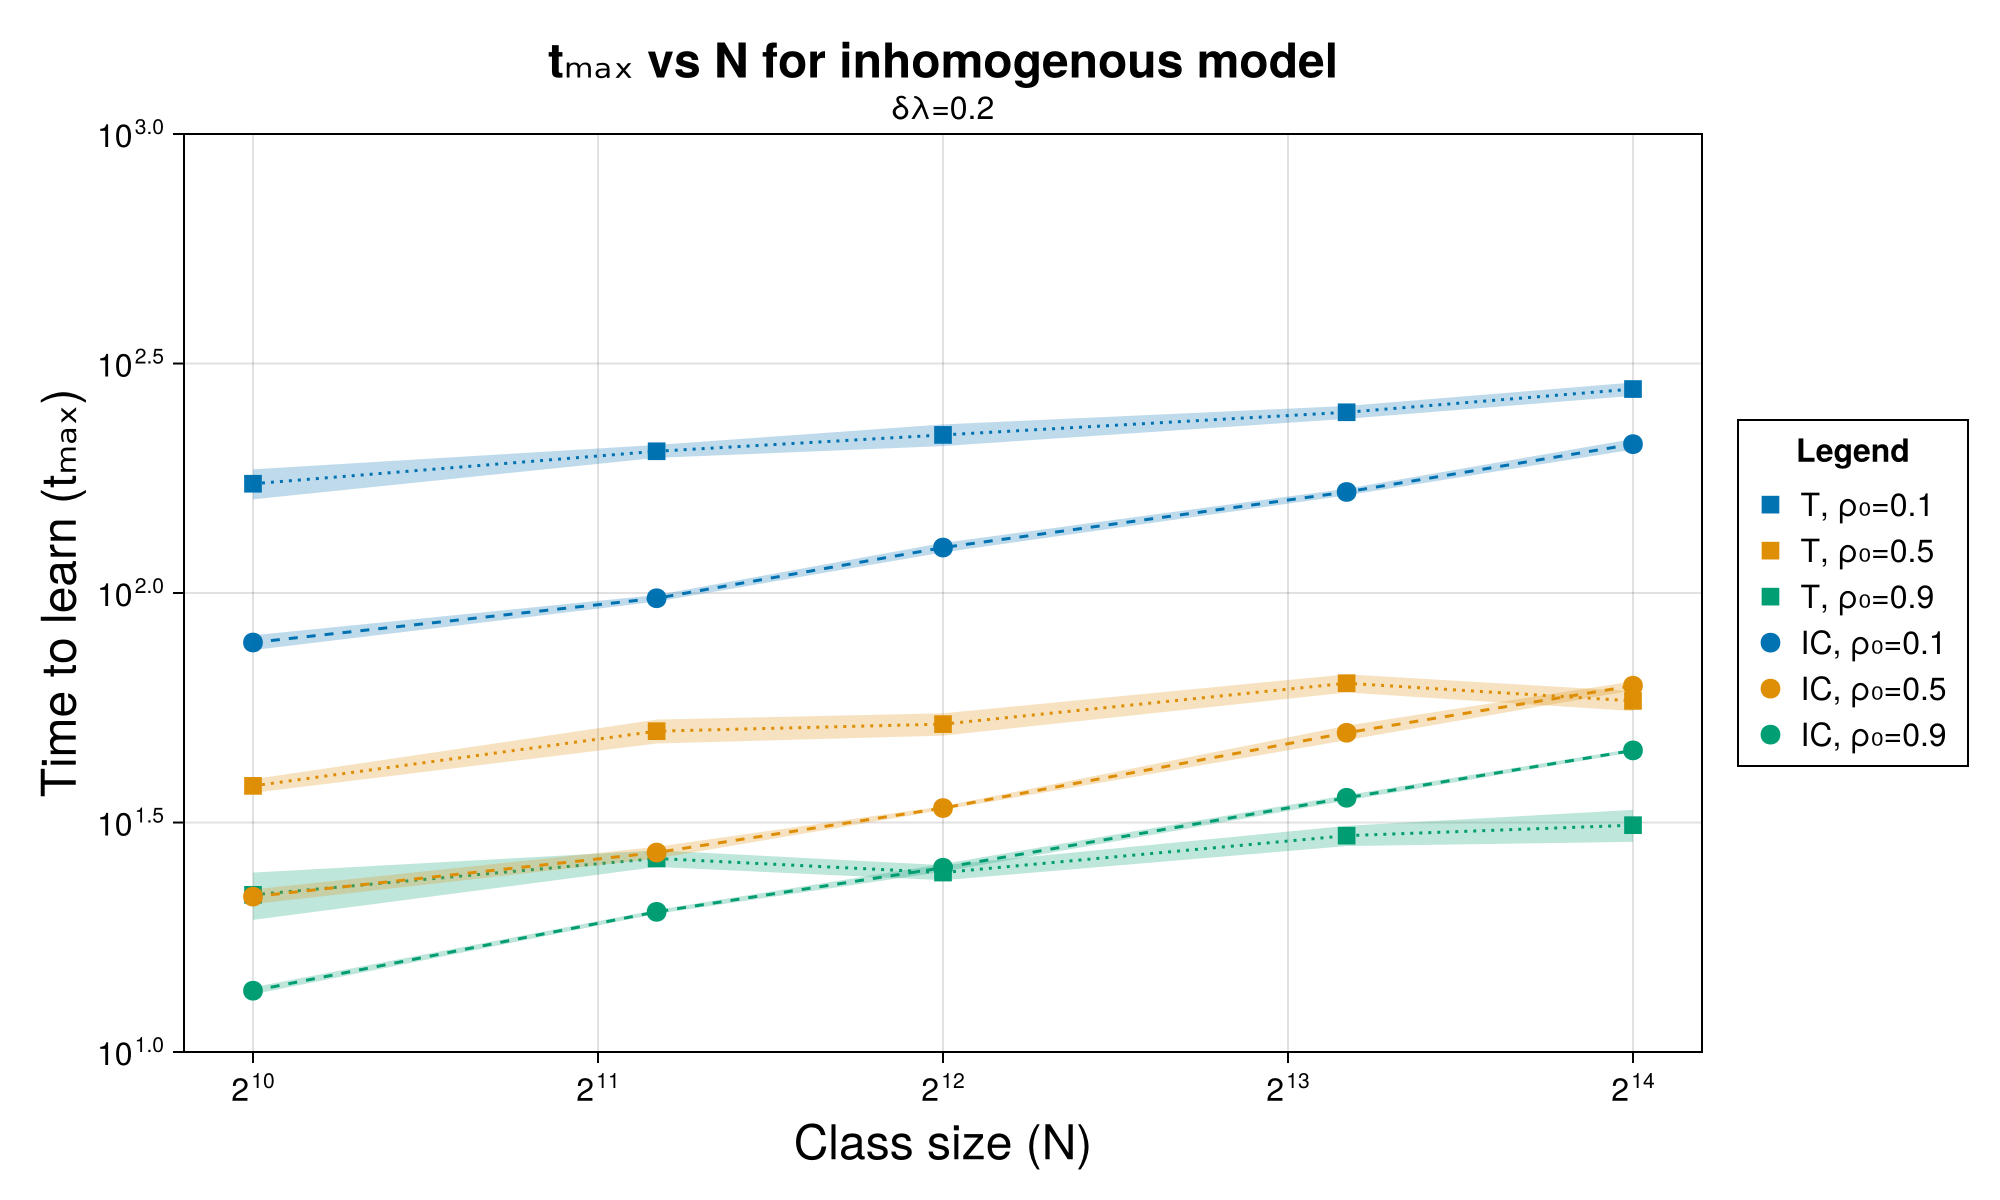
\includegraphics[width=0.49\textwidth]{figures/2D-BPCAIH-analysis/n-t plots/n-t-plot-0.2.png}}
   \subfigure[$\delta\lambda=0.3$]{\label{fig:2DBPCAIH n-t plot 0.3}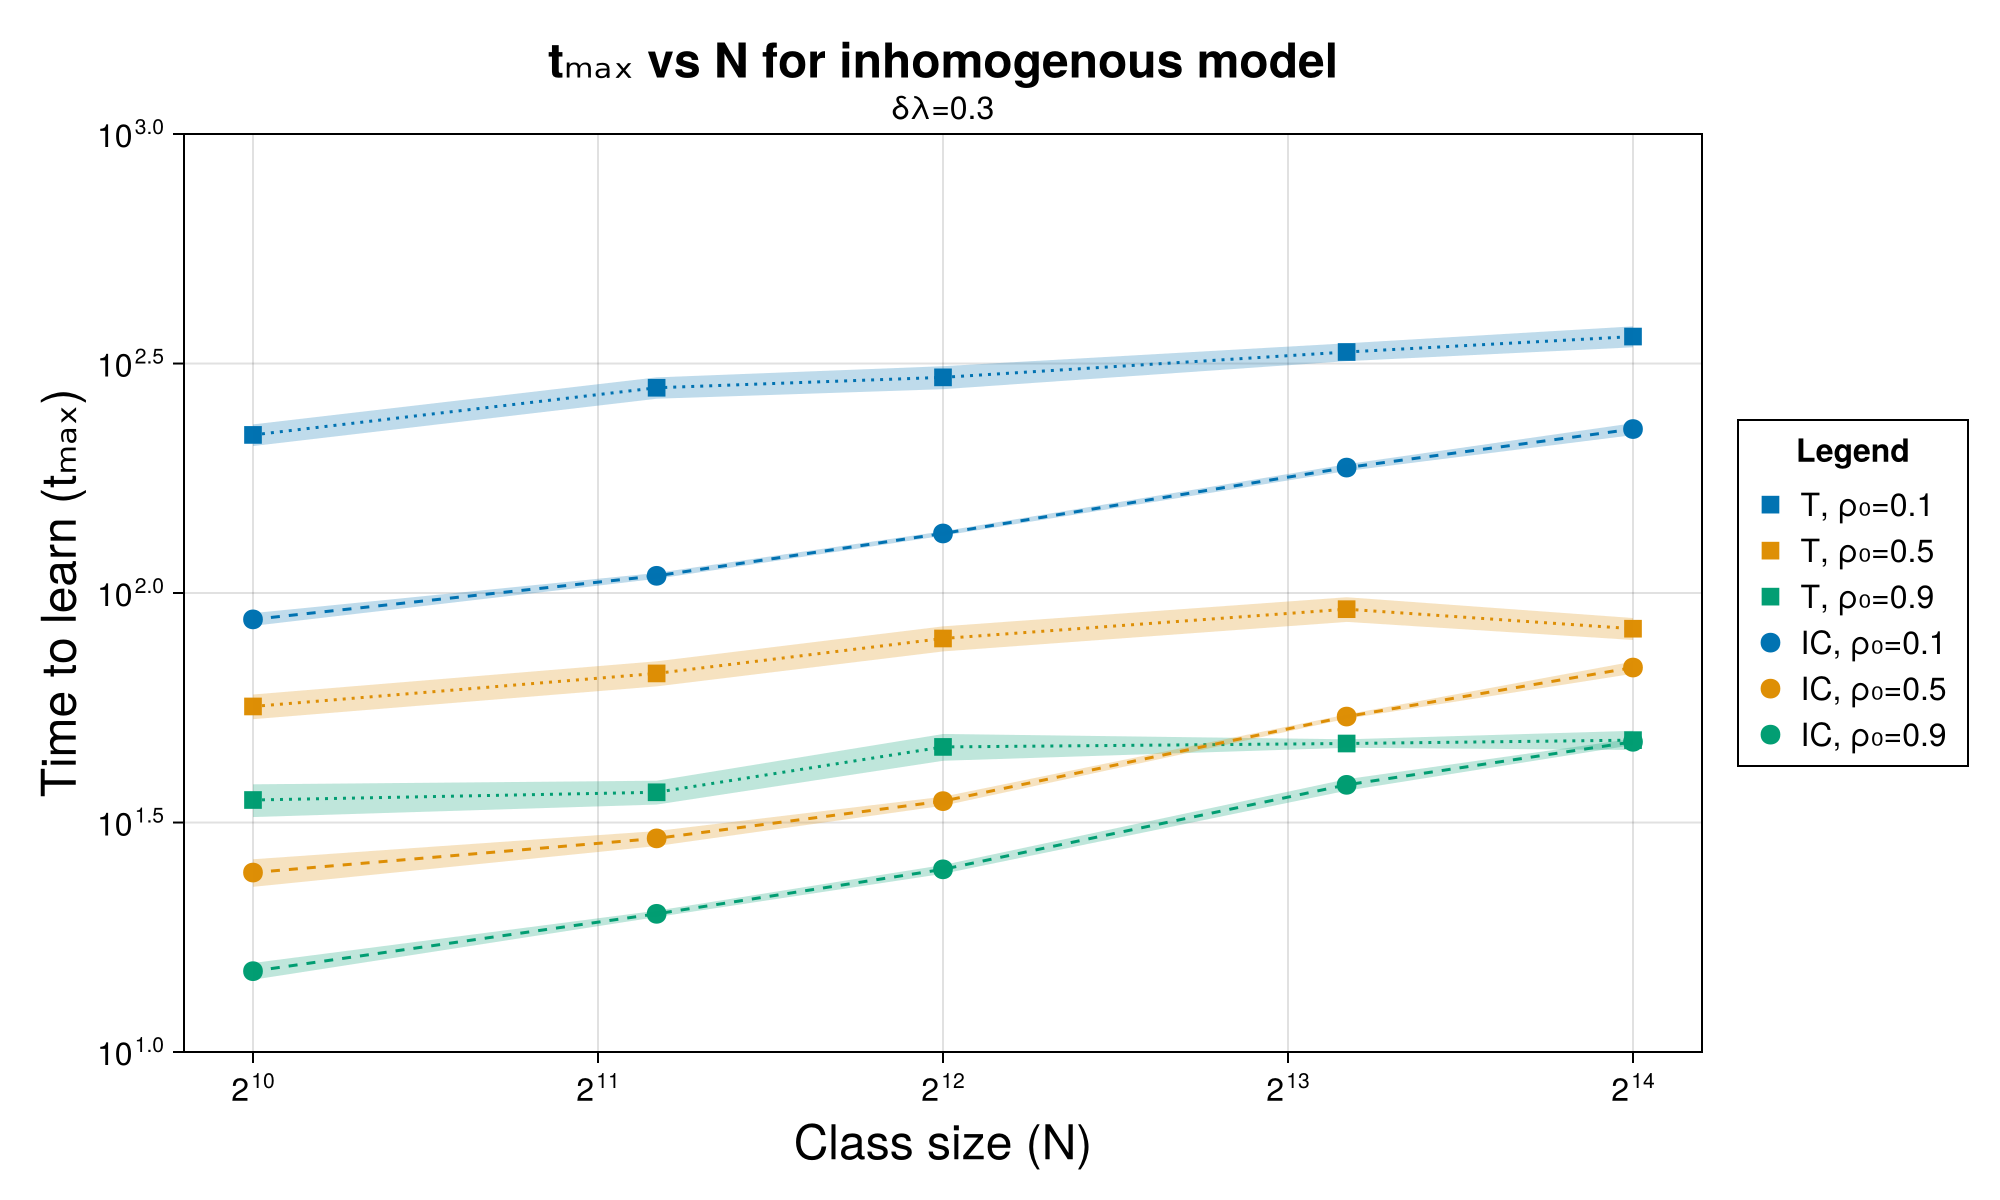
\includegraphics[width=0.49\textwidth]{figures/2D-BPCAIH-analysis/n-t plots/n-t-plot-0.3.png}}
   \subfigure[$\delta\lambda=0.4$]{\label{fig:2DBPCAIH n-t plot 0.4}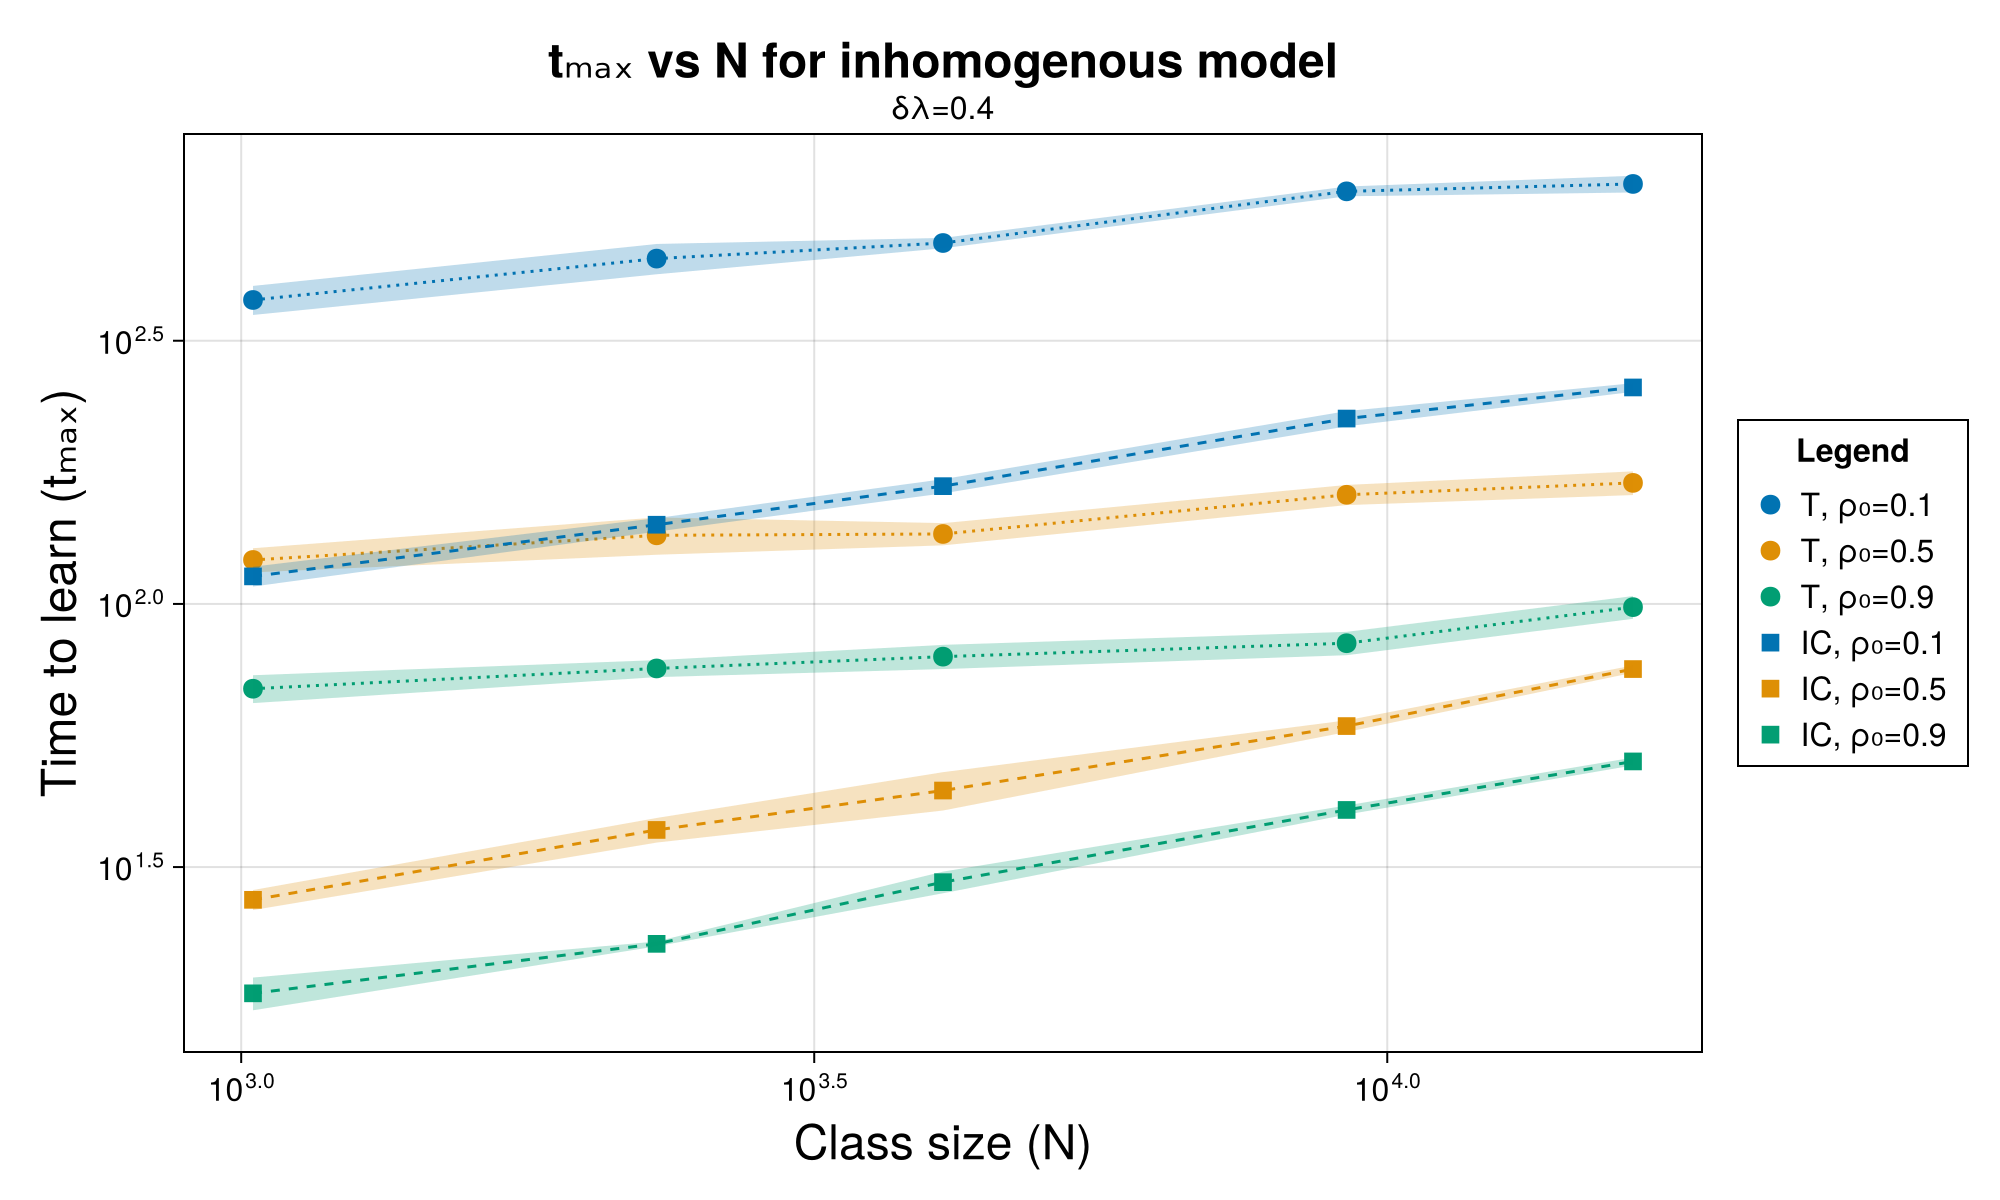
\includegraphics[width=0.49\textwidth]{figures/2D-BPCAIH-analysis/n-t plots/n-t-plot-0.4.png}}
   \caption[Class size $N$ dependence of time to learn $t_{max}$ for the heterogeneous classroom model]{Time to learn $t_{max}$ as a function of class size $N$ for the heterogeneous models of the PI (inner corner SA) and traditional models with varying positional learning factor $\rho_0\in\lbrace 0.1, 0.5, 0.9 \rbrace$ and heterogeneity $\delta\lambda\in\lbrace0.0, 0.1, 0.2, 0.3, 0.4 \rbrace$. 
   Each color represents a different value of $\rho_0$, while the circle and square symbols represent the traditional and PI models respectively.
   Each band represents the standard deviation of time to learn $t_{max}$ over 5 trials.
   Lower time to learn $t_{max}$ indicates better performance.
   }
   \label{fig:2DBPCAIH n-t plots}
\end{figure}

\newpage % new page after section t vs N

\section{An overview of the different parameters that affect time to learn $t_{max}$}\label{sec:BPCAIH 3D plots}

Figure~\ref{fig:2DBPCAIH rho-dl-t plots} gives us a better visualization of the relationships between the positional learning factor $\rho_0$, heterogeneity $\delta\lambda$, and time to learn $t_{max}$ for the PI and traditional models.
In addition to our previous findings in Sections~\ref{sec:BPCAIH t vs rho} and \ref{sec:BPCAIH t vs dl}, we see that PI is the safe choice between the two instruction modes regardless of the class conditions.
When traditional instruction is better than PI, there is not much of a difference in the time to learn $t_{max}$.
However, when PI performs better than traditional instruction, there are cases where the time to learn $t_{max}$ is significantly lower for PI compared to traditional instruction.

We also see that as $N=L^2$ increases, the trends for the time to learn $t_{max}$ remain consistent, with the biggest difference being  the shifting of the blue surface for PI upwards.

It should be noted that while the z-axis of the plots shown in Figure~\ref{fig:2DBPCAIH rho-dl-t plots} do not have the same limits, the grid lines remain consistent having the same interval of 100 time steps between each grid line.

\begin{figure}[htbp!]
   \centering
   \subfigure[$L=32$]{\label{fig:2DBPCAIH rho-dl-t plot 32}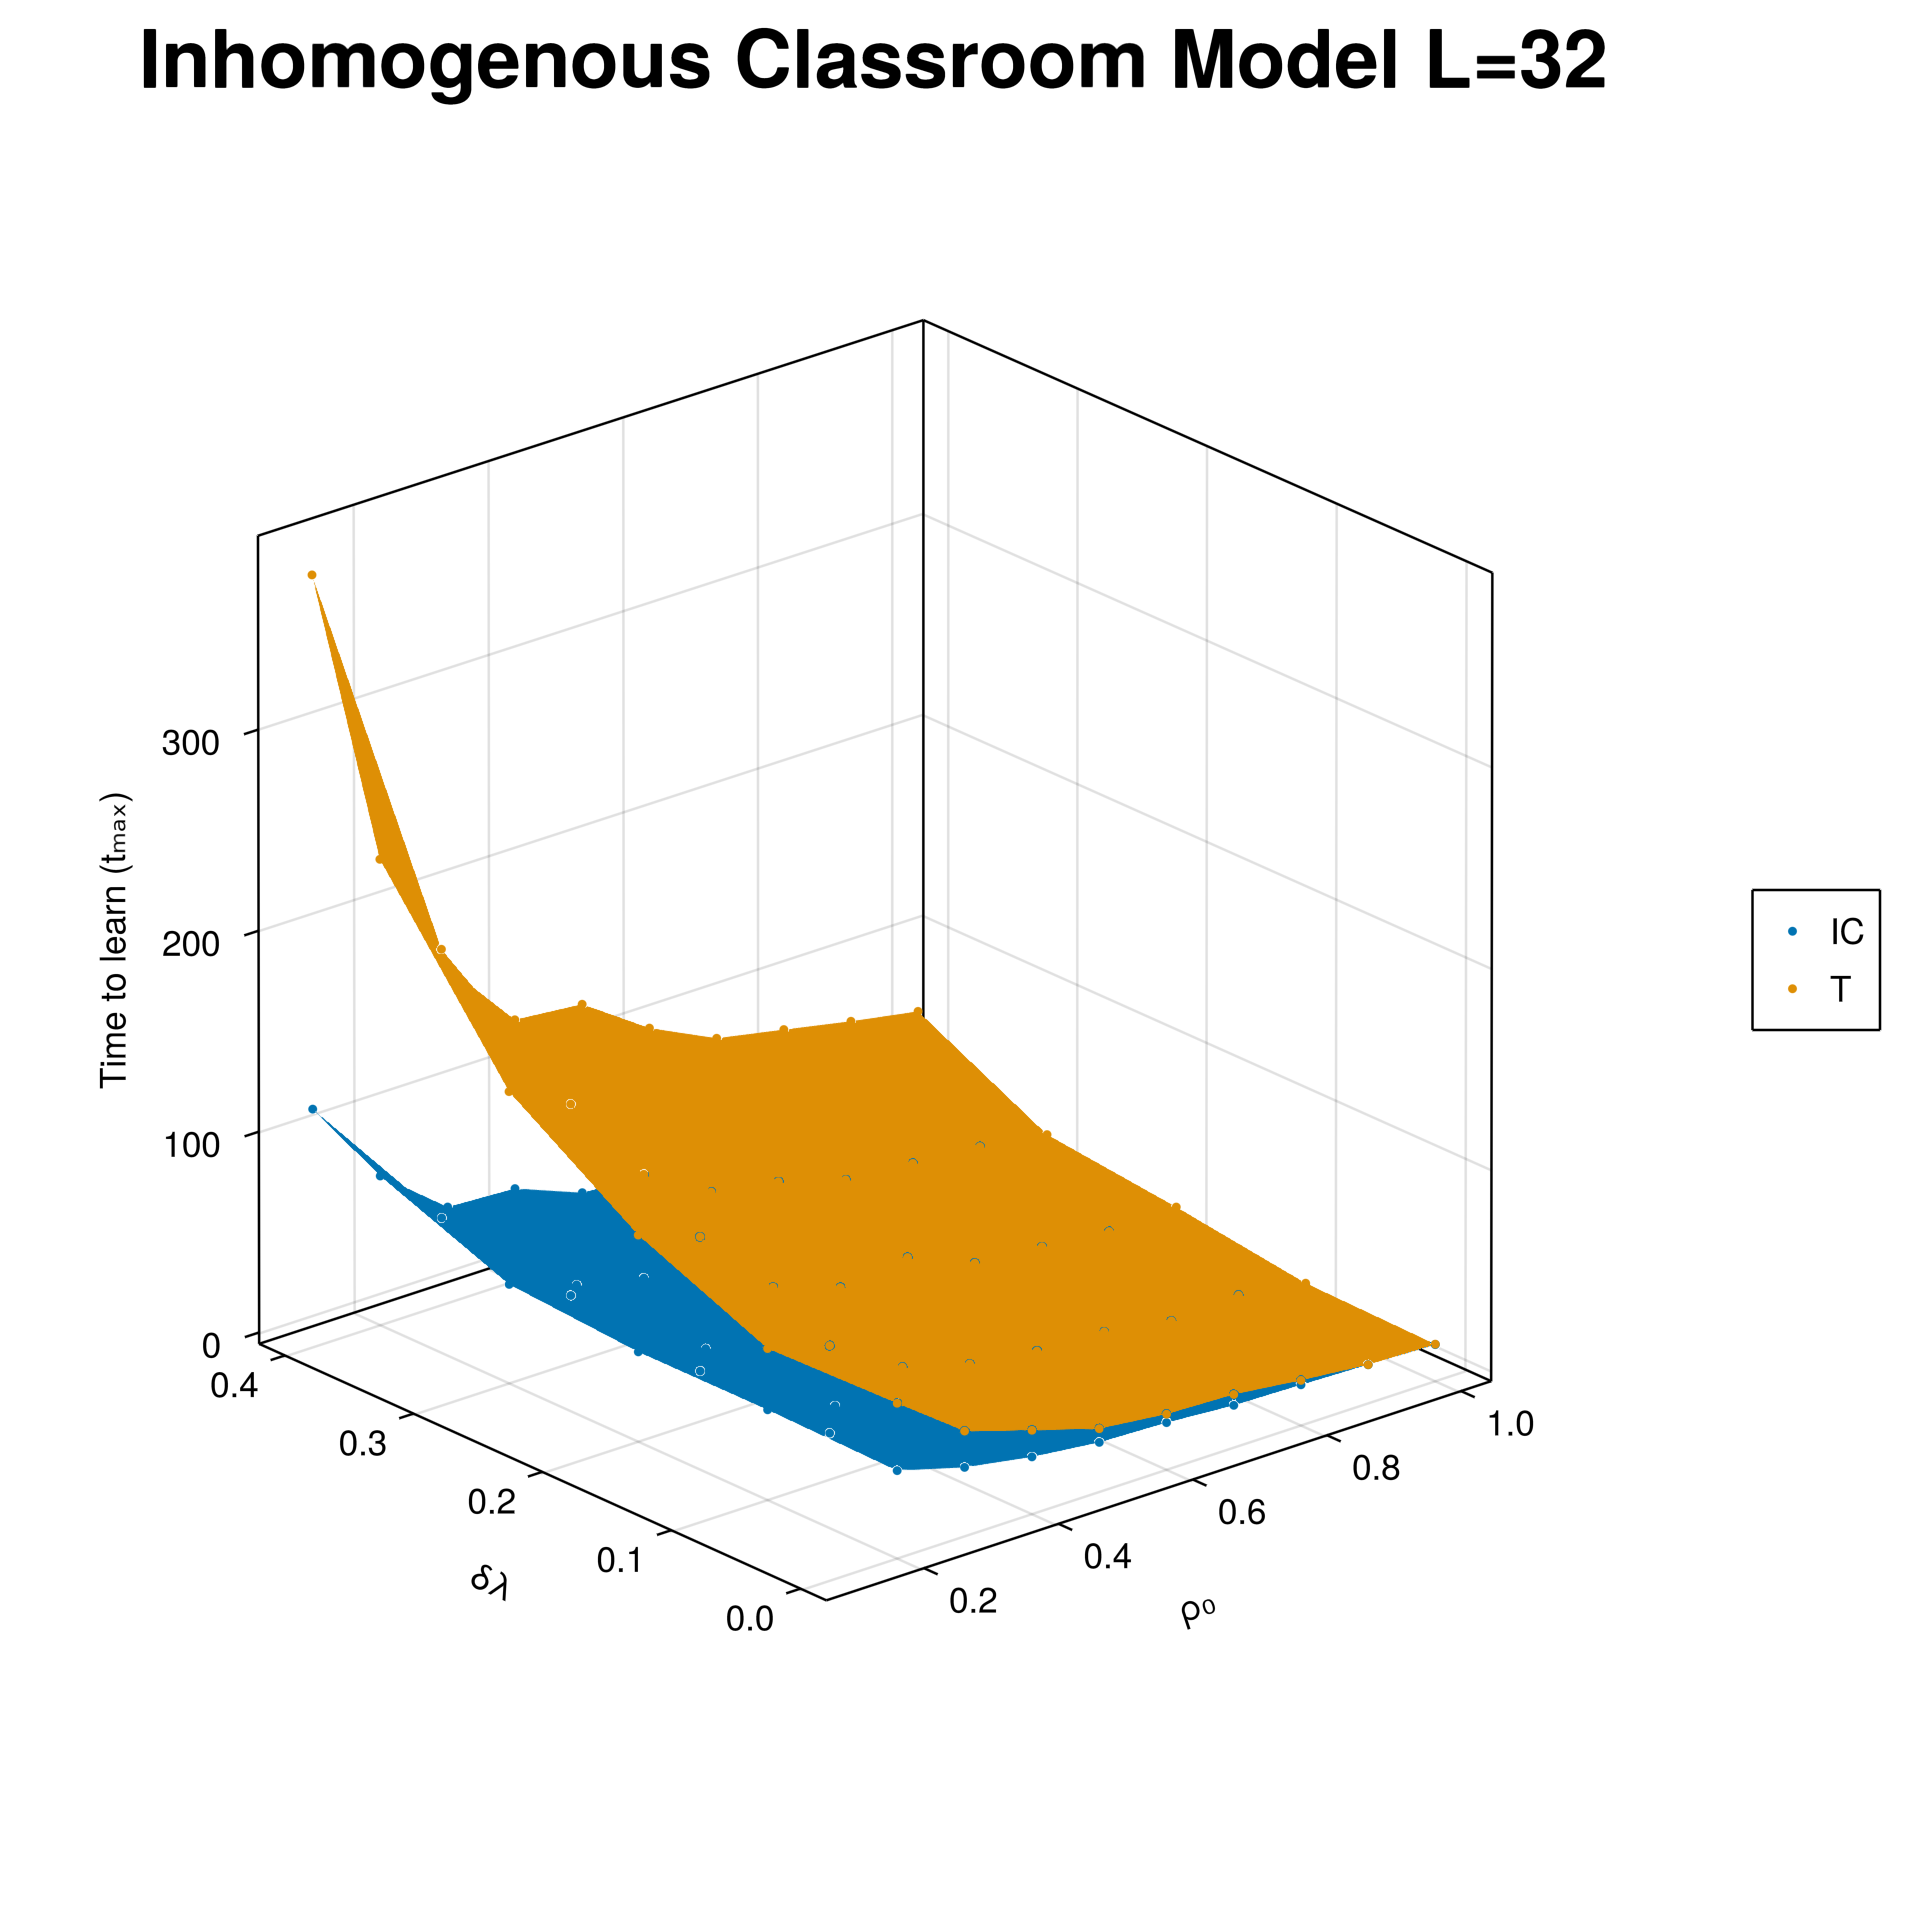
\includegraphics[width=0.40\textwidth]{figures/2D-BPCAIH-analysis/rho-dl-t plots/32.png}}
   \subfigure[$L=48$]{\label{fig:2DBPCAIH rho-dl-t plot 48}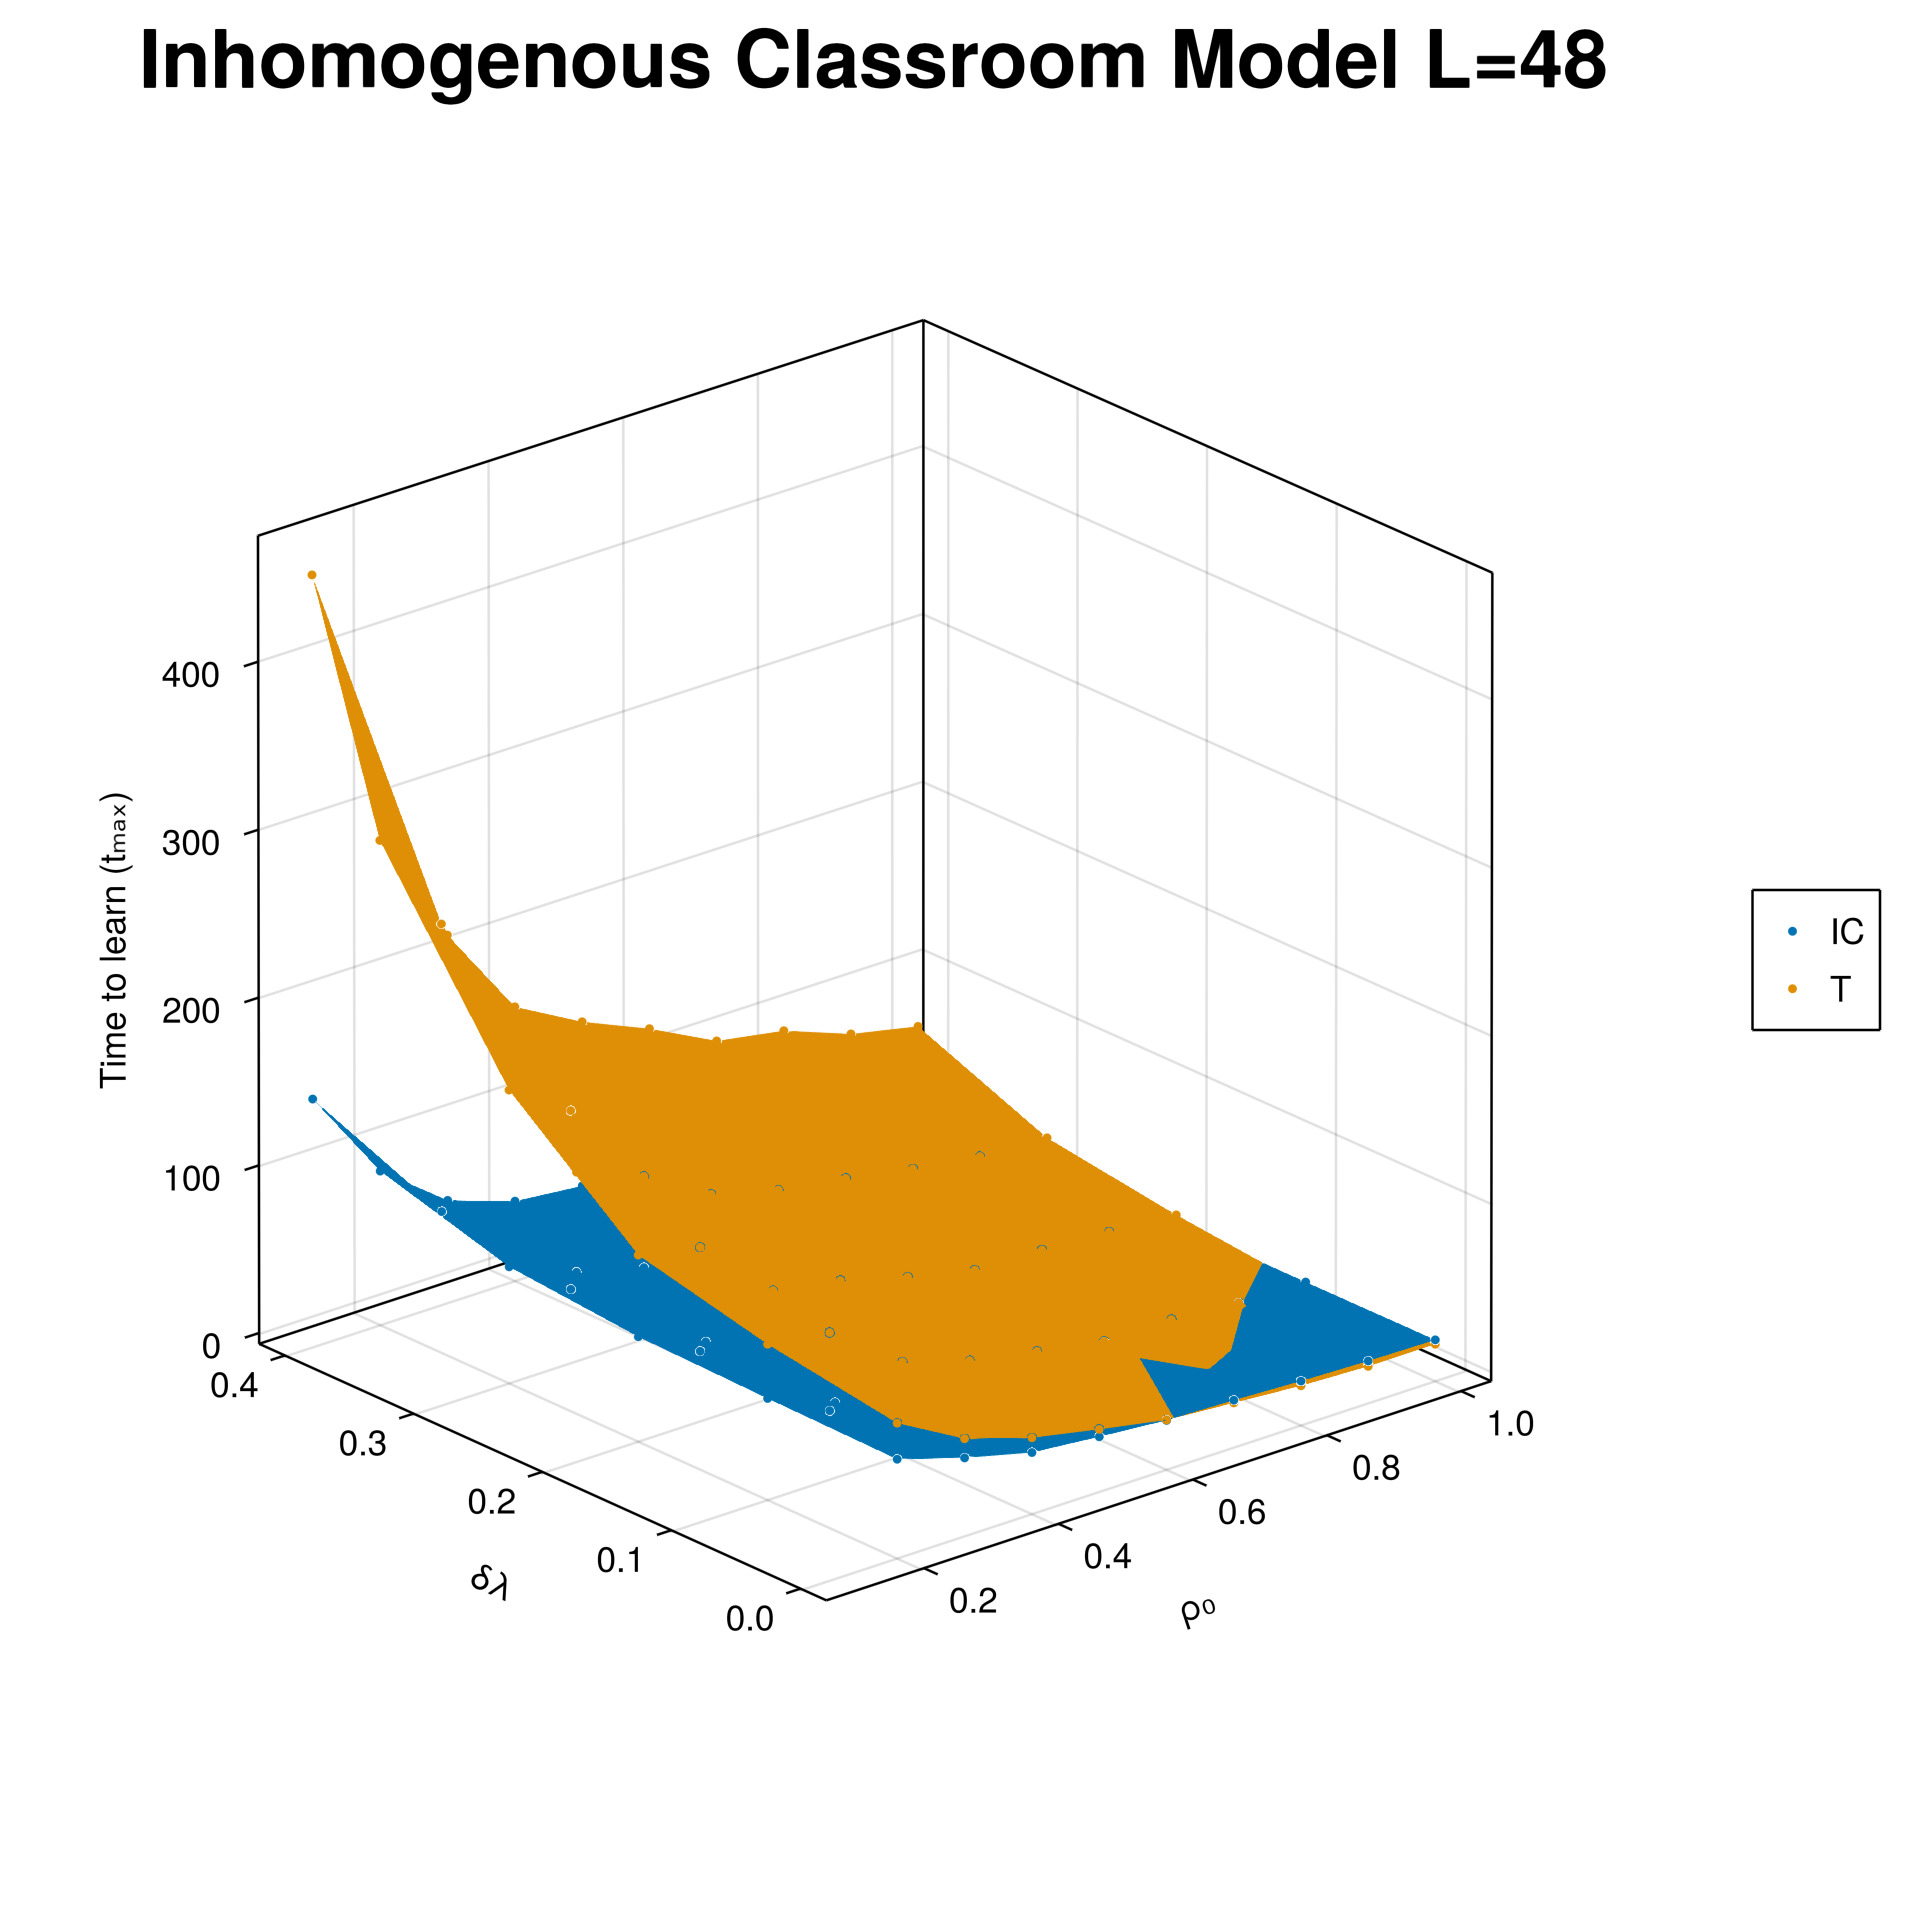
\includegraphics[width=0.40\textwidth]{figures/2D-BPCAIH-analysis/rho-dl-t plots/48.png}}
   \subfigure[$L=64$]{\label{fig:2DBPCAIH rho-dl-t plot 64}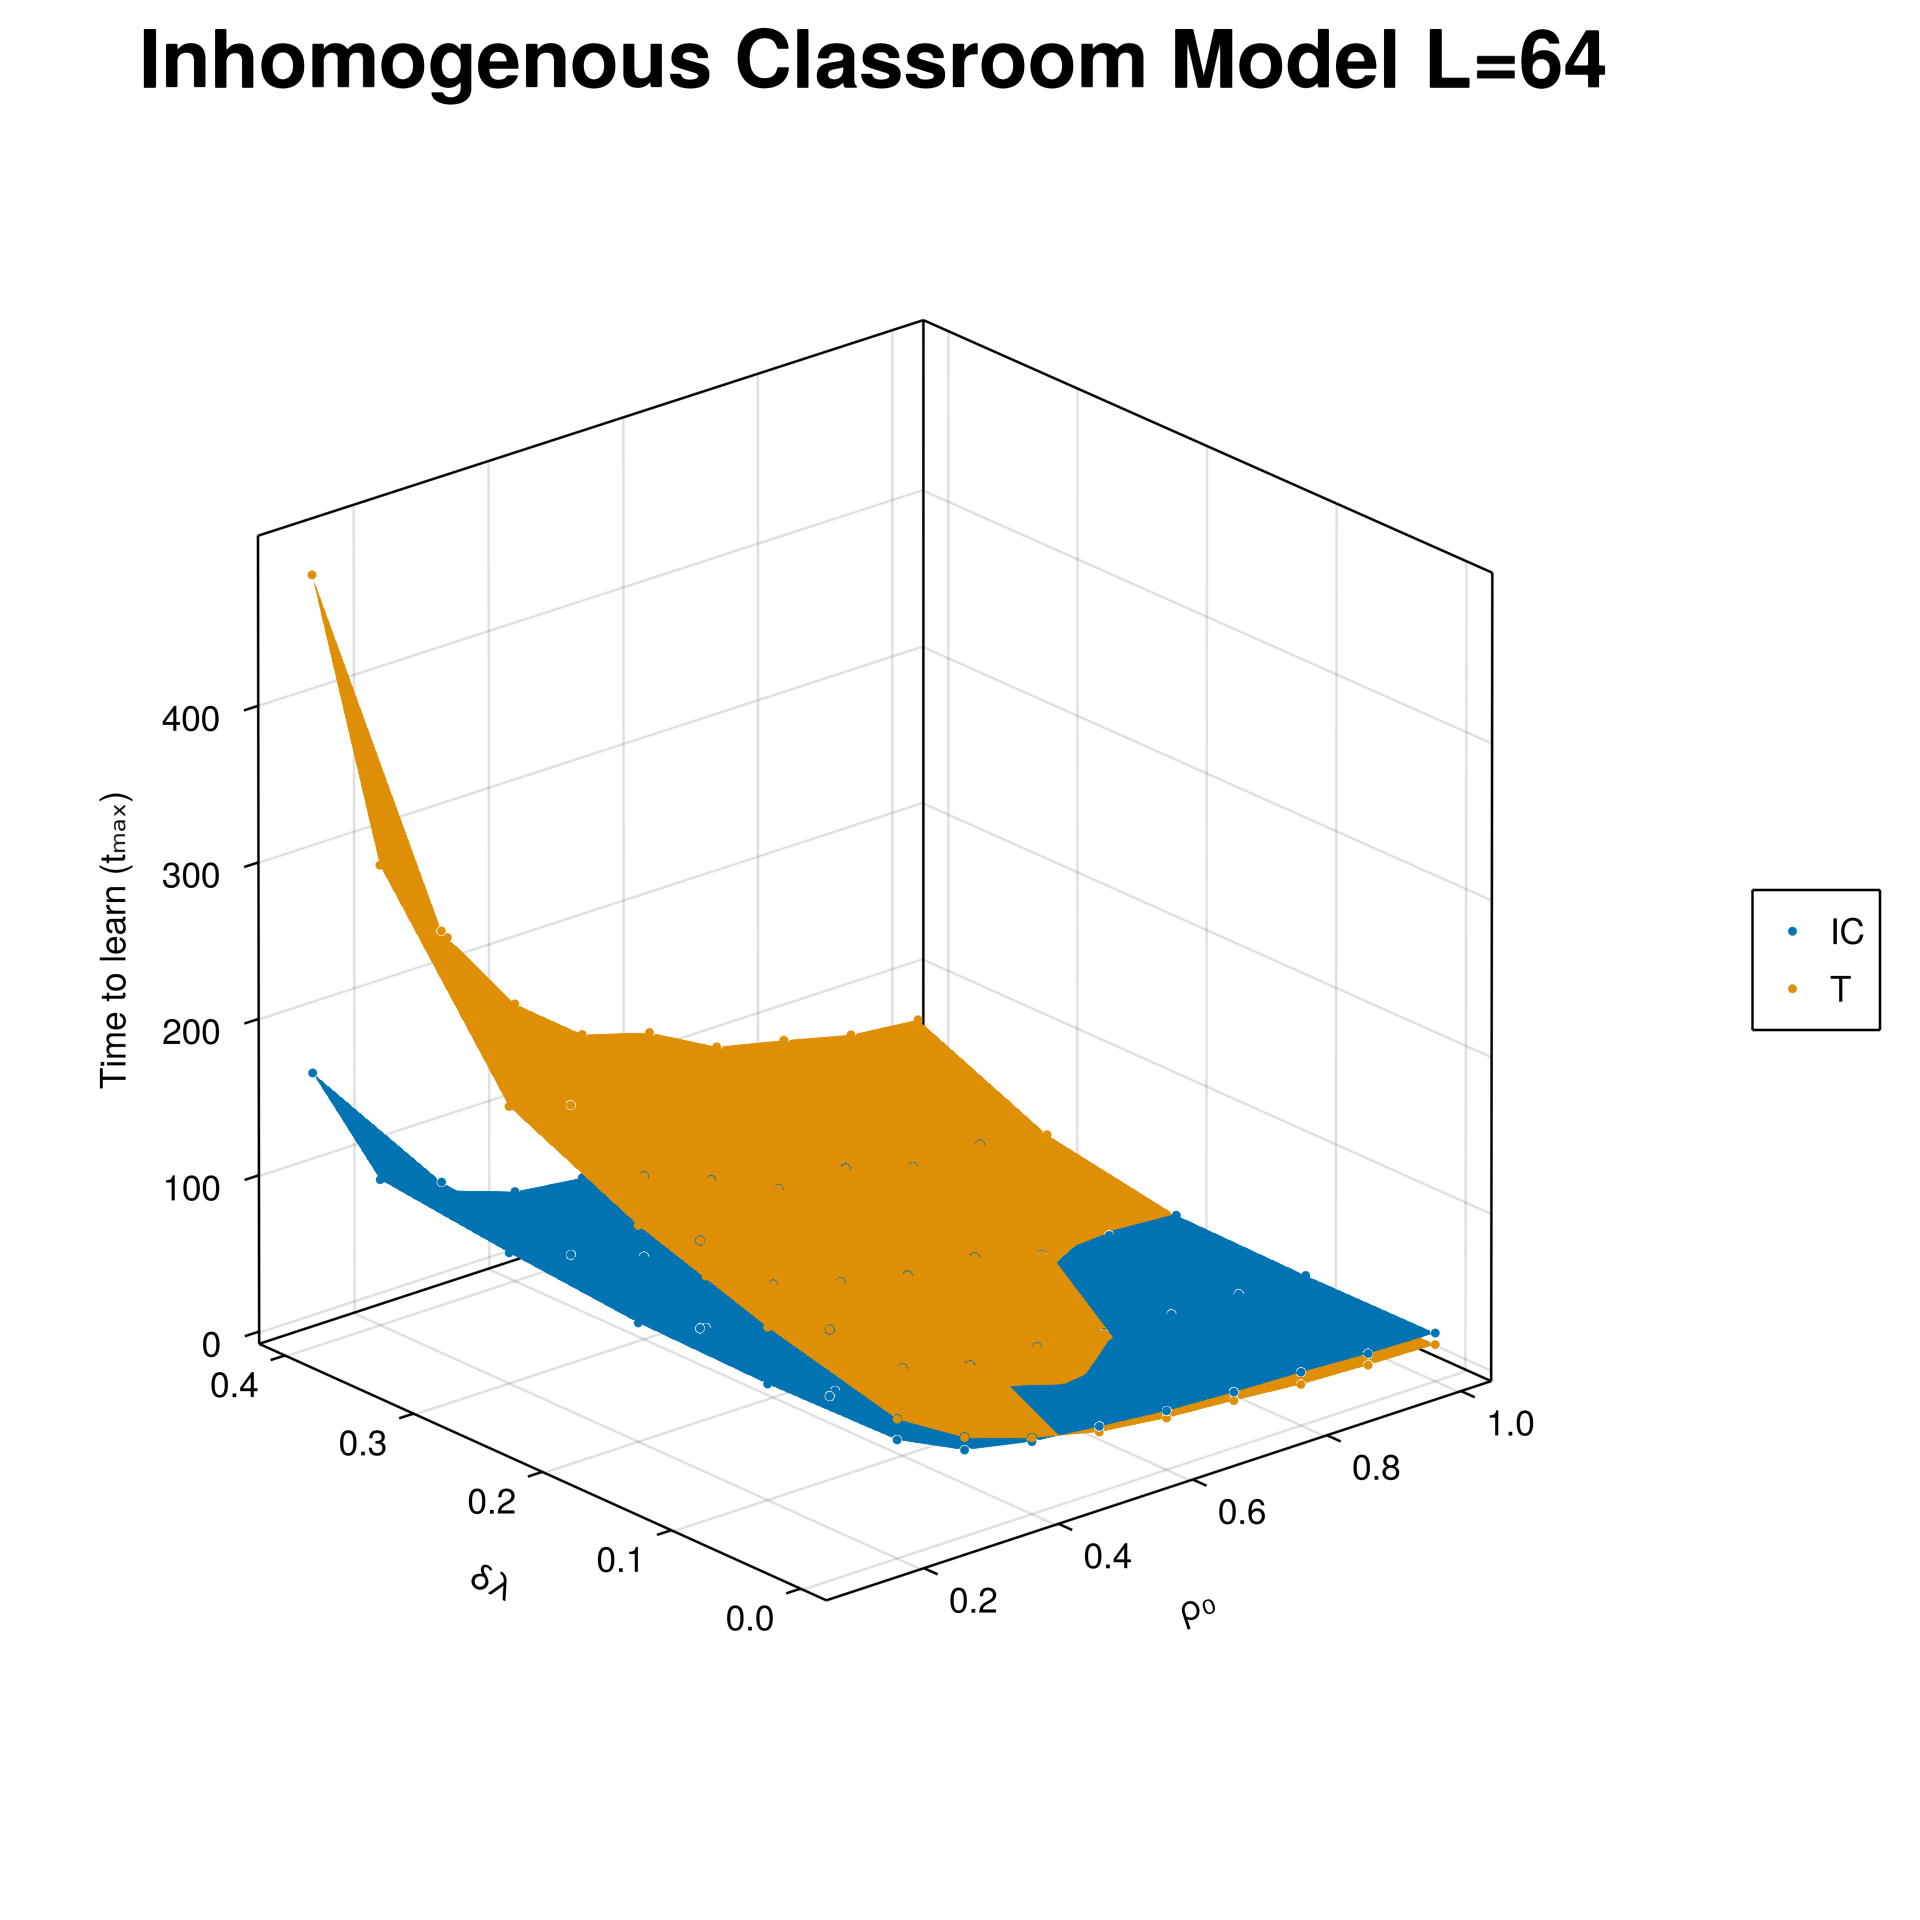
\includegraphics[width=0.40\textwidth]{figures/2D-BPCAIH-analysis/rho-dl-t plots/64.png}}
   \subfigure[$L=96$]{\label{fig:2DBPCAIH rho-dl-t plot 96}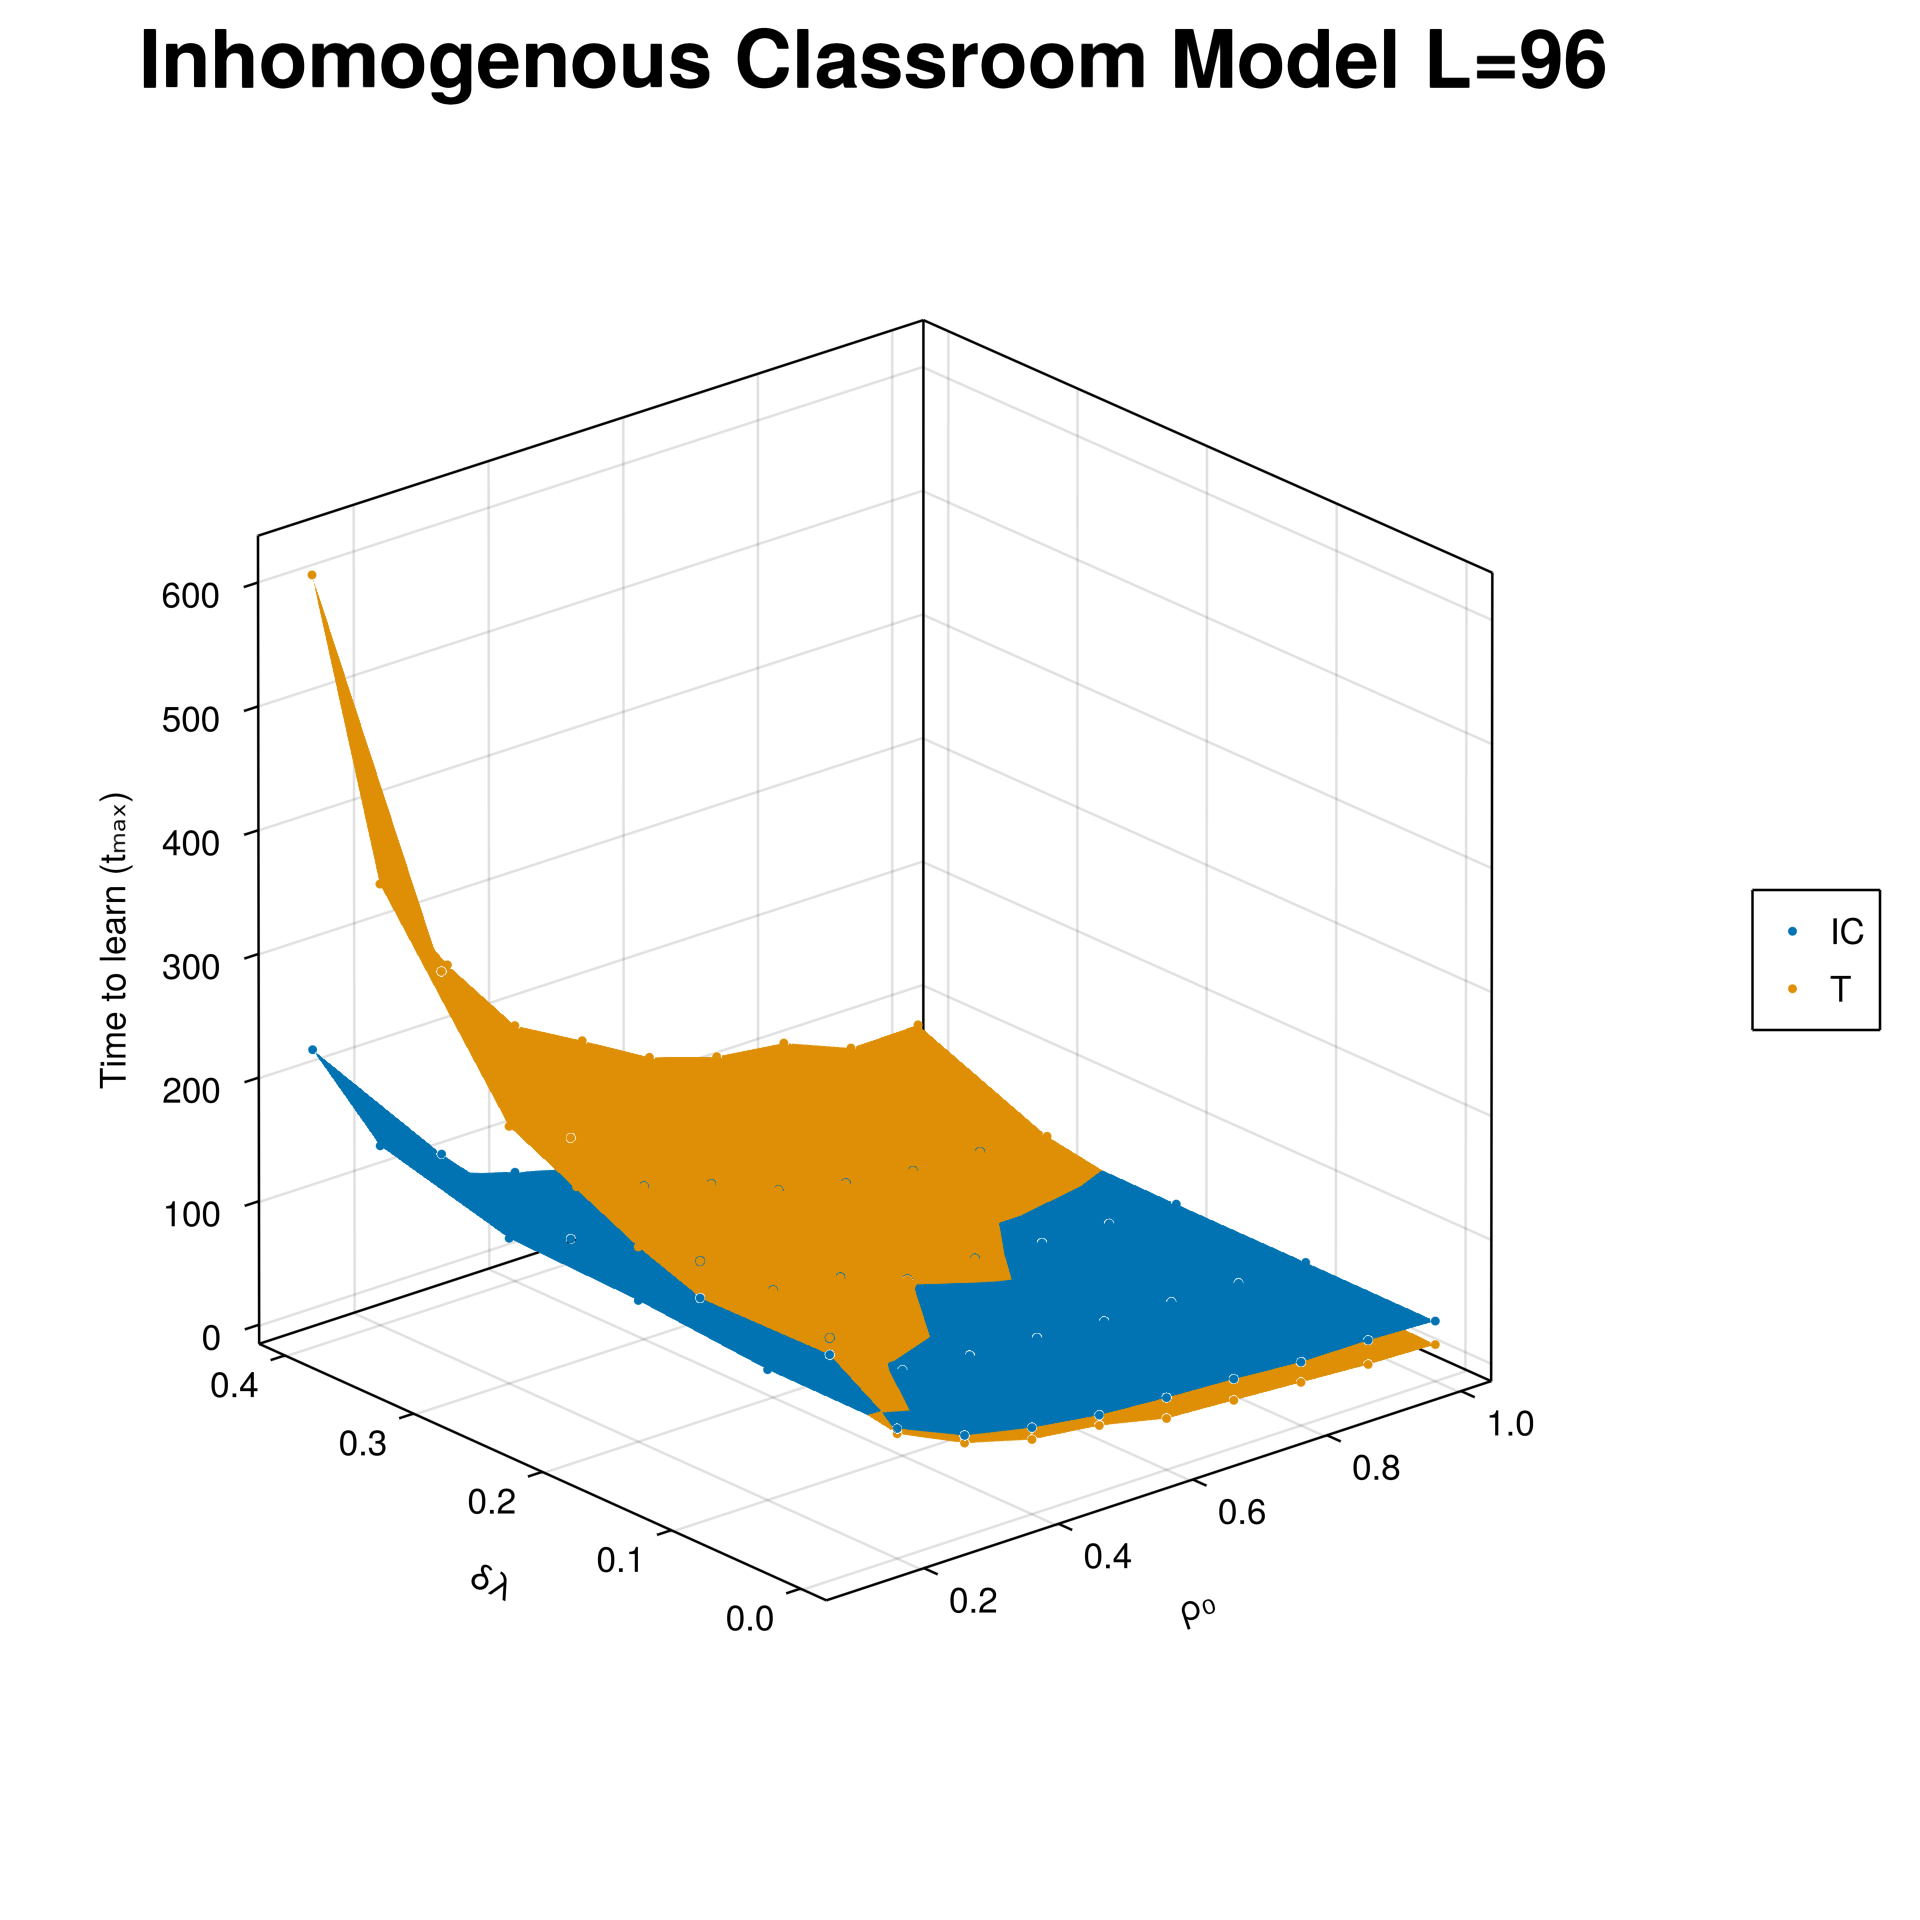
\includegraphics[width=0.40\textwidth]{figures/2D-BPCAIH-analysis/rho-dl-t plots/96.png}}
   \subfigure[$L=128$]{\label{fig:2DBPCAIH rho-dl-t plot 128}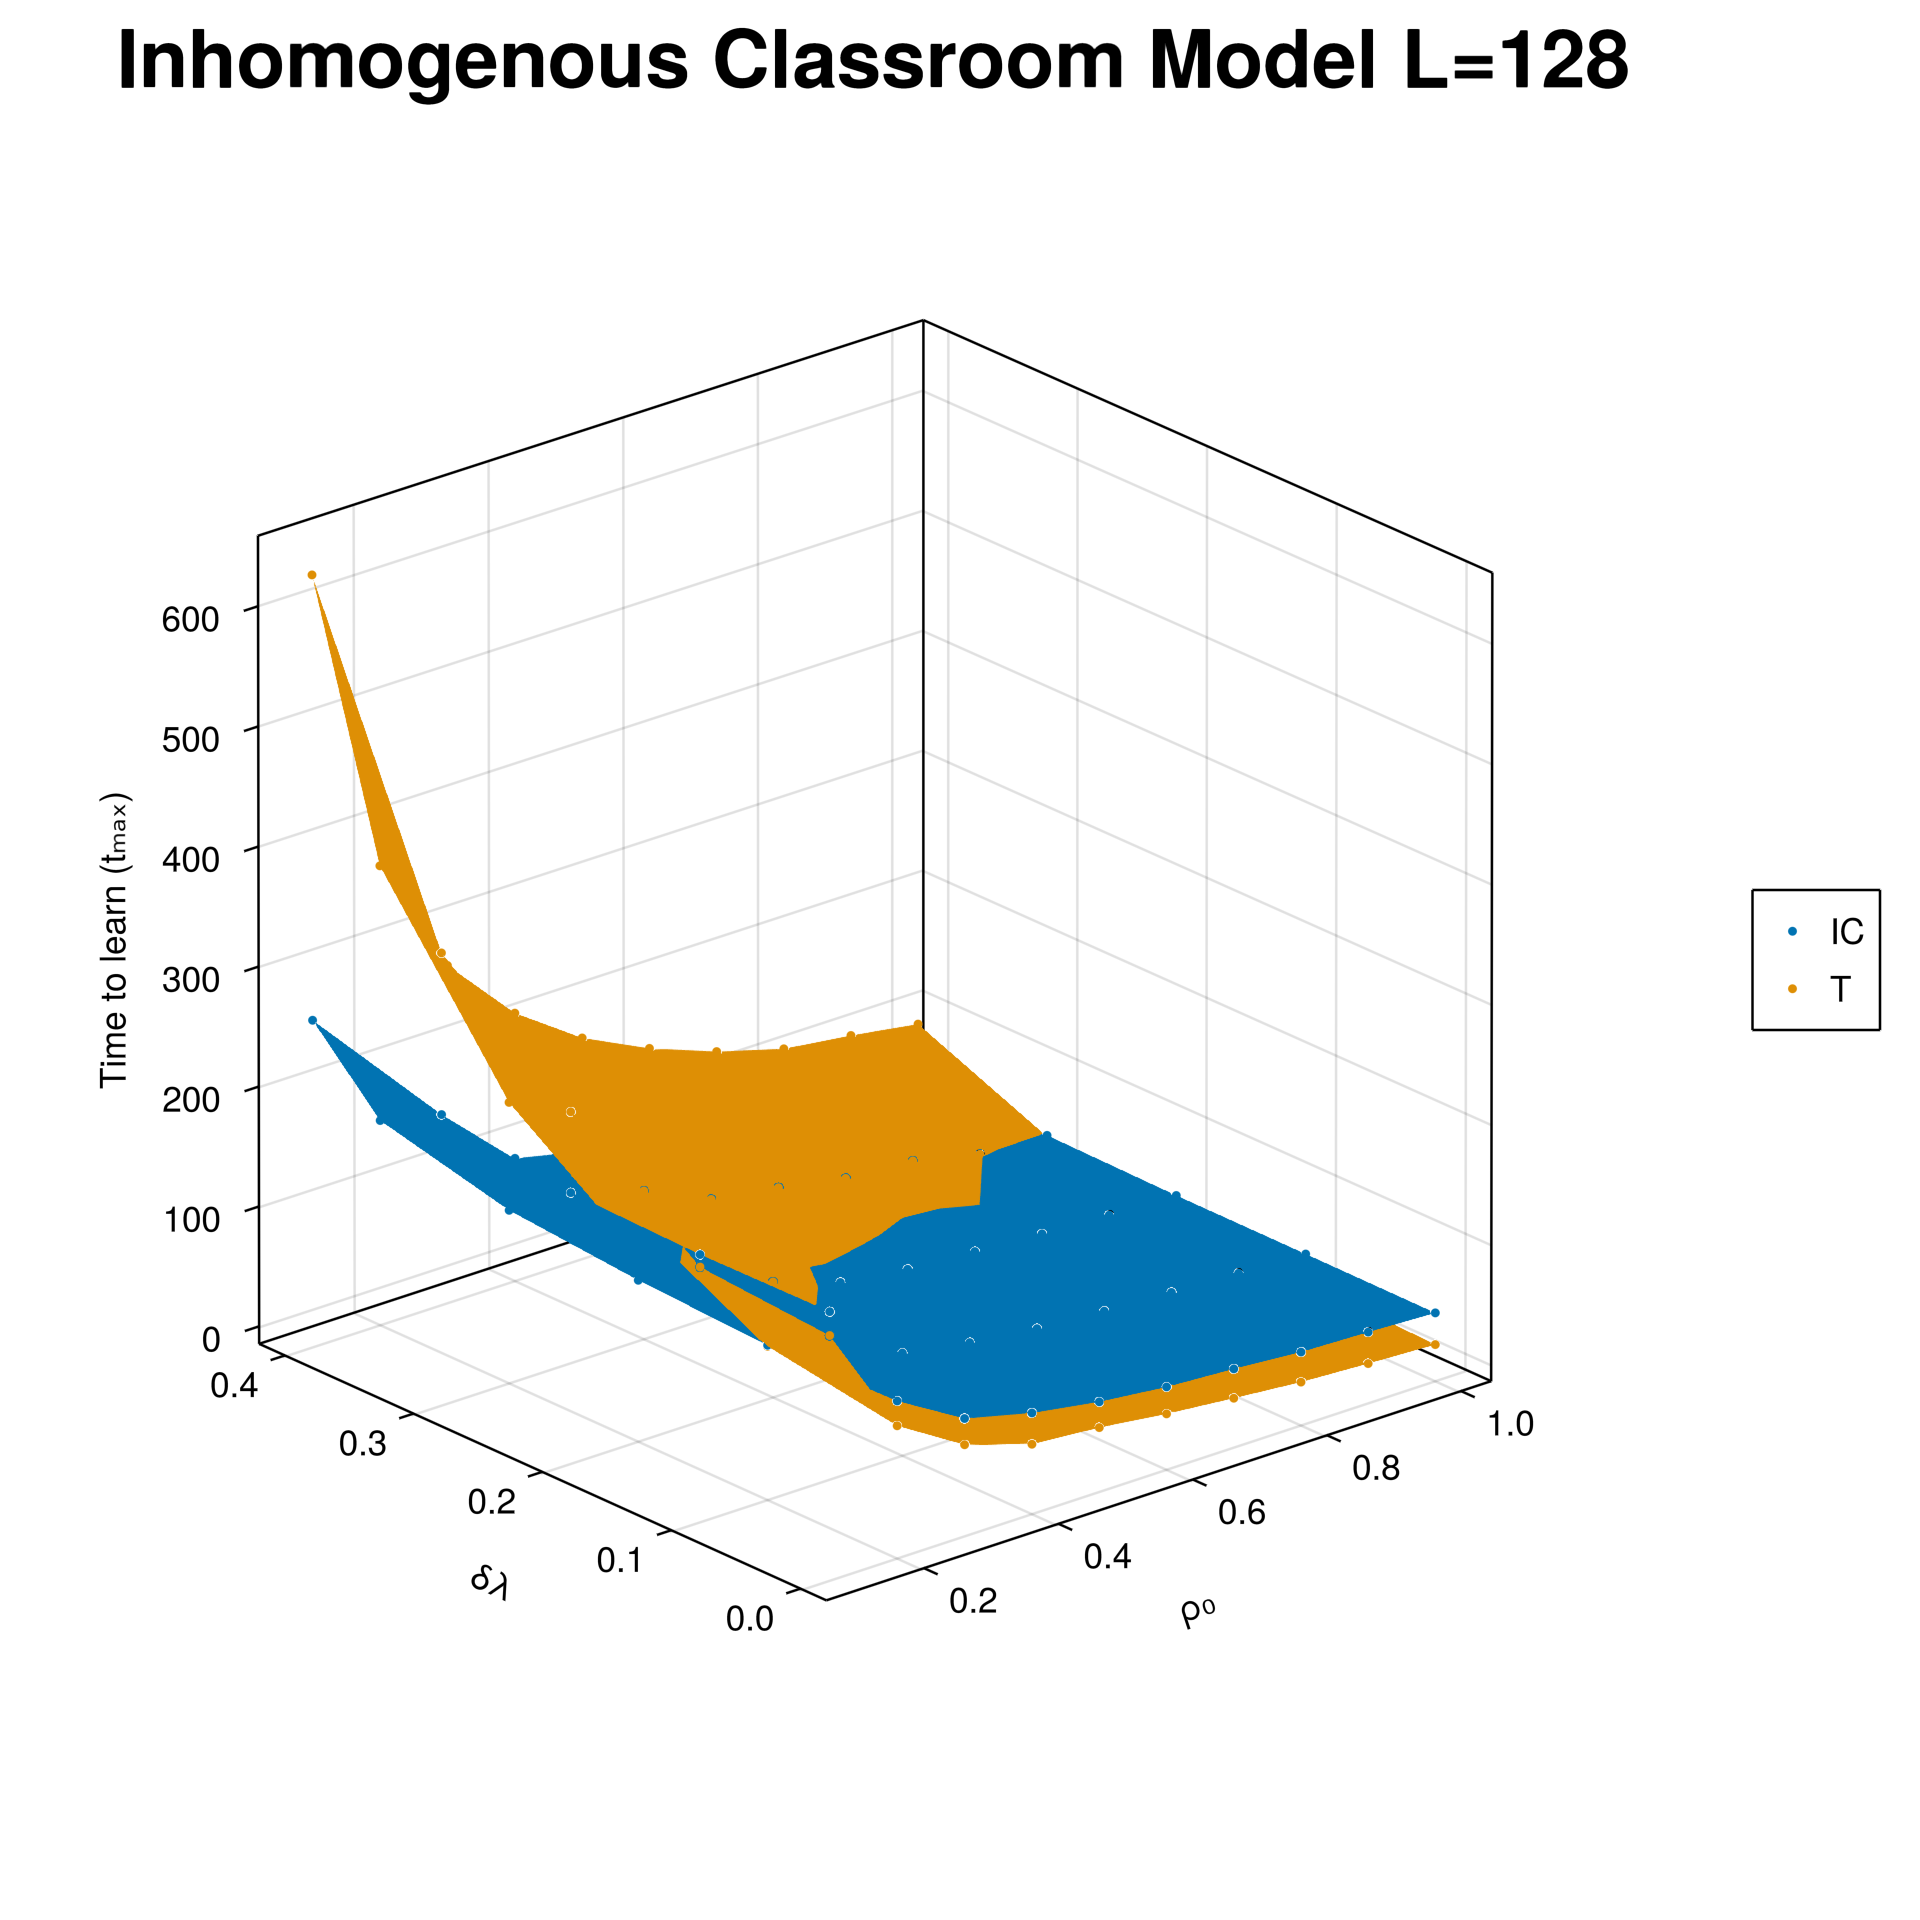
\includegraphics[width=0.40\textwidth]{figures/2D-BPCAIH-analysis/rho-dl-t plots/128.png}}
   \caption[3D plots for the dependence of time to learn $t_{max}$ on both the positional learning factor $\rho_0$ and heterogeneity $\delta\lambda$]{Time to learn $t_{max}$ as a function of positional learning factor $\rho_0$ and heterogeneity $\delta\lambda$ for the heterogeneous models of the PI (inner corner SA) and traditional models with varying positional learning factor. 
   The blue surface represents PI and the orange surface represents traditional instruction.
   Lower time to learn $t_{max}$ indicates better performance.
   }
   \label{fig:2DBPCAIH rho-dl-t plots}
\end{figure}

\newpage % new page after section 3D plots

\section{Conclusions}\label{sec:BPCAIH discussions}
To better model the real world, we introduced heterogeneity to the students' learning rate. 
Adding heterogeneity does not affect the general trend of our instruction models. 
For the case of a heterogeneous system, we still find traditional instruction fares better than PI for larger classes with high positional learning factor $rho_0$.

Besides not affecting the general trend, we found that traditional instuction is more sensitive to heterogeneity. 
As discussed in section \ref{sec:BPCAIH effects on classroom evolution}, the difference in sensitivity is because of the dynamics that were seen in the classes' evolution. 
This is related to the spatio-temporal dynamics of traditional learning models where the fast learning students learn first and the slow learning students learn last.
The time to learn $t_{max}$ for traditional instruction is then dependent on waiting for the slow students.

In contrast to the spatio-temporal dynamics of traditional instruction, the advantage of PI is that it is not as heavily dependent on the students themselves as traditional instruction.
PI is more dependent on the geometry of the classroom and the number of learning sources available to the students.
For the case of PI, the ``wavefront of learning'' (see: section \ref{sec:BPCAIH effects on classroom evolution}) provides students with more than one source of learning, unlike in traditional instruction. 
This phenomenon offsets the increase in the time to learn $t_{max}$ that is caused by waiting for the slow learning students.
PI models therefore have a shorter time to learn $t_{max}$, even though the traditional model initially performs better.

Given the foregoing, initially performing traditional instruction and then proceeding with PI later would maximize each method's strengths. 
The traditional instruction phase would yield high learning rates at the start of the simulation, by allowing the fast learning students to learn first.
The learned students would then be able to help the slow learning students learn in the PI phase, shortening the time to learn $t_{max}$.

As a secondary strategy, if one has to choose to implement only one instruction method, PI is the safe option. Despite not always being the most optimal, the performance advantage of traditional over PI is not as pronounced as the performance advantage of PI over traditional.

% \begin{itemize}
%    \item PI models still better for small classrooms, traditional models better for large class sizes. Same for both homogenous and hetergeneous.
%    \item heterogeneity can sway which set up is advantageous. Low heterogeneity favors traditional models, high heterogeneity favors PI models. Need to add plots for easier explanation.
%    \item Traditional models are more sensitive than heterogeneity. Higher difference, less effective traditional models.
%    \item Initial learning rate for traditional models is fast, but overall time to learn is longer than PI models. Natural consequence: trad then PI. This is what is done currently.
% \end{itemize}
